\documentclass[]{book}
\usepackage{lmodern}
\usepackage{amssymb,amsmath}
\usepackage{ifxetex,ifluatex}
\usepackage{fixltx2e} % provides \textsubscript
\ifnum 0\ifxetex 1\fi\ifluatex 1\fi=0 % if pdftex
  \usepackage[T1]{fontenc}
  \usepackage[utf8]{inputenc}
\else % if luatex or xelatex
  \ifxetex
    \usepackage{mathspec}
  \else
    \usepackage{fontspec}
  \fi
  \defaultfontfeatures{Ligatures=TeX,Scale=MatchLowercase}
\fi
% use upquote if available, for straight quotes in verbatim environments
\IfFileExists{upquote.sty}{\usepackage{upquote}}{}
% use microtype if available
\IfFileExists{microtype.sty}{%
\usepackage{microtype}
\UseMicrotypeSet[protrusion]{basicmath} % disable protrusion for tt fonts
}{}
\usepackage[margin=1in]{geometry}
\usepackage{hyperref}
\hypersetup{unicode=true,
            pdftitle={Introducción al software estadístico R},
            pdfauthor={Dae-Jin Lee \textless{} dlee@bcamath.org \textgreater{}},
            pdfborder={0 0 0},
            breaklinks=true}
\urlstyle{same}  % don't use monospace font for urls
\usepackage{natbib}
\bibliographystyle{apalike}
\usepackage{color}
\usepackage{fancyvrb}
\newcommand{\VerbBar}{|}
\newcommand{\VERB}{\Verb[commandchars=\\\{\}]}
\DefineVerbatimEnvironment{Highlighting}{Verbatim}{commandchars=\\\{\}}
% Add ',fontsize=\small' for more characters per line
\usepackage{framed}
\definecolor{shadecolor}{RGB}{248,248,248}
\newenvironment{Shaded}{\begin{snugshade}}{\end{snugshade}}
\newcommand{\KeywordTok}[1]{\textcolor[rgb]{0.13,0.29,0.53}{\textbf{#1}}}
\newcommand{\DataTypeTok}[1]{\textcolor[rgb]{0.13,0.29,0.53}{#1}}
\newcommand{\DecValTok}[1]{\textcolor[rgb]{0.00,0.00,0.81}{#1}}
\newcommand{\BaseNTok}[1]{\textcolor[rgb]{0.00,0.00,0.81}{#1}}
\newcommand{\FloatTok}[1]{\textcolor[rgb]{0.00,0.00,0.81}{#1}}
\newcommand{\ConstantTok}[1]{\textcolor[rgb]{0.00,0.00,0.00}{#1}}
\newcommand{\CharTok}[1]{\textcolor[rgb]{0.31,0.60,0.02}{#1}}
\newcommand{\SpecialCharTok}[1]{\textcolor[rgb]{0.00,0.00,0.00}{#1}}
\newcommand{\StringTok}[1]{\textcolor[rgb]{0.31,0.60,0.02}{#1}}
\newcommand{\VerbatimStringTok}[1]{\textcolor[rgb]{0.31,0.60,0.02}{#1}}
\newcommand{\SpecialStringTok}[1]{\textcolor[rgb]{0.31,0.60,0.02}{#1}}
\newcommand{\ImportTok}[1]{#1}
\newcommand{\CommentTok}[1]{\textcolor[rgb]{0.56,0.35,0.01}{\textit{#1}}}
\newcommand{\DocumentationTok}[1]{\textcolor[rgb]{0.56,0.35,0.01}{\textbf{\textit{#1}}}}
\newcommand{\AnnotationTok}[1]{\textcolor[rgb]{0.56,0.35,0.01}{\textbf{\textit{#1}}}}
\newcommand{\CommentVarTok}[1]{\textcolor[rgb]{0.56,0.35,0.01}{\textbf{\textit{#1}}}}
\newcommand{\OtherTok}[1]{\textcolor[rgb]{0.56,0.35,0.01}{#1}}
\newcommand{\FunctionTok}[1]{\textcolor[rgb]{0.00,0.00,0.00}{#1}}
\newcommand{\VariableTok}[1]{\textcolor[rgb]{0.00,0.00,0.00}{#1}}
\newcommand{\ControlFlowTok}[1]{\textcolor[rgb]{0.13,0.29,0.53}{\textbf{#1}}}
\newcommand{\OperatorTok}[1]{\textcolor[rgb]{0.81,0.36,0.00}{\textbf{#1}}}
\newcommand{\BuiltInTok}[1]{#1}
\newcommand{\ExtensionTok}[1]{#1}
\newcommand{\PreprocessorTok}[1]{\textcolor[rgb]{0.56,0.35,0.01}{\textit{#1}}}
\newcommand{\AttributeTok}[1]{\textcolor[rgb]{0.77,0.63,0.00}{#1}}
\newcommand{\RegionMarkerTok}[1]{#1}
\newcommand{\InformationTok}[1]{\textcolor[rgb]{0.56,0.35,0.01}{\textbf{\textit{#1}}}}
\newcommand{\WarningTok}[1]{\textcolor[rgb]{0.56,0.35,0.01}{\textbf{\textit{#1}}}}
\newcommand{\AlertTok}[1]{\textcolor[rgb]{0.94,0.16,0.16}{#1}}
\newcommand{\ErrorTok}[1]{\textcolor[rgb]{0.64,0.00,0.00}{\textbf{#1}}}
\newcommand{\NormalTok}[1]{#1}
\usepackage{longtable,booktabs}
\usepackage{graphicx,grffile}
\makeatletter
\def\maxwidth{\ifdim\Gin@nat@width>\linewidth\linewidth\else\Gin@nat@width\fi}
\def\maxheight{\ifdim\Gin@nat@height>\textheight\textheight\else\Gin@nat@height\fi}
\makeatother
% Scale images if necessary, so that they will not overflow the page
% margins by default, and it is still possible to overwrite the defaults
% using explicit options in \includegraphics[width, height, ...]{}
\setkeys{Gin}{width=\maxwidth,height=\maxheight,keepaspectratio}
\IfFileExists{parskip.sty}{%
\usepackage{parskip}
}{% else
\setlength{\parindent}{0pt}
\setlength{\parskip}{6pt plus 2pt minus 1pt}
}
\setlength{\emergencystretch}{3em}  % prevent overfull lines
\providecommand{\tightlist}{%
  \setlength{\itemsep}{0pt}\setlength{\parskip}{0pt}}
\setcounter{secnumdepth}{5}
% Redefines (sub)paragraphs to behave more like sections
\ifx\paragraph\undefined\else
\let\oldparagraph\paragraph
\renewcommand{\paragraph}[1]{\oldparagraph{#1}\mbox{}}
\fi
\ifx\subparagraph\undefined\else
\let\oldsubparagraph\subparagraph
\renewcommand{\subparagraph}[1]{\oldsubparagraph{#1}\mbox{}}
\fi

%%% Use protect on footnotes to avoid problems with footnotes in titles
\let\rmarkdownfootnote\footnote%
\def\footnote{\protect\rmarkdownfootnote}

%%% Change title format to be more compact
\usepackage{titling}

% Create subtitle command for use in maketitle
\newcommand{\subtitle}[1]{
  \posttitle{
    \begin{center}\large#1\end{center}
    }
}

\setlength{\droptitle}{-2em}

  \title{Introducción al software estadístico \texttt{R}}
    \pretitle{\vspace{\droptitle}\centering\huge}
  \posttitle{\par}
    \author{Dae-Jin Lee \textless{}
\href{mailto:dlee@bcamath.org}{\nolinkurl{dlee@bcamath.org}}
\textgreater{}}
    \preauthor{\centering\large\emph}
  \postauthor{\par}
      \predate{\centering\large\emph}
  \postdate{\par}
    \date{Marzo 2019}

\usepackage{booktabs}
\usepackage[spanish]{babel}
\usepackage{amsthm}
\makeatletter
\def\thm@space@setup{%
  \thm@preskip=8pt plus 2pt minus 4pt
  \thm@postskip=\thm@preskip
}
\makeatother

\begin{document}
\maketitle

{
\setcounter{tocdepth}{1}
\tableofcontents
}
\chapter{Información y
pre-requisitos}\label{informacion-y-pre-requisitos}

\begin{itemize}
\item
  \textbf{Requisitos:}

  \begin{itemize}
  \tightlist
  \item
    Última versión del software \texttt{R} (https://www.r-project.org)
  \item
    \texttt{Rstudio} (https://www.rstudio.com).
  \end{itemize}
\end{itemize}

~

\begin{itemize}
\item
  \textbf{Horario:}

  \begin{itemize}
  \tightlist
  \item
    Día 11 de marzo 10:30 a 14:30 horas
  \item
    Días 12 y 13 de marzo de 09.00 a 13.00 horas
  \item
    Día 14 de marzo 09.00 a 12.00 horas
  \end{itemize}
\end{itemize}

~

\begin{itemize}
\tightlist
\item
  \textbf{Objetivos del curso}
\end{itemize}

El curso proporcionará conocimientos básicos y habilidades para utilizar
el software estadístico \texttt{R} como entorno de trabajo y análisis de
datos. Para ello, el curso ofrecerá una visión general de las
herramientas ofrecidas por \texttt{R}, por ejemplo, desde el manejo de
matrices y conjuntos de datos, a representaciones gráficas, pruebas y
análisis estadísticos, programación en \texttt{R} y técnicas de
modelización estadística y aprendizaje automático.

El objetivo es que al final del curso todos se hayan familiarizado con
el software estadístico \texttt{R}.

\begin{itemize}
\item
  \textbf{Material complementario (en inglés)}

  \begin{itemize}
  \item
    \href{https://www.calvin.edu/~scofield/courses/m143/materials/RcmdsFromClass.pdf}{Table
    of useful \texttt{R} commands}
  \item
    \href{https://www.rstudio.com/wp-content/uploads/2016/10/r-cheat-sheet-3.pdf}{Base
    \texttt{R} cheatsheet}
  \item
    \href{http://www.webpages.uidaho.edu/~stevel/251/comR.pdf}{Not so
    short list of \texttt{R} commands}
  \item
    \href{http://r4ds.had.co.nz/}{Additional material: \texttt{R} for
    Data Science} or \href{http://courses.had.co.nz/}{here}
  \item
    Some interesting links:

    \begin{itemize}
    \item
      \href{http://kbroman.org/pages/talks.html}{Karl Broman's talks}
    \item
      \href{http://genomicsclass.github.io/book/pages/plots_to_avoid.html}{Plots
      to avoid}
    \item
      \href{http://rseek.org/}{RSeek} - a Google search engine for R
      documentation and help. A MUST see!
    \end{itemize}
  \end{itemize}
\end{itemize}

\chapter{\texorpdfstring{Introducción al software estadístico
\texttt{R}}{Introducción al software estadístico R}}\label{intro}

\texttt{R} es un entorno y lenguaje de programación orientado al
análisis estadístico, al cálculo, manipulación de datos, y
representaciones gráficas. Es multiplataforma y parte del sistema GNU y
se distribuye con licencia GNU-GPL.

Más información
\href{https://es.wikipedia.org/wiki/R_(lenguaje_de_programaci\%C3\%B3n)}{aquí}.
~

\section{\texorpdfstring{Algunas cuestiones a tener en cuenta sobre
\texttt{R}}{Algunas cuestiones a tener en cuenta sobre R}}\label{algunas-cuestiones-a-tener-en-cuenta-sobre-r}

\begin{itemize}
\item
  \texttt{R} distingue mayúsculas y minúsculas.
\item
  Para asignar contenido a un objeto usamos \texttt{\textless{}-}. Por
  ejemplo, \texttt{x\ \textless{}-\ 10} asigna a \texttt{x} el valor
  \texttt{10}. También podemos usar =.
\item
  Para ver el contenido de un objeto simplemente escribimos su nombre.
\item
  Para usar los comandos escribimos el nombre del comando seguido de sus
  argumentos entre paréntesis. Por ejemplo, \texttt{ls()}da una lista de
  los objetos en el área de trabajo. Como no usamos argumentos
  (diferentes a los que el comando tenga por defecto) no escribimos nada
  en el paréntesis.
\item
  Para obtener ayuda usamos el comando \texttt{help}. Por ejemplo,
  \texttt{help(mean)} para obtener ayuda sobre el comando \texttt{mean}
  que calcula la media.
\end{itemize}

\section{Guardar los resultados y el
código}\label{guardar-los-resultados-y-el-codigo}

\begin{itemize}
\item
  Al entrar en \texttt{R}, se considera cierto directorio por defecto
  como el directorio de trabajo. Este directorio puede cambiarse en el
  menú Archivo, \texttt{Cambiar\ dir}\ldots{} Resulta conveniente tener
  un directorio diferente para cada proyecto que realicemos.
\item
  Al salir de \texttt{R} se nos pregunta
  \texttt{Guardar\ imagen\ de\ área\ de\ trabajo?}. Si respondemos
  afirmativamente, se crea un fichero \texttt{.RData} en el directorio
  de trabajo que contiene todos los objetos del área de trabajo en el
  momento de salir. Posteriormente, haciendo doble clic en este fichero
  podremos entrar en \texttt{R} y seguir trabajando exactamente en el
  mismo punto en que lo habíamos dejado al salir.
\item
  Alternativamente podemos usar los comandos \texttt{save} y
  \texttt{load} para guardar y recuperar objetos. Consulta la ayuda de
  estos comandos para ver sus diferentes opciones.
\item
  Todos los comandos y código de \texttt{R} se pueden guardar en un
  fichero de texto (con \texttt{extensión.R}) dentro del directorio de
  trabajo. El comando source se puede usar para ejecutar todo el código
  contenido en un fichero de texto. En el menú \texttt{Archivo},
  \texttt{Abrir\ script} podemos acceder a un editor muy simple en el
  que poder ir escribiendo el código.
\end{itemize}

\section{Rstudio}\label{rstudio}

RStudio es un IDE (Integrated Development Environment, o Entorno de
Desarrollo Integrado) de código abierto para \texttt{R}, que permite
interactuar con \texttt{R} de manera muy simple.

Entre otras ventajas, Rstudio utiliza diferentes colores para las
distintas clases de objetos de \texttt{R}, permite autocompletar código,
incluye un sistema de menús de ayuda muy completo, cuenta con un potente
sistema para la gestión, descarga y construcción de librerías, dispone
de un depurador de código que detecta posibles errores de sintaxis, es
multiplataforma (existen versiones para Windows, Linux y Mac).

\begin{figure}

{\centering 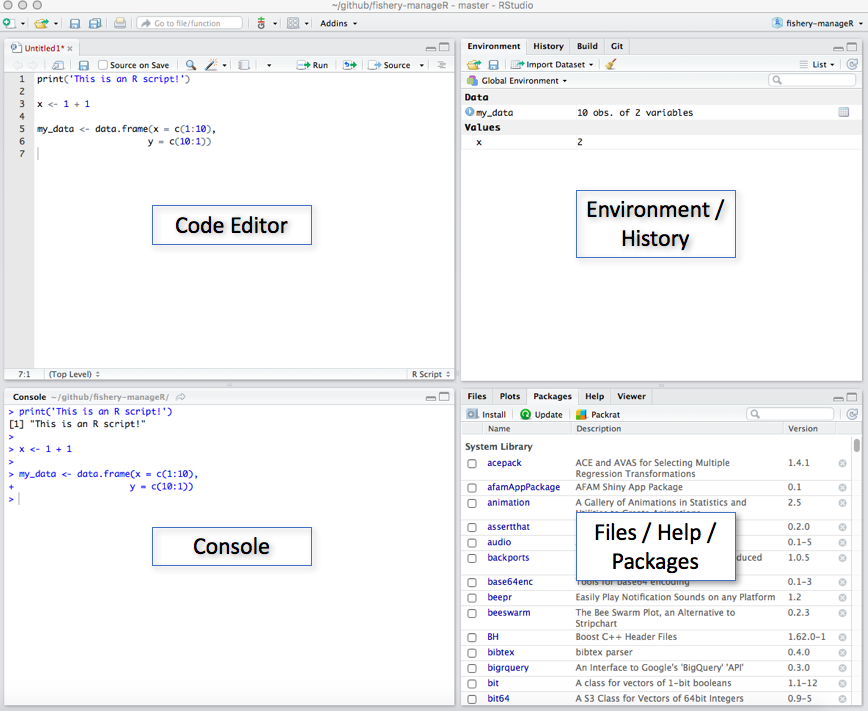
\includegraphics[width=1\linewidth]{figures/rstudio_ide} 

}

\caption{Interfaz RStudio}\label{fig:pressure}
\end{figure}

A la izquierda, la consola donde se ejecutan los comandos de \texttt{R}.

A la derecha, en la parte superior, tenemos una ventana que muestra
nuestro entorno (environment) de trabajo, en el que iremos viendo las
variables y funciones que vayamos cargando, creando, etc. Obsérvese que
esta ventana tiene algunos iconos que permiten guardar el contenido de
la memoria, cargar el contenido de la memoria de una sesión de trabajo
anterior, importar archivos de datos que se hayan guardado como texto, y
limpiar el contenido de la memoria.

A la derecha, en la parte inferior, se muestra el contenido de nuestro
directorio home donde R arranca por defecto. Observemos que esta ventana
tiene varias pestañas:

\begin{itemize}
\tightlist
\item
  \textbf{Files:} archivos en el directorio actual.
\item
  \textbf{Plots:} en esta ventana se irán mostrando los gráficos que
  generemos con el programa.
\item
  \textbf{Packages:} permite ver qué librerías (colecciones de funciones
  que extienen la funcionalidad de R) tenemos instaladas; asimismo nos
  permite descargar e instalar nuevas librerías.
\item
  \textbf{Help:} permite acceder a ayuda sobre R.
\item
  \textbf{Viewer:} Permite acceder a contenido web local.
\end{itemize}

\section{\texorpdfstring{Instalar un paquete de
\texttt{R}}{Instalar un paquete de R}}\label{instalar-un-paquete-de-r}

\begin{itemize}
\tightlist
\item
  Desde la consola
\end{itemize}

\begin{Shaded}
\begin{Highlighting}[]
\KeywordTok{install.packages}\NormalTok{(}\StringTok{"< Nombre del paquete >"}\NormalTok{)}
\end{Highlighting}
\end{Shaded}

\begin{itemize}
\tightlist
\item
  Ejemplo:
\end{itemize}

\begin{Shaded}
\begin{Highlighting}[]
\KeywordTok{install.packages}\NormalTok{(}\StringTok{"DAAG"}\NormalTok{)}
\CommentTok{# Varios paquetes con el comando c("< Paquete 1 >","< Paquete 2 >")}
\KeywordTok{install.packages}\NormalTok{(}\KeywordTok{c}\NormalTok{(}\StringTok{"DAAG"}\NormalTok{,}\StringTok{"psych"}\NormalTok{,}\StringTok{"gdata"}\NormalTok{,}\StringTok{"foreign"}\NormalTok{,}\StringTok{"Hmisc"}\NormalTok{,}\StringTok{"xlsx"}\NormalTok{,}
                   \StringTok{"MASS"}\NormalTok{,}\StringTok{"calibrate"}\NormalTok{,}\StringTok{"corrplot"}\NormalTok{,}\StringTok{"fields"}\NormalTok{,}\StringTok{"RColorBrewer"}\NormalTok{,}
                   \StringTok{"ggplot2"}\NormalTok{,}\StringTok{"lattice"}\NormalTok{,}\StringTok{"visreg"}\NormalTok{,}
                   \StringTok{"car"}\NormalTok{,}\StringTok{"InformationValue"}\NormalTok{,}\StringTok{"ROCR"}\NormalTok{)) }
\end{Highlighting}
\end{Shaded}

\begin{itemize}
\tightlist
\item
  Desde Rstudio: \texttt{Packages\ \textgreater{}\ Install}
\end{itemize}

\section{\texorpdfstring{Empezando con
\texttt{R}}{Empezando con R}}\label{empezando-con-r}

\begin{itemize}
\tightlist
\item
  Obtener el directorio de trabajo o \emph{working directory}
\end{itemize}

\begin{Shaded}
\begin{Highlighting}[]
\KeywordTok{getwd}\NormalTok{() }
\end{Highlighting}
\end{Shaded}

\begin{itemize}
\tightlist
\item
  listar los objetos en el espacio de trabajo o \emph{workspace}
\end{itemize}

\begin{Shaded}
\begin{Highlighting}[]
\KeywordTok{ls}\NormalTok{()}
\end{Highlighting}
\end{Shaded}

\begin{itemize}
\tightlist
\item
  Definir el \emph{working directory}
\end{itemize}

\begin{Shaded}
\begin{Highlighting}[]
\KeywordTok{setwd}\NormalTok{(}\StringTok{"/Users/dlee"}\NormalTok{) }
\end{Highlighting}
\end{Shaded}

\begin{itemize}
\item
  Desde Rstudio:
  \texttt{Files\ \textgreater{}\ Click\ en\ ...\ \textgreater{}\ More\ \textgreater{}\ Set\ as\ workind\ directory}
\item
  Ver los últimos comandos utilizados en la consola
\end{itemize}

\begin{Shaded}
\begin{Highlighting}[]
\KeywordTok{history}\NormalTok{() }\CommentTok{# mostrar los últimos 25 comandos}
\KeywordTok{history}\NormalTok{(}\DataTypeTok{max.show=}\OtherTok{Inf}\NormalTok{) }\CommentTok{# mostrar todos los comandos anteriores}
\end{Highlighting}
\end{Shaded}

\begin{itemize}
\tightlist
\item
  Guardar el historial de comandos
\end{itemize}

\begin{Shaded}
\begin{Highlighting}[]
\KeywordTok{savehistory}\NormalTok{(}\DataTypeTok{file=}\StringTok{"myfile"}\NormalTok{) }\CommentTok{# el valor por defecto es ".Rhistory"}
\end{Highlighting}
\end{Shaded}

\begin{itemize}
\tightlist
\item
  Cargar los commandos guardados en una sesión anterior
\end{itemize}

\begin{Shaded}
\begin{Highlighting}[]
\KeywordTok{loadhistory}\NormalTok{(}\DataTypeTok{file=}\StringTok{"myfile"}\NormalTok{) }\CommentTok{# el valor por defecto es ".Rhistory"}
\end{Highlighting}
\end{Shaded}

\begin{itemize}
\tightlist
\item
  Salvar todo el \textbf{workspace} en un fichero \texttt{.RData}
\end{itemize}

\begin{Shaded}
\begin{Highlighting}[]
\KeywordTok{save.image}\NormalTok{()}
\end{Highlighting}
\end{Shaded}

\begin{itemize}
\tightlist
\item
  Guardar objectos especificos a un fichero (si no se especifica la ruta
  en el ordenador, se guardará en el directorio actual de trabajo).
\end{itemize}

\begin{Shaded}
\begin{Highlighting}[]
\KeywordTok{save}\NormalTok{(}\OperatorTok{<}\NormalTok{object list}\OperatorTok{>}\NormalTok{,}\DataTypeTok{file=}\StringTok{"myfile.RData"}\NormalTok{) }
\end{Highlighting}
\end{Shaded}

\begin{itemize}
\tightlist
\item
  Cargar un \emph{workspace} en la sesión
\end{itemize}

\begin{Shaded}
\begin{Highlighting}[]
\KeywordTok{load}\NormalTok{(}\StringTok{"myfile.RData"}\NormalTok{) }
\end{Highlighting}
\end{Shaded}

\begin{itemize}
\tightlist
\item
  Salir de \texttt{R}. Por defecto \texttt{R} pregunta si deseas guardar
  la sesión.
\end{itemize}

\begin{Shaded}
\begin{Highlighting}[]
\KeywordTok{q}\NormalTok{()}
\end{Highlighting}
\end{Shaded}

\section{\texorpdfstring{Instalar y cargar librerías en
\texttt{R}}{Instalar y cargar librerías en R}}\label{instalar-y-cargar-librerias-en-r}

\begin{Shaded}
\begin{Highlighting}[]
\KeywordTok{install.packages}\NormalTok{(}\StringTok{"DAAG"}\NormalTok{) }\CommentTok{# (Data Analysis And Graphics)}
\end{Highlighting}
\end{Shaded}

\begin{itemize}
\tightlist
\item
  Una vez instalada la librería, tenemos que cargarla con el comando
  \texttt{library} o \texttt{require}
\end{itemize}

\begin{Shaded}
\begin{Highlighting}[]
\KeywordTok{library}\NormalTok{(DAAG) }\CommentTok{# o require(DAAG)}
\end{Highlighting}
\end{Shaded}

\section{Lectura de datos}\label{lectura-de-datos}

Consola de \texttt{R}

\begin{Shaded}
\begin{Highlighting}[]
\NormalTok{x <-}\StringTok{ }\KeywordTok{c}\NormalTok{(}\FloatTok{7.82}\NormalTok{,}\FloatTok{8.00}\NormalTok{,}\FloatTok{7.95}\NormalTok{) }\CommentTok{# c de "combinar"}
\NormalTok{x}
\end{Highlighting}
\end{Shaded}

\begin{verbatim}
## [1] 7.82 8.00 7.95
\end{verbatim}

Otra forma es mediante la función \texttt{scan()}

\begin{Shaded}
\begin{Highlighting}[]
\NormalTok{x <-}\StringTok{ }\KeywordTok{scan}\NormalTok{()  }\CommentTok{# introducir números seguidos de ENTER y terminar con un ENTER}
\DecValTok{1}\OperatorTok{:}\StringTok{ }\FloatTok{7.82}
\DecValTok{2}\OperatorTok{:}\StringTok{ }\FloatTok{8.00}
\DecValTok{3}\OperatorTok{:}\StringTok{ }\FloatTok{7.95}
\DecValTok{4}\OperatorTok{:}\StringTok{ }
\NormalTok{Read }\DecValTok{3}\NormalTok{ items}
\end{Highlighting}
\end{Shaded}

Para crear un vector de caracteres \texttt{""}

\begin{Shaded}
\begin{Highlighting}[]
\NormalTok{id <-}\StringTok{ }\KeywordTok{c}\NormalTok{(}\StringTok{"John"}\NormalTok{,}\StringTok{"Paul"}\NormalTok{,}\StringTok{"George"}\NormalTok{,}\StringTok{"Ringo"}\NormalTok{)}
\end{Highlighting}
\end{Shaded}

To read a character vector

\begin{Shaded}
\begin{Highlighting}[]
\NormalTok{id <-}\StringTok{ }\KeywordTok{scan}\NormalTok{(,}\StringTok{""}\NormalTok{)}
\DecValTok{1}\OperatorTok{:}\StringTok{ }\NormalTok{John}
\DecValTok{2}\OperatorTok{:}\StringTok{ }\NormalTok{Paul}
\DecValTok{3}\OperatorTok{:}\StringTok{ }\NormalTok{George}
\DecValTok{4}\OperatorTok{:}\StringTok{ }\NormalTok{Ringo}
\DecValTok{5}\OperatorTok{:}\StringTok{ }
\NormalTok{Read }\DecValTok{4}\NormalTok{ items  }
\end{Highlighting}
\end{Shaded}

\begin{Shaded}
\begin{Highlighting}[]
\NormalTok{id}
\end{Highlighting}
\end{Shaded}

\begin{verbatim}
## [1] "John"   "Paul"   "George" "Ringo"
\end{verbatim}

\section{Importar datos}\label{importar-datos}

En ocasiones, necesitaremos leer datos de un fichero independiente.
Existen varias formas de hacerlo:

\begin{itemize}
\tightlist
\item
  \texttt{scan()} (\texttt{?scan} ver la ayuda)
\end{itemize}

\begin{Shaded}
\begin{Highlighting}[]
\CommentTok{# creamos el fichero ex.txt}
\KeywordTok{cat}\NormalTok{(}\StringTok{"Example:"}\NormalTok{, }\StringTok{"2 3 5 7"}\NormalTok{, }\StringTok{"11 13 17"}\NormalTok{, }\DataTypeTok{file =} \StringTok{"ex.txt"}\NormalTok{, }\DataTypeTok{sep =} \StringTok{"}\CharTok{\textbackslash{}n}\StringTok{"}\NormalTok{) }
\KeywordTok{scan}\NormalTok{(}\StringTok{"ex.txt"}\NormalTok{, }\DataTypeTok{skip =} \DecValTok{1}\NormalTok{)}
\end{Highlighting}
\end{Shaded}

\begin{verbatim}
## [1]  2  3  5  7 11 13 17
\end{verbatim}

\begin{Shaded}
\begin{Highlighting}[]
\KeywordTok{scan}\NormalTok{(}\StringTok{"ex.txt"}\NormalTok{, }\DataTypeTok{skip =} \DecValTok{1}\NormalTok{, }\DataTypeTok{nlines =} \DecValTok{1}\NormalTok{) }\CommentTok{# only 1 line after the skipped one}
\end{Highlighting}
\end{Shaded}

\begin{verbatim}
## [1] 2 3 5 7
\end{verbatim}

\begin{Shaded}
\begin{Highlighting}[]
\KeywordTok{unlink}\NormalTok{(}\StringTok{"ex.data"}\NormalTok{) }\CommentTok{# tidy up}
\end{Highlighting}
\end{Shaded}

\begin{itemize}
\item
  Existen diferentes formatos (\texttt{.txt}, \texttt{.csv},
  \texttt{.xls}, \texttt{.xlsx}, \texttt{SAS}, \texttt{Stata},
  etc\ldots{})
\item
  Alguna librer?as de \texttt{R} para importar datos:
\end{itemize}

\begin{Shaded}
\begin{Highlighting}[]
\KeywordTok{library}\NormalTok{(gdata)}
\KeywordTok{library}\NormalTok{(foreign)}
\end{Highlighting}
\end{Shaded}

\bigskip

\begin{itemize}
\tightlist
\item
  Generalmente leeros datos en formato \texttt{.txt} o \texttt{.csv}
\end{itemize}

Descara en el siguiente link los datos \texttt{cardata}
\href{data/cardata.zip}{aquí}

\begin{Shaded}
\begin{Highlighting}[]
\NormalTok{mydata1 =}\StringTok{ }\KeywordTok{read.table}\NormalTok{(}\StringTok{"data/cardata.txt"}\NormalTok{) }
\NormalTok{mydata2 =}\StringTok{ }\KeywordTok{read.csv}\NormalTok{(}\StringTok{"data/cardata.csv"}\NormalTok{)  }
\end{Highlighting}
\end{Shaded}

\begin{itemize}
\tightlist
\item
  Otros formatos \texttt{.xls} and \texttt{.xlsx}
\end{itemize}

\begin{Shaded}
\begin{Highlighting}[]
\KeywordTok{library}\NormalTok{(gdata)}
\NormalTok{mydata3 =}\StringTok{ }\KeywordTok{read.xls}\NormalTok{ (}\StringTok{"cardata/cardata.xls"}\NormalTok{, }\DataTypeTok{sheet =} \DecValTok{1}\NormalTok{, }\DataTypeTok{header =} \OtherTok{TRUE}\NormalTok{)}
\end{Highlighting}
\end{Shaded}

\begin{itemize}
\tightlist
\item
  Minitab, SPSS, SAS or Stata
\end{itemize}

\begin{Shaded}
\begin{Highlighting}[]
\KeywordTok{library}\NormalTok{(foreign)                   }
\NormalTok{mydata =}\StringTok{ }\KeywordTok{read.mtp}\NormalTok{(}\StringTok{"mydata.mtp"}\NormalTok{)  }\CommentTok{# Minitab}
\NormalTok{mydata =}\StringTok{ }\KeywordTok{read.spss}\NormalTok{(}\StringTok{"myfile"}\NormalTok{, }\DataTypeTok{to.data.frame=}\OtherTok{TRUE}\NormalTok{) }\CommentTok{# SPSS}
\NormalTok{mydata =}\StringTok{ }\KeywordTok{read.dta}\NormalTok{(}\StringTok{"mydata.dta"}\NormalTok{) }\CommentTok{# Stata}
\end{Highlighting}
\end{Shaded}

\begin{itemize}
\tightlist
\item
  O tambi?n
\end{itemize}

\begin{Shaded}
\begin{Highlighting}[]
\KeywordTok{library}\NormalTok{(Hmisc)}
\NormalTok{mydata =}\StringTok{ }\KeywordTok{spss.get}\NormalTok{(}\StringTok{"mydata.por"}\NormalTok{, }\DataTypeTok{use.value.labels=}\OtherTok{TRUE}\NormalTok{)  }\CommentTok{# SPSS}
\end{Highlighting}
\end{Shaded}

\section{Exportar datos}\label{exportar-datos}

\begin{itemize}
\item
  Existen diferentes maneras de exportar datos desde \texttt{R} en
  diferentes formatos. Para SPSS, SAS y Stata. Por ejemplo, mediante la
  librería \texttt{foreign}. En Excel, la librería \texttt{xlsx}.
\item
  Texto delimitado por tabulaciones:
\end{itemize}

\begin{Shaded}
\begin{Highlighting}[]
\NormalTok{mtcars}
\NormalTok{?mtcars    }
\KeywordTok{write.table}\NormalTok{(mtcars, }\StringTok{"cardata.txt"}\NormalTok{, }\DataTypeTok{sep=}\StringTok{"}\CharTok{\textbackslash{}t}\StringTok{"}\NormalTok{) }
\end{Highlighting}
\end{Shaded}

\begin{itemize}
\tightlist
\item
  Hoja de cálculo de Excel:
\end{itemize}

\begin{Shaded}
\begin{Highlighting}[]
\KeywordTok{library}\NormalTok{(xlsx)}
\KeywordTok{write.xlsx}\NormalTok{(mydata, }\StringTok{"mydata.xlsx"}\NormalTok{)}
\end{Highlighting}
\end{Shaded}

\section{Vectores}\label{vectores}

\begin{itemize}
\item
  Descargar el siguiente código de \texttt{R}
  \href{http://idaejin.github.io/bcam-courses/rbasics/rbasics.R}{aquí}
\item
  Crear dos vectores
\end{itemize}

\begin{Shaded}
\begin{Highlighting}[]
\NormalTok{weight<-}\KeywordTok{c}\NormalTok{(}\DecValTok{60}\NormalTok{,}\DecValTok{72}\NormalTok{,}\DecValTok{57}\NormalTok{,}\DecValTok{90}\NormalTok{,}\DecValTok{95}\NormalTok{,}\DecValTok{72}\NormalTok{)  }
\KeywordTok{class}\NormalTok{(weight)}
\end{Highlighting}
\end{Shaded}

\begin{verbatim}
## [1] "numeric"
\end{verbatim}

\begin{Shaded}
\begin{Highlighting}[]
\NormalTok{height<-}\KeywordTok{c}\NormalTok{(}\FloatTok{1.75}\NormalTok{,}\FloatTok{1.80}\NormalTok{,}\FloatTok{1.65}\NormalTok{,}\FloatTok{1.90}\NormalTok{,}\FloatTok{1.74}\NormalTok{,}\FloatTok{1.91}\NormalTok{)}
\end{Highlighting}
\end{Shaded}

\begin{itemize}
\tightlist
\item
  calcular el Body Mass Index (\emph{índice de masa corporal})
\end{itemize}

\begin{Shaded}
\begin{Highlighting}[]
\NormalTok{bmi<-}\StringTok{ }\NormalTok{weight}\OperatorTok{/}\NormalTok{height}\OperatorTok{^}\DecValTok{2}
\NormalTok{bmi}
\end{Highlighting}
\end{Shaded}

\begin{verbatim}
## [1] 19.59184 22.22222 20.93664 24.93075 31.37799 19.73630
\end{verbatim}

\section{Estadística básica}\label{estadistica-basica}

\begin{itemize}
\tightlist
\item
  mean, median, st dev, variance
\end{itemize}

\begin{Shaded}
\begin{Highlighting}[]
\KeywordTok{mean}\NormalTok{(weight) }
\KeywordTok{median}\NormalTok{(weight)}
\KeywordTok{sd}\NormalTok{(weight)}
\KeywordTok{var}\NormalTok{(weight)}
\end{Highlighting}
\end{Shaded}

\begin{itemize}
\tightlist
\item
  Resumen de un vector
\end{itemize}

\begin{Shaded}
\begin{Highlighting}[]
\KeywordTok{summary}\NormalTok{(weight)}
\end{Highlighting}
\end{Shaded}

\begin{verbatim}
##    Min. 1st Qu.  Median    Mean 3rd Qu.    Max. 
##   57.00   63.00   72.00   74.33   85.50   95.00
\end{verbatim}

\begin{itemize}
\tightlist
\item
  o también
\end{itemize}

\begin{Shaded}
\begin{Highlighting}[]
\KeywordTok{min}\NormalTok{(weight)}
\KeywordTok{max}\NormalTok{(weight)}
\KeywordTok{range}\NormalTok{(weight)}
\KeywordTok{sum}\NormalTok{(weight)}
\KeywordTok{length}\NormalTok{(weight)}
\end{Highlighting}
\end{Shaded}

\begin{itemize}
\tightlist
\item
  Cuantiles y percentiles
\end{itemize}

\begin{Shaded}
\begin{Highlighting}[]
\KeywordTok{quantile}\NormalTok{(weight) }\CommentTok{# por defecto cuantil 25%, 50% y 75%}
\end{Highlighting}
\end{Shaded}

\begin{verbatim}
##   0%  25%  50%  75% 100% 
## 57.0 63.0 72.0 85.5 95.0
\end{verbatim}

\begin{Shaded}
\begin{Highlighting}[]
\KeywordTok{quantile}\NormalTok{(weight,}\KeywordTok{c}\NormalTok{(}\FloatTok{0.32}\NormalTok{,}\FloatTok{0.57}\NormalTok{,}\FloatTok{0.98}\NormalTok{))}
\end{Highlighting}
\end{Shaded}

\begin{verbatim}
##  32%  57%  98% 
## 67.2 72.0 94.5
\end{verbatim}

\begin{itemize}
\tightlist
\item
  Covarianza y correlación
\end{itemize}

La covarianza (\(\sigma_{xy}\)) indica el grado de variacion conjunta de
dos variables aleatorias respecto a sus medias

\begin{itemize}
\tightlist
\item
  Si \(\sigma_{xy}> 0\), hay dependencia directa (positiva), es decir, a
  grandes valores de \(x\) corresponden grandes valores de \(y\).
\item
  Si \(\sigma_{xy}= 0\), hay una covarianza 0 se interpreta como la no
  existencia de una relación lineal entre las dos variables estudiadas.
\item
  Si \(\sigma_{xy}< 0\)m hay dependencia inversa o negativa, es decir, a
  grandes valores de \(x\) corresponden peque?os valores de \(y\).
\end{itemize}

\[
\rm{Cov}(x,y) = \frac{1}{n}\sum_{i=1}^{n}(x_i - \bar{x})(y_i - \bar{y})
\]

\begin{Shaded}
\begin{Highlighting}[]
\KeywordTok{cov}\NormalTok{(weight,height)}
\end{Highlighting}
\end{Shaded}

\begin{verbatim}
## [1] 0.6773333
\end{verbatim}

El \emph{coeficiente de correlación} mide la relacion lineal (positiva o
negativa) entre dos variables. Formalmente es el cociente entre la
covarianza y el producto de las desviaciones t?picas de ambas variables.
Siendo \(\sigma_x\) y \(\sigma_y\) las desviaciones estandar y
\(\sigma_xy\) la covarianza entre \(x\) e \(y\).

\[
      \rho_{xy}  = \frac{\sigma_{xy}}{\sigma_x~\sigma_y}
\]

\begin{Shaded}
\begin{Highlighting}[]
\KeywordTok{cor}\NormalTok{(weight,height)}
\end{Highlighting}
\end{Shaded}

\begin{verbatim}
## [1] 0.437934
\end{verbatim}

\section{Vectores caracteres y variables
factor}\label{vectores-caracteres-y-variables-factor}

\begin{Shaded}
\begin{Highlighting}[]
\NormalTok{subject <-}\StringTok{ }\KeywordTok{c}\NormalTok{(}\StringTok{"John"}\NormalTok{,}\StringTok{"Peter"}\NormalTok{,}\StringTok{"Chris"}\NormalTok{,}\StringTok{"Tony"}\NormalTok{,}\StringTok{"Mary"}\NormalTok{,}\StringTok{"Jane"}\NormalTok{)}
\NormalTok{sex <-}\StringTok{ }\KeywordTok{c}\NormalTok{(}\StringTok{"MALE"}\NormalTok{,}\StringTok{"MALE"}\NormalTok{,}\StringTok{"MALE"}\NormalTok{,}\StringTok{"MALE"}\NormalTok{,}\StringTok{"FEMALE"}\NormalTok{,}\StringTok{"FEMALE"}\NormalTok{)}
\KeywordTok{class}\NormalTok{(subject)}
\end{Highlighting}
\end{Shaded}

\begin{verbatim}
## [1] "character"
\end{verbatim}

\begin{Shaded}
\begin{Highlighting}[]
\KeywordTok{table}\NormalTok{(sex)}
\end{Highlighting}
\end{Shaded}

\begin{verbatim}
## sex
## FEMALE   MALE 
##      2      4
\end{verbatim}

\section{Data frames}\label{data-frames}

\begin{Shaded}
\begin{Highlighting}[]
\NormalTok{Dat <-}\StringTok{ }\KeywordTok{data.frame}\NormalTok{(subject,sex,weight,height)}
\CommentTok{# a?adir el bmi a Dat}
\NormalTok{Dat}\OperatorTok{$}\NormalTok{bmi <-}\StringTok{ }\NormalTok{bmi  }\CommentTok{# o Dat$bmi <- weight/height^2}
\KeywordTok{class}\NormalTok{(Dat)}
\end{Highlighting}
\end{Shaded}

\begin{verbatim}
## [1] "data.frame"
\end{verbatim}

\begin{Shaded}
\begin{Highlighting}[]
\KeywordTok{str}\NormalTok{(Dat) }\CommentTok{# Ver la estructura del data.frame}
\end{Highlighting}
\end{Shaded}

\begin{verbatim}
## 'data.frame':    6 obs. of  5 variables:
##  $ subject: Factor w/ 6 levels "Chris","Jane",..: 3 5 1 6 4 2
##  $ sex    : Factor w/ 2 levels "FEMALE","MALE": 2 2 2 2 1 1
##  $ weight : num  60 72 57 90 95 72
##  $ height : num  1.75 1.8 1.65 1.9 1.74 1.91
##  $ bmi    : num  19.6 22.2 20.9 24.9 31.4 ...
\end{verbatim}

\begin{Shaded}
\begin{Highlighting}[]
\CommentTok{# cambiar el nombre de las filas}
\KeywordTok{rownames}\NormalTok{(Dat)<-}\KeywordTok{c}\NormalTok{(}\StringTok{"A"}\NormalTok{,}\StringTok{"B"}\NormalTok{,}\StringTok{"C"}\NormalTok{,}\StringTok{"D"}\NormalTok{,}\StringTok{"E"}\NormalTok{,}\StringTok{"F"}\NormalTok{)}

\CommentTok{# Acceder a los elementos del data.frame}
\NormalTok{Dat[,}\DecValTok{1}\NormalTok{]     }\CommentTok{# columna 1}
\end{Highlighting}
\end{Shaded}

\begin{verbatim}
## [1] John  Peter Chris Tony  Mary  Jane 
## Levels: Chris Jane John Mary Peter Tony
\end{verbatim}

\begin{Shaded}
\begin{Highlighting}[]
\NormalTok{Dat[,}\DecValTok{1}\OperatorTok{:}\DecValTok{3}\NormalTok{]   }\CommentTok{# columnas 1 a 3}
\end{Highlighting}
\end{Shaded}

\begin{verbatim}
##   subject    sex weight
## A    John   MALE     60
## B   Peter   MALE     72
## C   Chris   MALE     57
## D    Tony   MALE     90
## E    Mary FEMALE     95
## F    Jane FEMALE     72
\end{verbatim}

\begin{Shaded}
\begin{Highlighting}[]
\NormalTok{Dat[}\DecValTok{1}\OperatorTok{:}\DecValTok{2}\NormalTok{,]   }\CommentTok{# filas 1 a 2}
\end{Highlighting}
\end{Shaded}

\begin{verbatim}
##   subject  sex weight height      bmi
## A    John MALE     60   1.75 19.59184
## B   Peter MALE     72   1.80 22.22222
\end{verbatim}

\section{Trabajando con data frames}\label{trabajando-con-data-frames}

\textbf{Ejemplo: analizar datos por grupos}

\begin{itemize}
\tightlist
\item
  Obtener el peso (\texttt{weight}), altura (\texttt{height}) y
  \texttt{bmi} por \texttt{FEMALES} y \texttt{MALES}:
\end{itemize}

\begin{enumerate}
\def\labelenumi{\arabic{enumi}.}
\tightlist
\item
  Seleccionado cada grupo y calculando la media por grupos
\end{enumerate}

\begin{Shaded}
\begin{Highlighting}[]
\NormalTok{Dat[sex}\OperatorTok{==}\StringTok{"MALE"}\NormalTok{,]}
\NormalTok{Dat[sex}\OperatorTok{==}\StringTok{"FEMALE"}\NormalTok{,]}

\KeywordTok{mean}\NormalTok{(Dat[sex}\OperatorTok{==}\StringTok{"MALE"}\NormalTok{,}\DecValTok{3}\NormalTok{])  }\CommentTok{# weight average of MALEs}
\KeywordTok{mean}\NormalTok{(Dat[sex}\OperatorTok{==}\StringTok{"MALE"}\NormalTok{,}\StringTok{"weight"}\NormalTok{])}
\end{Highlighting}
\end{Shaded}

\begin{enumerate}
\def\labelenumi{\arabic{enumi}.}
\setcounter{enumi}{1}
\tightlist
\item
  Mediante la función \texttt{apply} por columnas
\end{enumerate}

\begin{Shaded}
\begin{Highlighting}[]
\KeywordTok{apply}\NormalTok{(Dat[sex}\OperatorTok{==}\StringTok{"FEMALE"}\NormalTok{,}\DecValTok{3}\OperatorTok{:}\DecValTok{5}\NormalTok{],}\DecValTok{2}\NormalTok{,mean)}
\KeywordTok{apply}\NormalTok{(Dat[sex}\OperatorTok{==}\StringTok{"MALE"}\NormalTok{,}\DecValTok{3}\OperatorTok{:}\DecValTok{5}\NormalTok{],}\DecValTok{2}\NormalTok{,mean)}

\CommentTok{# podemos utilizar la función apply con cualquier función}
\KeywordTok{apply}\NormalTok{(Dat[sex}\OperatorTok{==}\StringTok{"FEMALE"}\NormalTok{,}\DecValTok{3}\OperatorTok{:}\DecValTok{5}\NormalTok{],}\DecValTok{2}\NormalTok{,}\ControlFlowTok{function}\NormalTok{(x)\{x}\OperatorTok{+}\DecValTok{2}\NormalTok{\})}
\end{Highlighting}
\end{Shaded}

\begin{enumerate}
\def\labelenumi{\arabic{enumi}.}
\setcounter{enumi}{2}
\tightlist
\item
  función \texttt{by} o \texttt{colMeans}
\end{enumerate}

\begin{Shaded}
\begin{Highlighting}[]
\CommentTok{# 'by' divide los datos en factores y realiza }
\CommentTok{#   los cálculos para cada grupo}
\KeywordTok{by}\NormalTok{(Dat[,}\DecValTok{3}\OperatorTok{:}\DecValTok{5}\NormalTok{],sex, colMeans) }
\end{Highlighting}
\end{Shaded}

\begin{enumerate}
\def\labelenumi{\arabic{enumi}.}
\setcounter{enumi}{3}
\tightlist
\item
  función \texttt{aggregate}
\end{enumerate}

\begin{Shaded}
\begin{Highlighting}[]
\CommentTok{# otra opción}
\KeywordTok{aggregate}\NormalTok{(Dat[,}\DecValTok{3}\OperatorTok{:}\DecValTok{5}\NormalTok{], }\DataTypeTok{by=}\KeywordTok{list}\NormalTok{(sex),mean) }
\end{Highlighting}
\end{Shaded}

\section{Vectores lógicos}\label{vectores-logicos}

\begin{itemize}
\tightlist
\item
  Elegir los individuos con \texttt{BMI\textgreater{}22}
\end{itemize}

\begin{Shaded}
\begin{Highlighting}[]
\NormalTok{bmi}
\NormalTok{bmi}\OperatorTok{>}\DecValTok{22}
\KeywordTok{as.numeric}\NormalTok{(bmi}\OperatorTok{>}\DecValTok{22}\NormalTok{) }\CommentTok{# convierte a numerico 0/1}
\KeywordTok{which}\NormalTok{(bmi}\OperatorTok{>}\DecValTok{22}\NormalTok{)  }\CommentTok{# nos devuelve la posicion del valor donde bmi>22}
\end{Highlighting}
\end{Shaded}

\begin{itemize}
\tightlist
\item
  Qué valores están entre 20 y 25?
\end{itemize}

\begin{Shaded}
\begin{Highlighting}[]
\NormalTok{bmi }\OperatorTok{>}\StringTok{ }\DecValTok{20} \OperatorTok{&}\StringTok{ }\NormalTok{bmi }\OperatorTok{<}\StringTok{ }\DecValTok{25}
\KeywordTok{which}\NormalTok{(bmi }\OperatorTok{>}\StringTok{ }\DecValTok{20} \OperatorTok{&}\StringTok{ }\NormalTok{bmi }\OperatorTok{<}\StringTok{ }\DecValTok{25}\NormalTok{)}
\end{Highlighting}
\end{Shaded}

\section{Trabajando con vectores}\label{trabajando-con-vectores}

\begin{itemize}
\tightlist
\item
  Concatenar
\end{itemize}

\begin{Shaded}
\begin{Highlighting}[]
\NormalTok{x <-}\StringTok{ }\KeywordTok{c}\NormalTok{(}\DecValTok{2}\NormalTok{, }\DecValTok{3}\NormalTok{, }\DecValTok{5}\NormalTok{, }\DecValTok{2}\NormalTok{, }\DecValTok{7}\NormalTok{, }\DecValTok{1}\NormalTok{)}
\NormalTok{y <-}\StringTok{ }\KeywordTok{c}\NormalTok{(}\DecValTok{10}\NormalTok{, }\DecValTok{15}\NormalTok{, }\DecValTok{12}\NormalTok{)}
\NormalTok{z <-}\StringTok{ }\KeywordTok{c}\NormalTok{(x,y)  }\CommentTok{# concatena x e y}
\end{Highlighting}
\end{Shaded}

\begin{itemize}
\tightlist
\item
  Lista de 2 vectores
\end{itemize}

\begin{Shaded}
\begin{Highlighting}[]
\NormalTok{zz <-}\StringTok{ }\KeywordTok{list}\NormalTok{(x,y) }\CommentTok{# crea una lista}
\KeywordTok{unlist}\NormalTok{(zz) }\CommentTok{# deshace la lista convirtiéndola en un vector concatenado}
\end{Highlighting}
\end{Shaded}

\begin{verbatim}
## [1]  2  3  5  2  7  1 10 15 12
\end{verbatim}

\begin{itemize}
\tightlist
\item
  Subconjunto de vectores
\end{itemize}

\begin{Shaded}
\begin{Highlighting}[]
\NormalTok{x[}\KeywordTok{c}\NormalTok{(}\DecValTok{1}\NormalTok{,}\DecValTok{3}\NormalTok{,}\DecValTok{4}\NormalTok{)]}
\end{Highlighting}
\end{Shaded}

\begin{verbatim}
## [1] 2 5 2
\end{verbatim}

\begin{Shaded}
\begin{Highlighting}[]
\NormalTok{x[}\OperatorTok{-}\KeywordTok{c}\NormalTok{(}\DecValTok{2}\NormalTok{,}\DecValTok{6}\NormalTok{)] }\CommentTok{# simbolo - omite los elementos }
\end{Highlighting}
\end{Shaded}

\begin{verbatim}
## [1] 2 5 2 7
\end{verbatim}

\begin{itemize}
\tightlist
\item
  Secuencias
\end{itemize}

\begin{Shaded}
\begin{Highlighting}[]
\KeywordTok{seq}\NormalTok{(}\DecValTok{1}\NormalTok{,}\DecValTok{9}\NormalTok{) }\CommentTok{# ó 1:9}
\end{Highlighting}
\end{Shaded}

\begin{verbatim}
## [1] 1 2 3 4 5 6 7 8 9
\end{verbatim}

\begin{Shaded}
\begin{Highlighting}[]
\KeywordTok{seq}\NormalTok{(}\DecValTok{1}\NormalTok{,}\DecValTok{9}\NormalTok{,}\DataTypeTok{by=}\DecValTok{1}\NormalTok{)}
\end{Highlighting}
\end{Shaded}

\begin{verbatim}
## [1] 1 2 3 4 5 6 7 8 9
\end{verbatim}

\begin{Shaded}
\begin{Highlighting}[]
\KeywordTok{seq}\NormalTok{(}\DecValTok{1}\NormalTok{,}\DecValTok{9}\NormalTok{,}\DataTypeTok{by=}\FloatTok{0.5}\NormalTok{)}
\end{Highlighting}
\end{Shaded}

\begin{verbatim}
##  [1] 1.0 1.5 2.0 2.5 3.0 3.5 4.0 4.5 5.0 5.5 6.0 6.5 7.0 7.5 8.0 8.5 9.0
\end{verbatim}

\begin{Shaded}
\begin{Highlighting}[]
\KeywordTok{seq}\NormalTok{(}\DecValTok{1}\NormalTok{,}\DecValTok{9}\NormalTok{,}\DataTypeTok{length=}\DecValTok{20}\NormalTok{)}
\end{Highlighting}
\end{Shaded}

\begin{verbatim}
##  [1] 1.000000 1.421053 1.842105 2.263158 2.684211 3.105263 3.526316
##  [8] 3.947368 4.368421 4.789474 5.210526 5.631579 6.052632 6.473684
## [15] 6.894737 7.315789 7.736842 8.157895 8.578947 9.000000
\end{verbatim}

\begin{itemize}
\tightlist
\item
  Réplicas
\end{itemize}

\begin{Shaded}
\begin{Highlighting}[]
\NormalTok{oops <-}\StringTok{ }\KeywordTok{c}\NormalTok{(}\DecValTok{7}\NormalTok{,}\DecValTok{9}\NormalTok{,}\DecValTok{13}\NormalTok{)}
\KeywordTok{rep}\NormalTok{(oops,}\DecValTok{3}\NormalTok{)   }\CommentTok{# repite el vector "oops" 3 veces}
\KeywordTok{rep}\NormalTok{(oops,}\DecValTok{1}\OperatorTok{:}\DecValTok{3}\NormalTok{) }\CommentTok{# repite cada elemento del vector las veces indicadas}

\KeywordTok{rep}\NormalTok{(}\KeywordTok{c}\NormalTok{(}\DecValTok{2}\NormalTok{,}\DecValTok{3}\NormalTok{,}\DecValTok{5}\NormalTok{), }\DecValTok{4}\NormalTok{)}
\KeywordTok{rep}\NormalTok{(}\DecValTok{1}\OperatorTok{:}\DecValTok{2}\NormalTok{,}\KeywordTok{c}\NormalTok{(}\DecValTok{10}\NormalTok{,}\DecValTok{15}\NormalTok{))}

\KeywordTok{rep}\NormalTok{(}\KeywordTok{c}\NormalTok{(}\StringTok{"MALE"}\NormalTok{,}\StringTok{"FEMALE"}\NormalTok{),}\KeywordTok{c}\NormalTok{(}\DecValTok{4}\NormalTok{,}\DecValTok{2}\NormalTok{)) }\CommentTok{# también funciona con caracteres}
\KeywordTok{c}\NormalTok{(}\KeywordTok{rep}\NormalTok{(}\StringTok{"MALE"}\NormalTok{,}\DecValTok{3}\NormalTok{), }\KeywordTok{rep}\NormalTok{(}\StringTok{"FEMALE"}\NormalTok{,}\DecValTok{2}\NormalTok{))}
\end{Highlighting}
\end{Shaded}

\section{Matrices y arrays}\label{matrices-y-arrays}

\begin{Shaded}
\begin{Highlighting}[]
\NormalTok{x<-}\StringTok{ }\DecValTok{1}\OperatorTok{:}\DecValTok{12}
\NormalTok{x}
\end{Highlighting}
\end{Shaded}

\begin{verbatim}
##  [1]  1  2  3  4  5  6  7  8  9 10 11 12
\end{verbatim}

\begin{Shaded}
\begin{Highlighting}[]
\KeywordTok{dim}\NormalTok{(x)<-}\KeywordTok{c}\NormalTok{(}\DecValTok{3}\NormalTok{,}\DecValTok{4}\NormalTok{)  }\CommentTok{# 3 filas y 4 columnas}

\NormalTok{X <-}\StringTok{ }\KeywordTok{matrix}\NormalTok{(}\DecValTok{1}\OperatorTok{:}\DecValTok{12}\NormalTok{,}\DataTypeTok{nrow=}\DecValTok{3}\NormalTok{,}\DataTypeTok{byrow=}\OtherTok{TRUE}\NormalTok{)}
\NormalTok{X}
\end{Highlighting}
\end{Shaded}

\begin{verbatim}
##      [,1] [,2] [,3] [,4]
## [1,]    1    2    3    4
## [2,]    5    6    7    8
## [3,]    9   10   11   12
\end{verbatim}

\begin{Shaded}
\begin{Highlighting}[]
\NormalTok{X <-}\StringTok{ }\KeywordTok{matrix}\NormalTok{(}\DecValTok{1}\OperatorTok{:}\DecValTok{12}\NormalTok{,}\DataTypeTok{nrow=}\DecValTok{3}\NormalTok{,}\DataTypeTok{byrow=}\OtherTok{FALSE}\NormalTok{)}
\NormalTok{X}
\end{Highlighting}
\end{Shaded}

\begin{verbatim}
##      [,1] [,2] [,3] [,4]
## [1,]    1    4    7   10
## [2,]    2    5    8   11
## [3,]    3    6    9   12
\end{verbatim}

\begin{Shaded}
\begin{Highlighting}[]
\CommentTok{# rownames, colnames}

\KeywordTok{rownames}\NormalTok{(X) <-}\StringTok{ }\KeywordTok{c}\NormalTok{(}\StringTok{"A"}\NormalTok{,}\StringTok{"B"}\NormalTok{,}\StringTok{"C"}\NormalTok{)}
\NormalTok{X}
\end{Highlighting}
\end{Shaded}

\begin{verbatim}
##   [,1] [,2] [,3] [,4]
## A    1    4    7   10
## B    2    5    8   11
## C    3    6    9   12
\end{verbatim}

\begin{Shaded}
\begin{Highlighting}[]
\KeywordTok{colnames}\NormalTok{(X) <-}\StringTok{ }\NormalTok{LETTERS[}\DecValTok{4}\OperatorTok{:}\DecValTok{7}\NormalTok{]}
\NormalTok{X}
\end{Highlighting}
\end{Shaded}

\begin{verbatim}
##   D E F  G
## A 1 4 7 10
## B 2 5 8 11
## C 3 6 9 12
\end{verbatim}

\begin{Shaded}
\begin{Highlighting}[]
\KeywordTok{colnames}\NormalTok{(X) <-}\StringTok{ }\NormalTok{month.abb[}\DecValTok{4}\OperatorTok{:}\DecValTok{7}\NormalTok{]}
\NormalTok{X}
\end{Highlighting}
\end{Shaded}

\begin{verbatim}
##   Apr May Jun Jul
## A   1   4   7  10
## B   2   5   8  11
## C   3   6   9  12
\end{verbatim}

\begin{itemize}
\tightlist
\item
  Concatenar filas y columnas \texttt{rbind()}, \texttt{cbind()}
\end{itemize}

\begin{Shaded}
\begin{Highlighting}[]
\NormalTok{Y <-}\StringTok{ }\KeywordTok{matrix}\NormalTok{(}\FloatTok{0.1}\OperatorTok{*}\NormalTok{(}\DecValTok{1}\OperatorTok{:}\DecValTok{12}\NormalTok{),}\DecValTok{3}\NormalTok{,}\DecValTok{4}\NormalTok{)}

\KeywordTok{cbind}\NormalTok{(X,Y)  }\CommentTok{# bind column-wise}
\end{Highlighting}
\end{Shaded}

\begin{verbatim}
##   Apr May Jun Jul                
## A   1   4   7  10 0.1 0.4 0.7 1.0
## B   2   5   8  11 0.2 0.5 0.8 1.1
## C   3   6   9  12 0.3 0.6 0.9 1.2
\end{verbatim}

\begin{Shaded}
\begin{Highlighting}[]
\KeywordTok{rbind}\NormalTok{(X,Y)  }\CommentTok{# bind row-wise}
\end{Highlighting}
\end{Shaded}

\begin{verbatim}
##   Apr May Jun  Jul
## A 1.0 4.0 7.0 10.0
## B 2.0 5.0 8.0 11.0
## C 3.0 6.0 9.0 12.0
##   0.1 0.4 0.7  1.0
##   0.2 0.5 0.8  1.1
##   0.3 0.6 0.9  1.2
\end{verbatim}

\section{Factores}\label{factores}

\begin{Shaded}
\begin{Highlighting}[]
\NormalTok{gender<-}\KeywordTok{c}\NormalTok{(}\KeywordTok{rep}\NormalTok{(}\StringTok{"female"}\NormalTok{,}\DecValTok{691}\NormalTok{),}\KeywordTok{rep}\NormalTok{(}\StringTok{"male"}\NormalTok{,}\DecValTok{692}\NormalTok{))}
\KeywordTok{class}\NormalTok{(gender)}
\end{Highlighting}
\end{Shaded}

\begin{verbatim}
## [1] "character"
\end{verbatim}

\begin{Shaded}
\begin{Highlighting}[]
\CommentTok{# cambiar vector a factor (por ejemplo a una categoria)}
\NormalTok{gender<-}\StringTok{ }\KeywordTok{factor}\NormalTok{(gender)}
\KeywordTok{levels}\NormalTok{(gender)}
\end{Highlighting}
\end{Shaded}

\begin{verbatim}
## [1] "female" "male"
\end{verbatim}

\begin{Shaded}
\begin{Highlighting}[]
\KeywordTok{summary}\NormalTok{(gender)}
\end{Highlighting}
\end{Shaded}

\begin{verbatim}
## female   male 
##    691    692
\end{verbatim}

\begin{Shaded}
\begin{Highlighting}[]
\KeywordTok{table}\NormalTok{(gender)}
\end{Highlighting}
\end{Shaded}

\begin{verbatim}
## gender
## female   male 
##    691    692
\end{verbatim}

\begin{Shaded}
\begin{Highlighting}[]
\NormalTok{status<-}\StringTok{ }\KeywordTok{c}\NormalTok{(}\DecValTok{0}\NormalTok{,}\DecValTok{3}\NormalTok{,}\DecValTok{2}\NormalTok{,}\DecValTok{1}\NormalTok{,}\DecValTok{4}\NormalTok{,}\DecValTok{5}\NormalTok{)    }\CommentTok{# Crear vector numerico, }
                           \CommentTok{#    transformarlo a niveles.}
\NormalTok{fstatus <-}\StringTok{ }\KeywordTok{factor}\NormalTok{(status, }\DataTypeTok{levels=}\DecValTok{0}\OperatorTok{:}\DecValTok{5}\NormalTok{)}
\KeywordTok{levels}\NormalTok{(fstatus) <-}\StringTok{ }\KeywordTok{c}\NormalTok{(}\StringTok{"student"}\NormalTok{,}\StringTok{"engineer"}\NormalTok{,}
                     \StringTok{"unemployed"}\NormalTok{,}\StringTok{"lawyer"}\NormalTok{,}\StringTok{"economist"}\NormalTok{,}\StringTok{"dentist"}\NormalTok{)}

\NormalTok{Dat}\OperatorTok{$}\NormalTok{status <-}\StringTok{ }\NormalTok{fstatus}
\NormalTok{Dat}
\end{Highlighting}
\end{Shaded}

\begin{verbatim}
##   subject    sex weight height      bmi     status
## A    John   MALE     60   1.75 19.59184    student
## B   Peter   MALE     72   1.80 22.22222     lawyer
## C   Chris   MALE     57   1.65 20.93664 unemployed
## D    Tony   MALE     90   1.90 24.93075   engineer
## E    Mary FEMALE     95   1.74 31.37799  economist
## F    Jane FEMALE     72   1.91 19.73630    dentist
\end{verbatim}

\section{Indexando vectores con condiciones
lógicas}\label{indexando-vectores-con-condiciones-logicas}

\begin{Shaded}
\begin{Highlighting}[]
\NormalTok{a <-}\StringTok{ }\KeywordTok{c}\NormalTok{(}\DecValTok{1}\NormalTok{,}\DecValTok{2}\NormalTok{,}\DecValTok{3}\NormalTok{,}\DecValTok{4}\NormalTok{,}\DecValTok{5}\NormalTok{)}
\NormalTok{b <-}\StringTok{ }\KeywordTok{c}\NormalTok{(}\OtherTok{TRUE}\NormalTok{,}\OtherTok{FALSE}\NormalTok{,}\OtherTok{FALSE}\NormalTok{,}\OtherTok{TRUE}\NormalTok{,}\OtherTok{FALSE}\NormalTok{)}

\KeywordTok{max}\NormalTok{(a[b])}
\end{Highlighting}
\end{Shaded}

\begin{verbatim}
## [1] 4
\end{verbatim}

\begin{Shaded}
\begin{Highlighting}[]
\KeywordTok{sum}\NormalTok{(a[b])}
\end{Highlighting}
\end{Shaded}

\begin{verbatim}
## [1] 5
\end{verbatim}

\section{Valores faltantes}\label{valores-faltantes}

En \texttt{R}, los valores faltante (o \emph{missing values}) se
representan como \texttt{NA} (\emph{not available}). Los valores
imposibles (e.g., valores dividos por cero) se representan con el
simbolo \texttt{NaN} (\emph{not a number}).

\begin{Shaded}
\begin{Highlighting}[]
\NormalTok{a <-}\StringTok{ }\KeywordTok{c}\NormalTok{(}\DecValTok{1}\NormalTok{,}\DecValTok{2}\NormalTok{,}\DecValTok{3}\NormalTok{,}\DecValTok{4}\NormalTok{,}\OtherTok{NA}\NormalTok{)}
\KeywordTok{sum}\NormalTok{(a)}
\end{Highlighting}
\end{Shaded}

\begin{verbatim}
## [1] NA
\end{verbatim}

El argumento \texttt{na.rm=TRUE} excluye los valores \texttt{NA} en el
cálculo de algunos valores

\begin{Shaded}
\begin{Highlighting}[]
\KeywordTok{sum}\NormalTok{(a,}\DataTypeTok{na.rm=}\OtherTok{TRUE}\NormalTok{)}
\end{Highlighting}
\end{Shaded}

\begin{verbatim}
## [1] 10
\end{verbatim}

\begin{Shaded}
\begin{Highlighting}[]
\NormalTok{a <-}\StringTok{ }\KeywordTok{c}\NormalTok{(}\DecValTok{1}\NormalTok{,}\DecValTok{2}\NormalTok{,}\DecValTok{3}\NormalTok{,}\DecValTok{4}\NormalTok{,}\OtherTok{NA}\NormalTok{)}
\KeywordTok{is.na}\NormalTok{(a) }\CommentTok{# YES or NO}
\end{Highlighting}
\end{Shaded}

\begin{verbatim}
## [1] FALSE FALSE FALSE FALSE  TRUE
\end{verbatim}

La función \texttt{complete.cases()} devuelve un vector lógico que
indica los casos completos.

\begin{Shaded}
\begin{Highlighting}[]
\KeywordTok{complete.cases}\NormalTok{(a)}
\end{Highlighting}
\end{Shaded}

\begin{verbatim}
## [1]  TRUE  TRUE  TRUE  TRUE FALSE
\end{verbatim}

La función \texttt{na.omit()} devuelve un objeto sin los elementos
\texttt{NA}.

\begin{Shaded}
\begin{Highlighting}[]
\KeywordTok{na.omit}\NormalTok{(a) }
\end{Highlighting}
\end{Shaded}

\begin{verbatim}
## [1] 1 2 3 4
## attr(,"na.action")
## [1] 5
## attr(,"class")
## [1] "omit"
\end{verbatim}

\texttt{NA} en data frames:

\begin{Shaded}
\begin{Highlighting}[]
\KeywordTok{require}\NormalTok{(graphics)}
\NormalTok{?airquality}
\KeywordTok{pairs}\NormalTok{(airquality, }\DataTypeTok{panel =}\NormalTok{ panel.smooth, }\DataTypeTok{main =} \StringTok{"airquality data"}\NormalTok{)}
\end{Highlighting}
\end{Shaded}

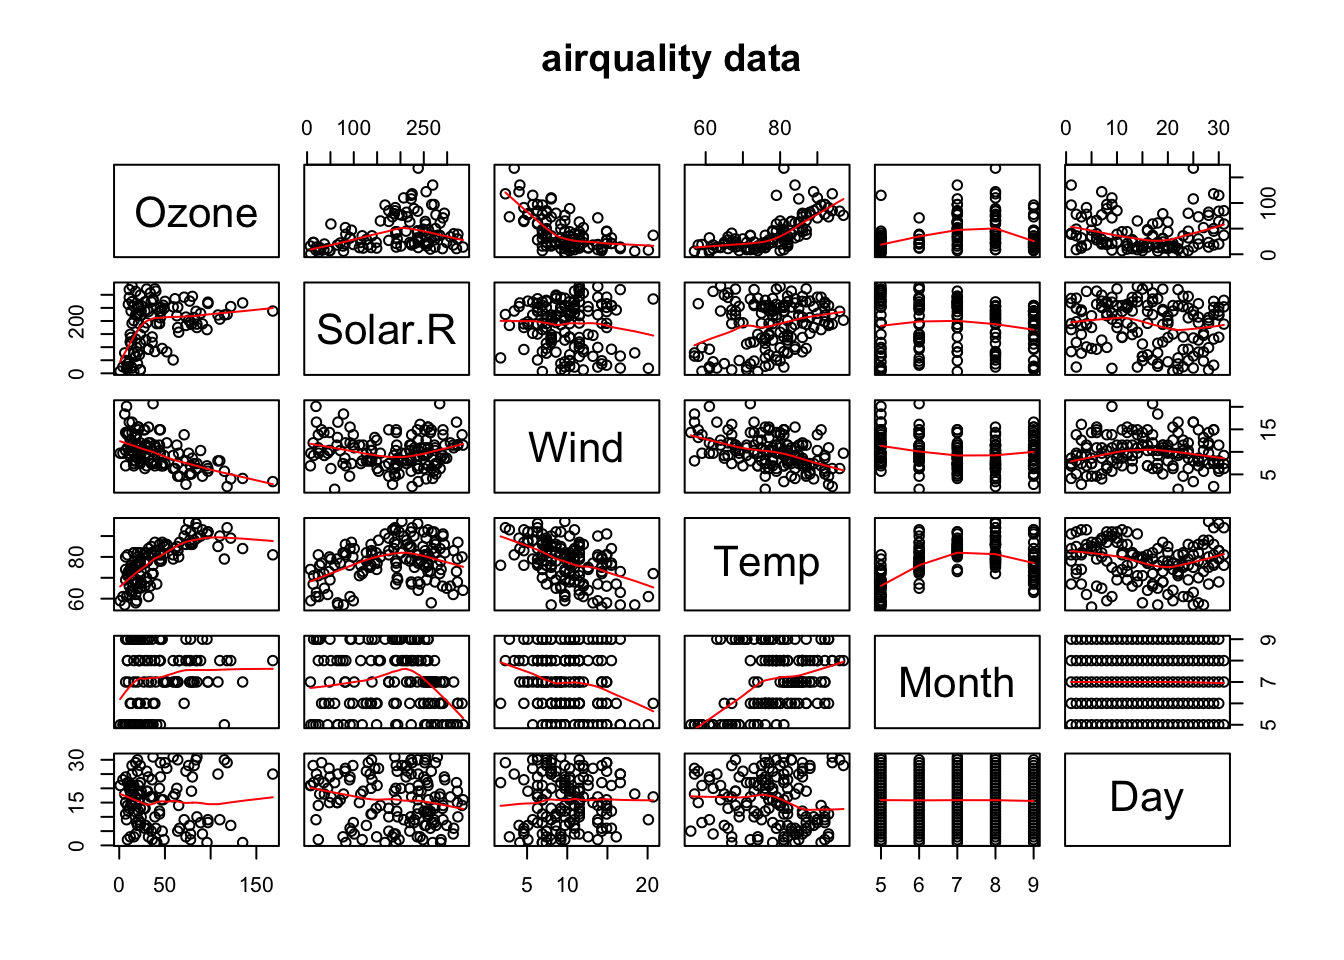
\includegraphics{cursoR_Euskaltel_files/figure-latex/unnamed-chunk-58-1.pdf}

\begin{Shaded}
\begin{Highlighting}[]
\NormalTok{ok <-}\StringTok{ }\KeywordTok{complete.cases}\NormalTok{(airquality)}
\NormalTok{airquality[ok,]}
\end{Highlighting}
\end{Shaded}

\section{Trabajando con data frames}\label{trabajando-con-data-frames-1}

\begin{itemize}
\tightlist
\item
  Los data frame se utilizand para guardas tablas de datos. Contiene
  elementos de la misma longitud.
\end{itemize}

\begin{Shaded}
\begin{Highlighting}[]
\NormalTok{mtcars}
\NormalTok{?mtcars       }\CommentTok{# help(mtcars)}
\end{Highlighting}
\end{Shaded}

\begin{itemize}
\tightlist
\item
  Observemos las primeras filas
\end{itemize}

\begin{Shaded}
\begin{Highlighting}[]
\KeywordTok{head}\NormalTok{(mtcars)}
\end{Highlighting}
\end{Shaded}

\begin{verbatim}
##                    mpg cyl disp  hp drat    wt  qsec vs am gear carb
## Mazda RX4         21.0   6  160 110 3.90 2.620 16.46  0  1    4    4
## Mazda RX4 Wag     21.0   6  160 110 3.90 2.875 17.02  0  1    4    4
## Datsun 710        22.8   4  108  93 3.85 2.320 18.61  1  1    4    1
## Hornet 4 Drive    21.4   6  258 110 3.08 3.215 19.44  1  0    3    1
## Hornet Sportabout 18.7   8  360 175 3.15 3.440 17.02  0  0    3    2
## Valiant           18.1   6  225 105 2.76 3.460 20.22  1  0    3    1
\end{verbatim}

\begin{itemize}
\tightlist
\item
  Estructura de un data frame
\end{itemize}

\begin{Shaded}
\begin{Highlighting}[]
\KeywordTok{str}\NormalTok{(mtcars) }\CommentTok{# visualiza la estructura del marco de datos}
\end{Highlighting}
\end{Shaded}

\begin{verbatim}
## 'data.frame':    32 obs. of  11 variables:
##  $ mpg : num  21 21 22.8 21.4 18.7 18.1 14.3 24.4 22.8 19.2 ...
##  $ cyl : num  6 6 4 6 8 6 8 4 4 6 ...
##  $ disp: num  160 160 108 258 360 ...
##  $ hp  : num  110 110 93 110 175 105 245 62 95 123 ...
##  $ drat: num  3.9 3.9 3.85 3.08 3.15 2.76 3.21 3.69 3.92 3.92 ...
##  $ wt  : num  2.62 2.88 2.32 3.21 3.44 ...
##  $ qsec: num  16.5 17 18.6 19.4 17 ...
##  $ vs  : num  0 0 1 1 0 1 0 1 1 1 ...
##  $ am  : num  1 1 1 0 0 0 0 0 0 0 ...
##  $ gear: num  4 4 4 3 3 3 3 4 4 4 ...
##  $ carb: num  4 4 1 1 2 1 4 2 2 4 ...
\end{verbatim}

\begin{itemize}
\tightlist
\item
  Select a car model:
\end{itemize}

\begin{Shaded}
\begin{Highlighting}[]
\NormalTok{mtcars[}\StringTok{"Mazda RX4"}\NormalTok{,] }\CommentTok{# usando nombres de las filas y las columnas}
\end{Highlighting}
\end{Shaded}

\begin{verbatim}
##           mpg cyl disp  hp drat   wt  qsec vs am gear carb
## Mazda RX4  21   6  160 110  3.9 2.62 16.46  0  1    4    4
\end{verbatim}

\begin{Shaded}
\begin{Highlighting}[]
\NormalTok{mtcars[}\KeywordTok{c}\NormalTok{(}\StringTok{"Datsun 710"}\NormalTok{, }\StringTok{"Camaro Z28"}\NormalTok{),] }
\end{Highlighting}
\end{Shaded}

\begin{verbatim}
##             mpg cyl disp  hp drat   wt  qsec vs am gear carb
## Datsun 710 22.8   4  108  93 3.85 2.32 18.61  1  1    4    1
## Camaro Z28 13.3   8  350 245 3.73 3.84 15.41  0  0    3    4
\end{verbatim}

\begin{itemize}
\tightlist
\item
  O variables concretas
\end{itemize}

\begin{Shaded}
\begin{Highlighting}[]
\NormalTok{mtcars[,}\KeywordTok{c}\NormalTok{(}\StringTok{"mpg"}\NormalTok{,}\StringTok{"am"}\NormalTok{)]}
\end{Highlighting}
\end{Shaded}

\begin{verbatim}
##                      mpg am
## Mazda RX4           21.0  1
## Mazda RX4 Wag       21.0  1
## Datsun 710          22.8  1
## Hornet 4 Drive      21.4  0
## Hornet Sportabout   18.7  0
## Valiant             18.1  0
## Duster 360          14.3  0
## Merc 240D           24.4  0
## Merc 230            22.8  0
## Merc 280            19.2  0
## Merc 280C           17.8  0
## Merc 450SE          16.4  0
## Merc 450SL          17.3  0
## Merc 450SLC         15.2  0
## Cadillac Fleetwood  10.4  0
## Lincoln Continental 10.4  0
## Chrysler Imperial   14.7  0
## Fiat 128            32.4  1
## Honda Civic         30.4  1
## Toyota Corolla      33.9  1
## Toyota Corona       21.5  0
## Dodge Challenger    15.5  0
## AMC Javelin         15.2  0
## Camaro Z28          13.3  0
## Pontiac Firebird    19.2  0
## Fiat X1-9           27.3  1
## Porsche 914-2       26.0  1
## Lotus Europa        30.4  1
## Ford Pantera L      15.8  1
## Ferrari Dino        19.7  1
## Maserati Bora       15.0  1
## Volvo 142E          21.4  1
\end{verbatim}

\begin{Shaded}
\begin{Highlighting}[]
\KeywordTok{library}\NormalTok{(psych)}
\KeywordTok{describe}\NormalTok{(mtcars)}
\end{Highlighting}
\end{Shaded}

\begin{verbatim}
##                                                    25%        50% 
##  352.00000   39.60853   84.20792    0.00000    2.42875    4.00000 
##        75%                       
##   18.97500  472.00000 -341.00000
\end{verbatim}

\chapter{\texorpdfstring{Análisis de datos básico en
\texttt{R}}{Análisis de datos básico en R}}\label{basic}

\section{Gráficos sencillos}\label{graficos-sencillos}

\begin{itemize}
\tightlist
\item
  Scatterplot
\end{itemize}

\begin{Shaded}
\begin{Highlighting}[]
\KeywordTok{attach}\NormalTok{(mtcars)}
\end{Highlighting}
\end{Shaded}

\begin{verbatim}
## The following objects are masked from mtcars (pos = 6):
## 
##     am, carb, cyl, disp, drat, gear, hp, mpg, qsec, vs, wt
\end{verbatim}

\begin{verbatim}
## The following object is masked from package:ggplot2:
## 
##     mpg
\end{verbatim}

\begin{verbatim}
## The following objects are masked from mtcars (pos = 26):
## 
##     am, carb, cyl, disp, drat, gear, hp, mpg, qsec, vs, wt
\end{verbatim}

\begin{Shaded}
\begin{Highlighting}[]
\KeywordTok{plot}\NormalTok{(wt, mpg, }\DataTypeTok{main=}\StringTok{"Scatterplot Example"}\NormalTok{,}
   \DataTypeTok{xlab=}\StringTok{"Car Weight "}\NormalTok{, }\DataTypeTok{ylab=}\StringTok{"Miles Per Gallon "}\NormalTok{, }\DataTypeTok{pch=}\DecValTok{19}\NormalTok{) }
\end{Highlighting}
\end{Shaded}

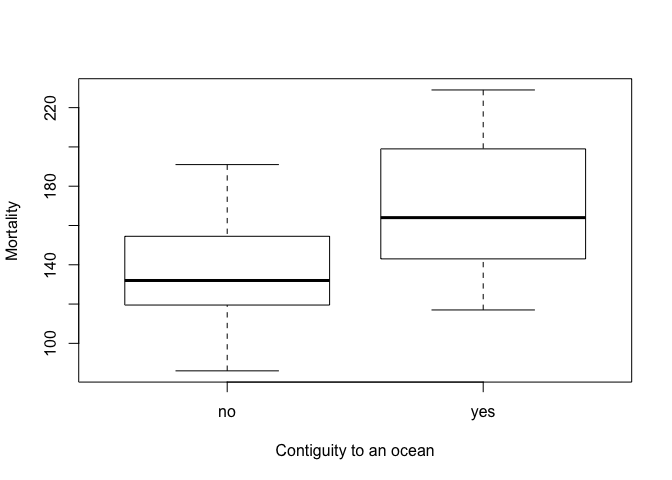
\includegraphics{cursoR_Euskaltel_files/figure-latex/unnamed-chunk-65-1.pdf}

\begin{itemize}
\tightlist
\item
  Matriz scatterplot
\end{itemize}

\begin{Shaded}
\begin{Highlighting}[]
\KeywordTok{pairs}\NormalTok{(}\OperatorTok{~}\NormalTok{mpg}\OperatorTok{+}\NormalTok{disp}\OperatorTok{+}\NormalTok{drat}\OperatorTok{+}\NormalTok{wt,}\DataTypeTok{data=}\NormalTok{mtcars,}
   \DataTypeTok{main=}\StringTok{"Simple Scatterplot Matrix"}\NormalTok{)}
\end{Highlighting}
\end{Shaded}

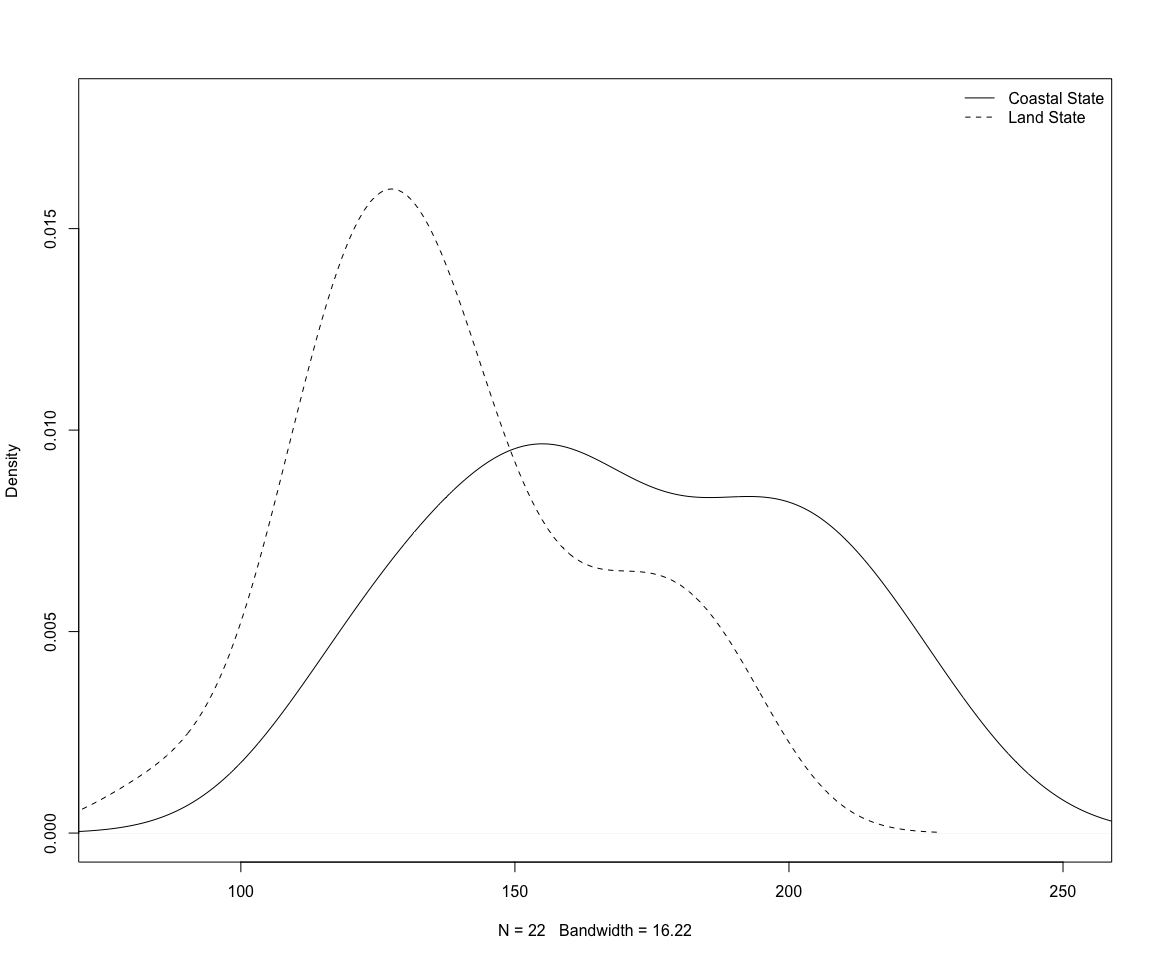
\includegraphics{cursoR_Euskaltel_files/figure-latex/unnamed-chunk-66-1.pdf}

\begin{itemize}
\tightlist
\item
  Barplot o diagrama de barras
\end{itemize}

\begin{Shaded}
\begin{Highlighting}[]
\NormalTok{tab <-}\StringTok{ }\KeywordTok{table}\NormalTok{(mtcars[,}\KeywordTok{c}\NormalTok{(}\StringTok{"cyl"}\NormalTok{)])}
\KeywordTok{barplot}\NormalTok{(tab)}
\end{Highlighting}
\end{Shaded}

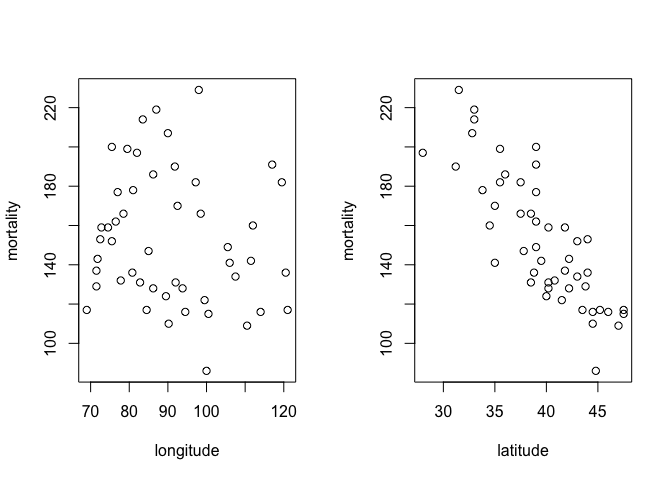
\includegraphics{cursoR_Euskaltel_files/figure-latex/unnamed-chunk-67-1.pdf}

\begin{itemize}
\tightlist
\item
  Piechart o diagrama de tarta
\end{itemize}

\begin{Shaded}
\begin{Highlighting}[]
\KeywordTok{pie}\NormalTok{(tab)}
\end{Highlighting}
\end{Shaded}

\begin{center}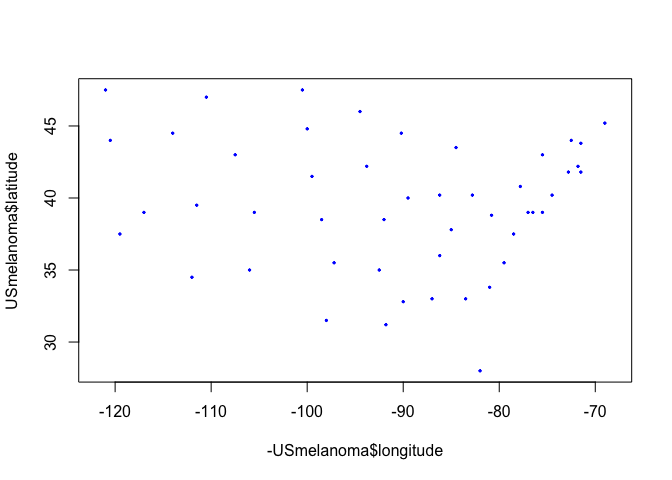
\includegraphics{cursoR_Euskaltel_files/figure-latex/unnamed-chunk-68-1} \end{center}

\textbf{Ejercicio:}

\begin{enumerate}
\def\labelenumi{\arabic{enumi}.}
\tightlist
\item
  El \texttt{data.frame} \texttt{VADeaths} contiene las tasas de
  mortalidad por cada 1000 habitantes en Virginia (EEUU) en 1940
\end{enumerate}

\begin{itemize}
\tightlist
\item
  Las tasas de mortalidad se miden cada 1000 habitantes por año. Se
  encuentran clasificadas por grupo de edad (filas) y grupo de población
  (columnas). Los grupos de edad son: 50-54, 55-59, 60-64, 65-69, 70-74
  y los grupos de población: \texttt{Rural/Male}, \texttt{Rural/Female},
  \texttt{Urban/Male} and \texttt{Urban/Female}.
\end{itemize}

\begin{Shaded}
\begin{Highlighting}[]
\KeywordTok{data}\NormalTok{(VADeaths)}
\NormalTok{VADeaths}
\end{Highlighting}
\end{Shaded}

\begin{verbatim}
##       Rural Male Rural Female Urban Male Urban Female
## 50-54       11.7          8.7       15.4          8.4
## 55-59       18.1         11.7       24.3         13.6
## 60-64       26.9         20.3       37.0         19.3
## 65-69       41.0         30.9       54.6         35.1
## 70-74       66.0         54.3       71.1         50.0
\end{verbatim}

\begin{itemize}
\item
  Calcula la media para cada grupo de edad.

  \begin{itemize}
  \tightlist
  \item
    \textbf{Result:}
  \end{itemize}
\end{itemize}

\begin{verbatim}
##  50-54  55-59  60-64  65-69  70-74 
## 11.050 16.925 25.875 40.400 60.350
\end{verbatim}

\begin{itemize}
\item
  Calcula la media para cada grupo de población.

  \begin{itemize}
  \tightlist
  \item
    \textbf{Resultado:}
  \end{itemize}
\end{itemize}

\begin{verbatim}
##   Rural Male Rural Female   Urban Male Urban Female 
##        32.74        25.18        40.48        25.28
\end{verbatim}

\begin{enumerate}
\def\labelenumi{\arabic{enumi}.}
\setcounter{enumi}{1}
\tightlist
\item
  El \texttt{data.frame} \texttt{rainforest} contiene diferentes
  variables de \texttt{species}
\end{enumerate}

\begin{Shaded}
\begin{Highlighting}[]
\KeywordTok{library}\NormalTok{(DAAG)}
\NormalTok{rainforest}
\NormalTok{?rainforest}
\KeywordTok{names}\NormalTok{(rainforest)}
\end{Highlighting}
\end{Shaded}

\begin{itemize}
\item
  Crear una tabla de conteos para cada \texttt{species} y realiza un
  gráfico descriptivo.

  \begin{itemize}
  \tightlist
  \item
    \textbf{Resultado:}
  \end{itemize}
\end{itemize}

\begin{verbatim}
## 
## Acacia mabellae      C. fraseri  Acmena smithii   B. myrtifolia 
##              16              12              26              11
\end{verbatim}

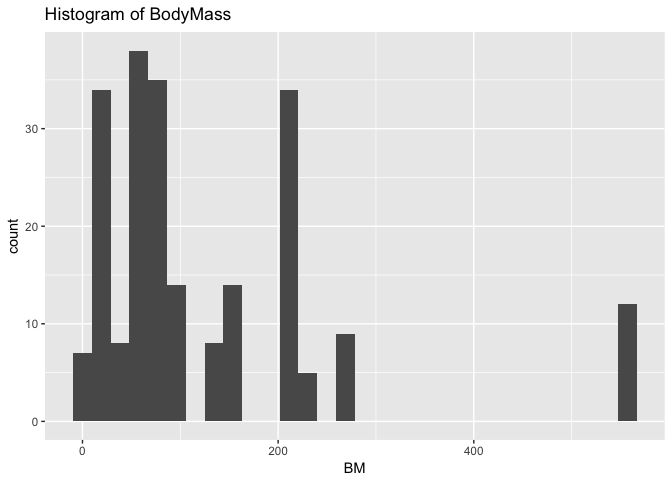
\includegraphics{cursoR_Euskaltel_files/figure-latex/unnamed-chunk-73-1.pdf}

\begin{enumerate}
\def\labelenumi{\arabic{enumi}.}
\setcounter{enumi}{2}
\tightlist
\item
  El \texttt{data.frame} \texttt{Acmena} est? creado a partir de
  \texttt{rainforest} mediante la función \texttt{subset}.
\end{enumerate}

\begin{itemize}
\tightlist
\item
  Realiza un gráfico que relacione la biomasa de la madera
  (\texttt{wood}) y el di?metro a la altura del pecho (\texttt{dbh}).
  Utiliza tambi?n la escala logarítmica.
\end{itemize}

\begin{Shaded}
\begin{Highlighting}[]
\NormalTok{Acmena <-}\StringTok{ }\KeywordTok{subset}\NormalTok{(rainforest, species }\OperatorTok{==}\StringTok{ "Acmena smithii"}\NormalTok{)}
\end{Highlighting}
\end{Shaded}

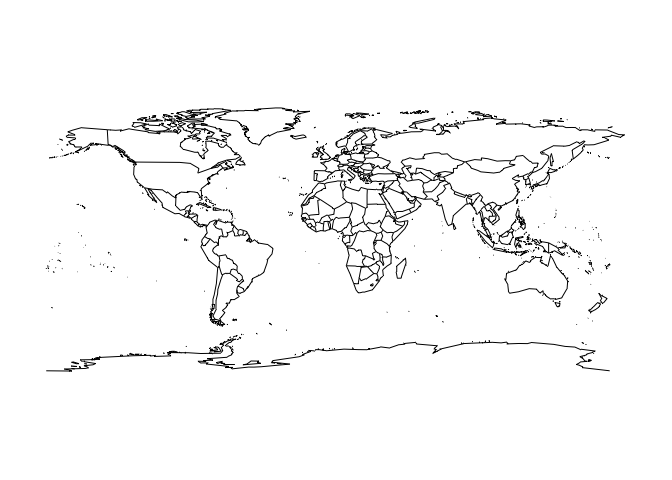
\includegraphics{cursoR_Euskaltel_files/figure-latex/unnamed-chunk-75-1.pdf}

\begin{itemize}
\tightlist
\item
  Calcula un histograma de la variable \texttt{dbh} mediante la función
  \texttt{hist}
\end{itemize}

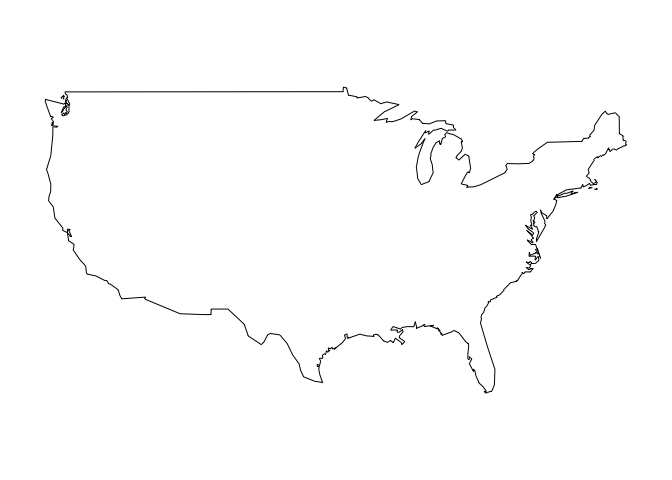
\includegraphics{cursoR_Euskaltel_files/figure-latex/unnamed-chunk-76-1.pdf}

\begin{enumerate}
\def\labelenumi{\arabic{enumi}.}
\setcounter{enumi}{3}
\item
  Crea un vector de n?meros enteros positivos impares the longitud 100 y
  calcula los valores entre 60 y 80.

  \begin{itemize}
  \tightlist
  \item
    \textbf{Result:}
  \end{itemize}
\end{enumerate}

\begin{verbatim}
##  [1] 61 63 65 67 69 71 73 75 77 79
\end{verbatim}

\begin{itemize}
\tightlist
\item
  \href{http://idaejin.github.io/bcam-courses/rbasics/rbasics_sol.R}{Soluciones
  aquí}
\end{itemize}

\begin{center}\rule{0.5\linewidth}{\linethickness}\end{center}

\section{Scatterplots}\label{scatterplots}

\begin{Shaded}
\begin{Highlighting}[]
\KeywordTok{library}\NormalTok{(MASS)}
\KeywordTok{data}\NormalTok{(}\StringTok{"mammals"}\NormalTok{)}
\NormalTok{?mammals}
\KeywordTok{head}\NormalTok{(mammals)}
\end{Highlighting}
\end{Shaded}

\begin{verbatim}
##                    body brain
## Arctic fox        3.385  44.5
## Owl monkey        0.480  15.5
## Mountain beaver   1.350   8.1
## Cow             465.000 423.0
## Grey wolf        36.330 119.5
## Goat             27.660 115.0
\end{verbatim}

\begin{Shaded}
\begin{Highlighting}[]
\KeywordTok{attach}\NormalTok{(mammals)}
\NormalTok{species <-}\StringTok{ }\KeywordTok{row.names}\NormalTok{(mammals)}
\NormalTok{x <-}\StringTok{ }\NormalTok{body}
\NormalTok{y <-}\StringTok{ }\NormalTok{brain}
\end{Highlighting}
\end{Shaded}

\begin{Shaded}
\begin{Highlighting}[]
\KeywordTok{library}\NormalTok{(calibrate)}
\CommentTok{# scatterplot}
\KeywordTok{plot}\NormalTok{(x,y, }\DataTypeTok{xlab =} \StringTok{"body weight in kgr"}\NormalTok{, }\DataTypeTok{ylab =} \StringTok{"brain weight in gr"}\NormalTok{, }
     \DataTypeTok{main=}\StringTok{"Body vs Brain weight }\CharTok{\textbackslash{}n}\StringTok{ for 62 Species of Land Mammals"}\NormalTok{,}\DataTypeTok{xlim=}\KeywordTok{c}\NormalTok{(}\DecValTok{0}\NormalTok{,}\DecValTok{8500}\NormalTok{))}
\KeywordTok{textxy}\NormalTok{(x,y,}\DataTypeTok{labs=}\NormalTok{species,}\DataTypeTok{col =} \StringTok{"blue"}\NormalTok{,}\DataTypeTok{cex=}\FloatTok{0.85}\NormalTok{) }
\end{Highlighting}
\end{Shaded}

\begin{center}\includegraphics{cursoR_Euskaltel_files/figure-latex/unnamed-chunk-79-1} \end{center}

Identificar un punto en el scatterplot

\begin{Shaded}
\begin{Highlighting}[]
\KeywordTok{identify}\NormalTok{(x,y,species)}
\end{Highlighting}
\end{Shaded}

En escala logarítmica

\begin{Shaded}
\begin{Highlighting}[]
\KeywordTok{plot}\NormalTok{(}\KeywordTok{log}\NormalTok{(x),}\KeywordTok{log}\NormalTok{(y), }\DataTypeTok{xlab =} \StringTok{"log body weight in kgr"}\NormalTok{, }\DataTypeTok{ylab =} \StringTok{"log brain weight in gr"}\NormalTok{, }
     \DataTypeTok{main=}\StringTok{"log Body vs log Brain weight }\CharTok{\textbackslash{}n}\StringTok{ for 62 Species of Land Mammals"}\NormalTok{)}
\KeywordTok{textxy}\NormalTok{(}\KeywordTok{log}\NormalTok{(x),}\KeywordTok{log}\NormalTok{(y),}\DataTypeTok{labs=}\NormalTok{species,}\DataTypeTok{col =} \StringTok{"blue"}\NormalTok{,}\DataTypeTok{cex=}\FloatTok{0.85}\NormalTok{) }
\end{Highlighting}
\end{Shaded}

\begin{center}\includegraphics{cursoR_Euskaltel_files/figure-latex/unnamed-chunk-81-1} \end{center}

Identificar un punto en la escala logarítmica

\begin{Shaded}
\begin{Highlighting}[]
\KeywordTok{identify}\NormalTok{(}\KeywordTok{log}\NormalTok{(x),}\KeywordTok{log}\NormalTok{(y),species)}
\end{Highlighting}
\end{Shaded}

\section{más opciones gráficas}\label{mas-opciones-graficas}

\textbf{Varios conjuntos de datos en un sólo gráfico}

Una vez realizado un \texttt{plot}, el comando \texttt{points} permite
aadir nuevas observaciones.

\begin{Shaded}
\begin{Highlighting}[]
\KeywordTok{set.seed}\NormalTok{(}\DecValTok{1234}\NormalTok{)}
\NormalTok{ x <-}\StringTok{ }\KeywordTok{rnorm}\NormalTok{(}\DecValTok{10}\NormalTok{,}\DataTypeTok{sd=}\DecValTok{5}\NormalTok{,}\DataTypeTok{mean=}\DecValTok{20}\NormalTok{)}
\NormalTok{ y <-}\StringTok{ }\FloatTok{2.5}\OperatorTok{*}\NormalTok{x }\OperatorTok{-}\StringTok{ }\FloatTok{1.0} \OperatorTok{+}\StringTok{ }\KeywordTok{rnorm}\NormalTok{(}\DecValTok{10}\NormalTok{,}\DataTypeTok{sd=}\DecValTok{9}\NormalTok{,}\DataTypeTok{mean=}\DecValTok{0}\NormalTok{)}
 \KeywordTok{cor}\NormalTok{(x,y)}
\end{Highlighting}
\end{Shaded}

\begin{verbatim}
## [1] 0.7512194
\end{verbatim}

\begin{Shaded}
\begin{Highlighting}[]
 \KeywordTok{plot}\NormalTok{(x,y,}\DataTypeTok{xlab=}\StringTok{"Independent"}\NormalTok{,}\DataTypeTok{ylab=}\StringTok{"Dependent"}\NormalTok{,}\DataTypeTok{main=}\StringTok{"Random plot"}\NormalTok{)}
\NormalTok{ x1 <-}\StringTok{ }\KeywordTok{runif}\NormalTok{(}\DecValTok{8}\NormalTok{,}\DecValTok{15}\NormalTok{,}\DecValTok{25}\NormalTok{)}
\NormalTok{ y1 <-}\StringTok{ }\FloatTok{2.5}\OperatorTok{*}\NormalTok{x1 }\OperatorTok{-}\StringTok{ }\FloatTok{1.0} \OperatorTok{+}\StringTok{ }\KeywordTok{runif}\NormalTok{(}\DecValTok{8}\NormalTok{,}\OperatorTok{-}\DecValTok{6}\NormalTok{,}\DecValTok{6}\NormalTok{)}
 \KeywordTok{points}\NormalTok{(x1,y1,}\DataTypeTok{col=}\DecValTok{2}\NormalTok{)}
\end{Highlighting}
\end{Shaded}

\includegraphics{cursoR_Euskaltel_files/figure-latex/unnamed-chunk-83-1.pdf}

con la leyenda

\begin{Shaded}
\begin{Highlighting}[]
\KeywordTok{set.seed}\NormalTok{(}\DecValTok{1234}\NormalTok{)}
\NormalTok{x2 <-}\StringTok{ }\KeywordTok{runif}\NormalTok{(}\DecValTok{8}\NormalTok{,}\DecValTok{15}\NormalTok{,}\DecValTok{25}\NormalTok{)}
\NormalTok{y2 <-}\StringTok{ }\FloatTok{2.5}\OperatorTok{*}\NormalTok{x2 }\OperatorTok{-}\StringTok{ }\FloatTok{1.0} \OperatorTok{+}\StringTok{ }\KeywordTok{runif}\NormalTok{(}\DecValTok{8}\NormalTok{,}\OperatorTok{-}\DecValTok{6}\NormalTok{,}\DecValTok{6}\NormalTok{)}
 \KeywordTok{plot}\NormalTok{(x,y,}\DataTypeTok{xlab=}\StringTok{"Independent"}\NormalTok{,}\DataTypeTok{ylab=}\StringTok{"Dependent"}\NormalTok{,}\DataTypeTok{main=}\StringTok{"Random plot"}\NormalTok{)}
 \KeywordTok{points}\NormalTok{(x1,y1,}\DataTypeTok{col=}\DecValTok{2}\NormalTok{,}\DataTypeTok{pch=}\DecValTok{3}\NormalTok{)}
 \KeywordTok{points}\NormalTok{(x2,y2,}\DataTypeTok{col=}\DecValTok{4}\NormalTok{,}\DataTypeTok{pch=}\DecValTok{5}\NormalTok{)}
 \KeywordTok{legend}\NormalTok{(}\StringTok{"topleft"}\NormalTok{,}\KeywordTok{c}\NormalTok{(}\StringTok{"Original"}\NormalTok{,}\StringTok{"one"}\NormalTok{,}\StringTok{"two"}\NormalTok{),}\DataTypeTok{col=}\KeywordTok{c}\NormalTok{(}\DecValTok{1}\NormalTok{,}\DecValTok{2}\NormalTok{,}\DecValTok{4}\NormalTok{),}\DataTypeTok{pch=}\KeywordTok{c}\NormalTok{(}\DecValTok{1}\NormalTok{,}\DecValTok{3}\NormalTok{,}\DecValTok{5}\NormalTok{))}
\end{Highlighting}
\end{Shaded}

\includegraphics{cursoR_Euskaltel_files/figure-latex/unnamed-chunk-84-1.pdf}

\textbf{Varios gráficos en un sola imagen}

\begin{Shaded}
\begin{Highlighting}[]
\KeywordTok{set.seed}\NormalTok{(}\DecValTok{1234}\NormalTok{)}
 \KeywordTok{par}\NormalTok{(}\DataTypeTok{mfrow=}\KeywordTok{c}\NormalTok{(}\DecValTok{2}\NormalTok{,}\DecValTok{3}\NormalTok{))}
 \KeywordTok{boxplot}\NormalTok{(}\KeywordTok{rnorm}\NormalTok{(}\DecValTok{100}\NormalTok{),}\DataTypeTok{main=}\StringTok{"first plot"}\NormalTok{)}
 \KeywordTok{boxplot}\NormalTok{(}\KeywordTok{rgamma}\NormalTok{(}\DecValTok{100}\NormalTok{,}\DecValTok{2}\NormalTok{),}\DataTypeTok{main=}\StringTok{"second plot"}\NormalTok{, }\DataTypeTok{horizontal=}\OtherTok{TRUE}\NormalTok{,}\DataTypeTok{col=}\StringTok{"bisque"}\NormalTok{)}
 \KeywordTok{plot}\NormalTok{(}\KeywordTok{rnorm}\NormalTok{(}\DecValTok{100}\NormalTok{),}\DataTypeTok{xlab=}\StringTok{"third plot"}\NormalTok{,}
      \DataTypeTok{ylab=}\StringTok{"y-label"}\NormalTok{,}\DataTypeTok{main=}\StringTok{"x-label"}\NormalTok{)}
 \KeywordTok{hist}\NormalTok{(}\KeywordTok{rnorm}\NormalTok{(}\DecValTok{100}\NormalTok{),}\DataTypeTok{main=}\StringTok{"fourth plot"}\NormalTok{,}\DataTypeTok{col=}\StringTok{"lightgrey"}\NormalTok{)}
 \KeywordTok{hist}\NormalTok{(}\KeywordTok{rexp}\NormalTok{(}\DecValTok{100}\NormalTok{),}\DataTypeTok{main=}\StringTok{"fifth plot"}\NormalTok{,}\DataTypeTok{col=}\StringTok{"blue"}\NormalTok{)}
 \KeywordTok{plot}\NormalTok{(}\KeywordTok{rnorm}\NormalTok{(}\DecValTok{100}\NormalTok{),}\KeywordTok{rexp}\NormalTok{(}\DecValTok{100}\NormalTok{),}\DataTypeTok{main=}\StringTok{"sixth plot"}\NormalTok{)}
\end{Highlighting}
\end{Shaded}

\includegraphics{cursoR_Euskaltel_files/figure-latex/unnamed-chunk-85-1.pdf}

\textbf{Relaciones entre variables}

\begin{Shaded}
\begin{Highlighting}[]
\NormalTok{uData <-}\StringTok{ }\KeywordTok{rnorm}\NormalTok{(}\DecValTok{20}\NormalTok{)}
\NormalTok{vData <-}\StringTok{ }\KeywordTok{rnorm}\NormalTok{(}\DecValTok{20}\NormalTok{,}\DataTypeTok{mean=}\DecValTok{5}\NormalTok{)}
\NormalTok{wData <-}\StringTok{ }\NormalTok{uData }\OperatorTok{+}\StringTok{ }\DecValTok{2}\OperatorTok{*}\NormalTok{vData }\OperatorTok{+}\StringTok{ }\KeywordTok{rnorm}\NormalTok{(}\DecValTok{20}\NormalTok{,}\DataTypeTok{sd=}\FloatTok{0.5}\NormalTok{)}
\NormalTok{xData <-}\StringTok{ }\OperatorTok{-}\DecValTok{2}\OperatorTok{*}\NormalTok{uData}\OperatorTok{+}\KeywordTok{rnorm}\NormalTok{(}\DecValTok{20}\NormalTok{,}\DataTypeTok{sd=}\FloatTok{0.1}\NormalTok{)}
\NormalTok{yData <-}\StringTok{  }\DecValTok{3}\OperatorTok{*}\NormalTok{vData}\OperatorTok{+}\KeywordTok{rnorm}\NormalTok{(}\DecValTok{20}\NormalTok{,}\DataTypeTok{sd=}\FloatTok{2.5}\NormalTok{)}
\NormalTok{d <-}\StringTok{ }\KeywordTok{data.frame}\NormalTok{(}\DataTypeTok{u=}\NormalTok{uData,}\DataTypeTok{v=}\NormalTok{vData,}\DataTypeTok{w=}\NormalTok{wData,}\DataTypeTok{x=}\NormalTok{xData,}\DataTypeTok{y=}\NormalTok{yData)}
\KeywordTok{pairs}\NormalTok{(d)}
\end{Highlighting}
\end{Shaded}

\includegraphics{cursoR_Euskaltel_files/figure-latex/unnamed-chunk-86-1.pdf}

\textbf{Gráfico de correlaciones}

La función \texttt{corrplot} de la librer?a \texttt{corrplot} permite
visualizar una matriz de correlaciones calculada mediante la función
\texttt{cor}

\begin{Shaded}
\begin{Highlighting}[]
\KeywordTok{library}\NormalTok{(corrplot)}
\NormalTok{M <-}\StringTok{ }\KeywordTok{cor}\NormalTok{(d)}
\KeywordTok{corrplot}\NormalTok{(M, }\DataTypeTok{method=}\StringTok{"circle"}\NormalTok{,}\DataTypeTok{type=}\StringTok{"upper"}\NormalTok{)}
\end{Highlighting}
\end{Shaded}

\includegraphics{cursoR_Euskaltel_files/figure-latex/unnamed-chunk-87-1.pdf}

\textbf{Gráficos de superficies: \texttt{image}, \texttt{contour} y
\texttt{persp}}

\begin{Shaded}
\begin{Highlighting}[]
\NormalTok{x <-}\StringTok{ }\KeywordTok{seq}\NormalTok{(}\DecValTok{0}\NormalTok{,}\DecValTok{2}\OperatorTok{*}\NormalTok{pi,}\DataTypeTok{by=}\NormalTok{pi}\OperatorTok{/}\DecValTok{50}\NormalTok{)}
\NormalTok{y <-}\StringTok{ }\NormalTok{x}
\NormalTok{xg <-}\StringTok{ }\NormalTok{(x}\OperatorTok{*}\DecValTok{0}\OperatorTok{+}\DecValTok{1}\NormalTok{) }\OperatorTok\StringTok{ }\KeywordTok{t}\NormalTok{(y)}
\NormalTok{yg <-}\StringTok{ }\NormalTok{(x) }\OperatorTok\StringTok{ }\KeywordTok{t}\NormalTok{(y}\OperatorTok{*}\DecValTok{0}\OperatorTok{+}\DecValTok{1}\NormalTok{)}
\NormalTok{f <-}\StringTok{ }\KeywordTok{sin}\NormalTok{(xg}\OperatorTok{*}\NormalTok{yg)}

\KeywordTok{par}\NormalTok{(}\DataTypeTok{mfrow=}\KeywordTok{c}\NormalTok{(}\DecValTok{2}\NormalTok{,}\DecValTok{2}\NormalTok{))}
\KeywordTok{image}\NormalTok{(x,y,f)}
\KeywordTok{contour}\NormalTok{(x,y,f)}
\KeywordTok{contour}\NormalTok{(x,y,f,}\DataTypeTok{nlevels=}\DecValTok{4}\NormalTok{)}
\KeywordTok{image}\NormalTok{(x,y,f,}\DataTypeTok{col=}\KeywordTok{grey.colors}\NormalTok{(}\DecValTok{100}\NormalTok{))}
\KeywordTok{contour}\NormalTok{(x,y,f,}\DataTypeTok{nlevels=}\DecValTok{4}\NormalTok{,}\DataTypeTok{add=}\OtherTok{TRUE}\NormalTok{,}\DataTypeTok{col=}\StringTok{"red"}\NormalTok{)}
\end{Highlighting}
\end{Shaded}

\includegraphics{cursoR_Euskaltel_files/figure-latex/unnamed-chunk-88-1.pdf}

Podemos utilizar la función \texttt{persp}

\begin{Shaded}
\begin{Highlighting}[]
\KeywordTok{persp}\NormalTok{(x,y,f,}\DataTypeTok{theta=}\OperatorTok{-}\DecValTok{30}\NormalTok{,}\DataTypeTok{phi=}\DecValTok{55}\NormalTok{,}\DataTypeTok{col=}\StringTok{"lightgrey"}\NormalTok{,}\DataTypeTok{shade=}\NormalTok{.}\DecValTok{01}\NormalTok{)}
\end{Highlighting}
\end{Shaded}

\begin{center}\includegraphics{cursoR_Euskaltel_files/figure-latex/unnamed-chunk-89-1} \end{center}

o representar im?genes

\begin{Shaded}
\begin{Highlighting}[]
\KeywordTok{library}\NormalTok{(fields)}
\KeywordTok{data}\NormalTok{(lennon)}
\KeywordTok{image}\NormalTok{(lennon,}\DataTypeTok{col=}\KeywordTok{grey}\NormalTok{(}\KeywordTok{seq}\NormalTok{(}\DecValTok{0}\NormalTok{,}\DecValTok{1}\NormalTok{,}\DataTypeTok{l=}\DecValTok{256}\NormalTok{)))}
\end{Highlighting}
\end{Shaded}

\includegraphics{cursoR_Euskaltel_files/figure-latex/unnamed-chunk-90-1.pdf}

\section{Tablas de clasificación cruzada o de
contigencia}\label{tablas-de-clasificacion-cruzada-o-de-contigencia}

\begin{Shaded}
\begin{Highlighting}[]
\KeywordTok{library}\NormalTok{(MASS)}
\KeywordTok{data}\NormalTok{(quine)}
\KeywordTok{head}\NormalTok{(quine)}
\end{Highlighting}
\end{Shaded}

\begin{verbatim}
##   Eth Sex Age Lrn Days
## 1   A   M  F0  SL    2
## 2   A   M  F0  SL   11
## 3   A   M  F0  SL   14
## 4   A   M  F0  AL    5
## 5   A   M  F0  AL    5
## 6   A   M  F0  AL   13
\end{verbatim}

\begin{Shaded}
\begin{Highlighting}[]
\KeywordTok{attach}\NormalTok{(quine)}
\end{Highlighting}
\end{Shaded}

\begin{verbatim}
## The following objects are masked from quine (pos = 6):
## 
##     Age, Days, Eth, Lrn, Sex
\end{verbatim}

\begin{verbatim}
## The following objects are masked from quine (pos = 18):
## 
##     Age, Days, Eth, Lrn, Sex
\end{verbatim}

\begin{Shaded}
\begin{Highlighting}[]
\KeywordTok{table}\NormalTok{(Sex)}
\end{Highlighting}
\end{Shaded}

\begin{verbatim}
## Sex
##  F  M 
## 80 66
\end{verbatim}

\begin{Shaded}
\begin{Highlighting}[]
\KeywordTok{table}\NormalTok{(Sex,Age)}
\end{Highlighting}
\end{Shaded}

\begin{verbatim}
##    Age
## Sex F0 F1 F2 F3
##   F 10 32 19 19
##   M 17 14 21 14
\end{verbatim}

\begin{Shaded}
\begin{Highlighting}[]
\CommentTok{# or xtabs}
\KeywordTok{xtabs}\NormalTok{(}\OperatorTok{~}\NormalTok{Sex}\OperatorTok{+}\NormalTok{Age,}\DataTypeTok{data=}\NormalTok{quine)}
\end{Highlighting}
\end{Shaded}

\begin{verbatim}
##    Age
## Sex F0 F1 F2 F3
##   F 10 32 19 19
##   M 17 14 21 14
\end{verbatim}

\begin{Shaded}
\begin{Highlighting}[]
\KeywordTok{xtabs}\NormalTok{(}\OperatorTok{~}\NormalTok{Sex}\OperatorTok{+}\NormalTok{Age}\OperatorTok{+}\NormalTok{Eth,}\DataTypeTok{data=}\NormalTok{quine)}
\end{Highlighting}
\end{Shaded}

\begin{verbatim}
## , , Eth = A
## 
##    Age
## Sex F0 F1 F2 F3
##   F  5 15  9  9
##   M  8  5 11  7
## 
## , , Eth = N
## 
##    Age
## Sex F0 F1 F2 F3
##   F  5 17 10 10
##   M  9  9 10  7
\end{verbatim}

\section{cálculos sobre tablas de
contigencia}\label{calculos-sobre-tablas-de-contigencia}

\begin{Shaded}
\begin{Highlighting}[]
\KeywordTok{tapply}\NormalTok{(Days,Age,mean)}
\end{Highlighting}
\end{Shaded}

\begin{verbatim}
##       F0       F1       F2       F3 
## 14.85185 11.15217 21.05000 19.60606
\end{verbatim}

\begin{Shaded}
\begin{Highlighting}[]
\KeywordTok{tapply}\NormalTok{(Days,}\KeywordTok{list}\NormalTok{(Sex,Age),mean)}
\end{Highlighting}
\end{Shaded}

\begin{verbatim}
##         F0       F1       F2       F3
## F 18.70000 12.96875 18.42105 14.00000
## M 12.58824  7.00000 23.42857 27.21429
\end{verbatim}

\begin{Shaded}
\begin{Highlighting}[]
\KeywordTok{tapply}\NormalTok{(Days,}\KeywordTok{list}\NormalTok{(Sex,Age),}\ControlFlowTok{function}\NormalTok{(x) }\KeywordTok{sqrt}\NormalTok{(}\KeywordTok{var}\NormalTok{(x)}\OperatorTok{/}\KeywordTok{length}\NormalTok{(x)))}
\end{Highlighting}
\end{Shaded}

\begin{verbatim}
##         F0       F1       F2       F3
## F 4.208589 2.329892 5.299959 2.940939
## M 3.768151 1.418093 3.766122 4.569582
\end{verbatim}

\section{Datos cualitativos}\label{datos-cualitativos}

Supongamos unos datos cualquiera de las variables \texttt{treatment} y
\texttt{improvement} de pacientes a una enfermedad determinada.

\begin{Shaded}
\begin{Highlighting}[]
\NormalTok{treatment <-}\StringTok{ }\KeywordTok{factor}\NormalTok{(}\KeywordTok{rep}\NormalTok{(}\KeywordTok{c}\NormalTok{(}\DecValTok{1}\NormalTok{, }\DecValTok{2}\NormalTok{), }\KeywordTok{c}\NormalTok{(}\DecValTok{43}\NormalTok{, }\DecValTok{41}\NormalTok{)), }\DataTypeTok{levels =} \KeywordTok{c}\NormalTok{(}\DecValTok{1}\NormalTok{, }\DecValTok{2}\NormalTok{),}
                    \DataTypeTok{labels =} \KeywordTok{c}\NormalTok{(}\StringTok{"placebo"}\NormalTok{, }\StringTok{"treated"}\NormalTok{))}
\NormalTok{improved <-}\StringTok{ }\KeywordTok{factor}\NormalTok{(}\KeywordTok{rep}\NormalTok{(}\KeywordTok{c}\NormalTok{(}\DecValTok{1}\NormalTok{, }\DecValTok{2}\NormalTok{, }\DecValTok{3}\NormalTok{, }\DecValTok{1}\NormalTok{, }\DecValTok{2}\NormalTok{, }\DecValTok{3}\NormalTok{), }\KeywordTok{c}\NormalTok{(}\DecValTok{29}\NormalTok{, }\DecValTok{7}\NormalTok{, }\DecValTok{7}\NormalTok{, }\DecValTok{13}\NormalTok{, }\DecValTok{7}\NormalTok{, }\DecValTok{21}\NormalTok{)),}
                   \DataTypeTok{levels =} \KeywordTok{c}\NormalTok{(}\DecValTok{1}\NormalTok{, }\DecValTok{2}\NormalTok{, }\DecValTok{3}\NormalTok{),}
                   \DataTypeTok{labels =} \KeywordTok{c}\NormalTok{(}\StringTok{"none"}\NormalTok{, }\StringTok{"some"}\NormalTok{, }\StringTok{"marked"}\NormalTok{))}
\end{Highlighting}
\end{Shaded}

Tabla de contigencia

\begin{Shaded}
\begin{Highlighting}[]
\KeywordTok{xtabs}\NormalTok{(}\OperatorTok{~}\NormalTok{treatment}\OperatorTok{+}\NormalTok{improved)}
\end{Highlighting}
\end{Shaded}

\begin{verbatim}
##          improved
## treatment none some marked
##   placebo   29    7      7
##   treated   13    7     21
\end{verbatim}

De manera gráfica,

\begin{Shaded}
\begin{Highlighting}[]
\KeywordTok{spineplot}\NormalTok{(improved }\OperatorTok{~}\StringTok{ }\NormalTok{treatment)}
\end{Highlighting}
\end{Shaded}

\includegraphics{cursoR_Euskaltel_files/figure-latex/unnamed-chunk-97-1.pdf}

El conjunto de datos de \texttt{R}, \texttt{UCBAdmissions}contiene los
datos agregadps de los solicitantes a universidad de Berkeley a los seis
departamentos más grandes en 1973 clasificados por sexo y admisión.

\begin{Shaded}
\begin{Highlighting}[]
\KeywordTok{data}\NormalTok{(}\StringTok{"UCBAdmissions"}\NormalTok{)}
\NormalTok{?UCBAdmissions}
\KeywordTok{apply}\NormalTok{(UCBAdmissions, }\KeywordTok{c}\NormalTok{(}\DecValTok{2}\NormalTok{,}\DecValTok{1}\NormalTok{), sum)}
\end{Highlighting}
\end{Shaded}

\begin{verbatim}
##         Admit
## Gender   Admitted Rejected
##   Male       1198     1493
##   Female      557     1278
\end{verbatim}

\begin{Shaded}
\begin{Highlighting}[]
\KeywordTok{prop.table}\NormalTok{(}\KeywordTok{apply}\NormalTok{(UCBAdmissions, }\KeywordTok{c}\NormalTok{(}\DecValTok{2}\NormalTok{,}\DecValTok{1}\NormalTok{), sum))}
\end{Highlighting}
\end{Shaded}

\begin{verbatim}
##         Admit
## Gender    Admitted  Rejected
##   Male   0.2646929 0.3298719
##   Female 0.1230667 0.2823685
\end{verbatim}

\begin{Shaded}
\begin{Highlighting}[]
\KeywordTok{ftable}\NormalTok{(UCBAdmissions)}
\end{Highlighting}
\end{Shaded}

\begin{verbatim}
##                 Dept   A   B   C   D   E   F
## Admit    Gender                             
## Admitted Male        512 353 120 138  53  22
##          Female       89  17 202 131  94  24
## Rejected Male        313 207 205 279 138 351
##          Female       19   8 391 244 299 317
\end{verbatim}

Con \texttt{ftable} podemos presentar la información con mayor claridad

\begin{Shaded}
\begin{Highlighting}[]
\KeywordTok{ftable}\NormalTok{(}\KeywordTok{round}\NormalTok{(}\KeywordTok{prop.table}\NormalTok{(UCBAdmissions), }\DecValTok{3}\NormalTok{),}
       \DataTypeTok{row.vars=}\StringTok{"Dept"}\NormalTok{, }\DataTypeTok{col.vars =} \KeywordTok{c}\NormalTok{(}\StringTok{"Gender"}\NormalTok{, }\StringTok{"Admit"}\NormalTok{))}
\end{Highlighting}
\end{Shaded}

\begin{verbatim}
##      Gender     Male            Female         
##      Admit  Admitted Rejected Admitted Rejected
## Dept                                           
## A              0.113    0.069    0.020    0.004
## B              0.078    0.046    0.004    0.002
## C              0.027    0.045    0.045    0.086
## D              0.030    0.062    0.029    0.054
## E              0.012    0.030    0.021    0.066
## F              0.005    0.078    0.005    0.070
\end{verbatim}

Resulta más intereseante mostrar la información por género
\texttt{Gender} y \texttt{Dept} combinados (dimensiones 2 y 3 del
array). Nótese que las tasas de admisión por \texttt{male} y
\texttt{female} son más o menos similares en todos los departamentos,
excepto en ``A'', donde las tasas de las mujeres es mayor.

\begin{Shaded}
\begin{Highlighting}[]
\CommentTok{# prop.table(UCBAdmissions, c(2,3))}
\KeywordTok{ftable}\NormalTok{(}\KeywordTok{round}\NormalTok{(}\KeywordTok{prop.table}\NormalTok{(UCBAdmissions, }\KeywordTok{c}\NormalTok{(}\DecValTok{2}\NormalTok{,}\DecValTok{3}\NormalTok{)), }\DecValTok{2}\NormalTok{),}
       \DataTypeTok{row.vars=}\StringTok{"Dept"}\NormalTok{, }\DataTypeTok{col.vars =} \KeywordTok{c}\NormalTok{(}\StringTok{"Gender"}\NormalTok{, }\StringTok{"Admit"}\NormalTok{))}
\end{Highlighting}
\end{Shaded}

\begin{verbatim}
##      Gender     Male            Female         
##      Admit  Admitted Rejected Admitted Rejected
## Dept                                           
## A               0.62     0.38     0.82     0.18
## B               0.63     0.37     0.68     0.32
## C               0.37     0.63     0.34     0.66
## D               0.33     0.67     0.35     0.65
## E               0.28     0.72     0.24     0.76
## F               0.06     0.94     0.07     0.93
\end{verbatim}

\begin{Shaded}
\begin{Highlighting}[]
\NormalTok{## Data aggregated over departments}
\KeywordTok{apply}\NormalTok{(UCBAdmissions, }\KeywordTok{c}\NormalTok{(}\DecValTok{1}\NormalTok{, }\DecValTok{2}\NormalTok{), sum)}
\end{Highlighting}
\end{Shaded}

\begin{verbatim}
##           Gender
## Admit      Male Female
##   Admitted 1198    557
##   Rejected 1493   1278
\end{verbatim}

gr?ficamente

\begin{Shaded}
\begin{Highlighting}[]
\KeywordTok{spineplot}\NormalTok{(}\KeywordTok{margin.table}\NormalTok{(UCBAdmissions, }\KeywordTok{c}\NormalTok{(}\DecValTok{3}\NormalTok{, }\DecValTok{2}\NormalTok{)),}
           \DataTypeTok{main =} \StringTok{"Applications at UCB"}\NormalTok{)}
\end{Highlighting}
\end{Shaded}

\includegraphics{cursoR_Euskaltel_files/figure-latex/unnamed-chunk-102-1.pdf}

\begin{Shaded}
\begin{Highlighting}[]
\KeywordTok{spineplot}\NormalTok{(}\KeywordTok{margin.table}\NormalTok{(UCBAdmissions, }\KeywordTok{c}\NormalTok{(}\DecValTok{3}\NormalTok{, }\DecValTok{1}\NormalTok{)),}
           \DataTypeTok{main =} \StringTok{"Admissions at UCB"}\NormalTok{)}
\end{Highlighting}
\end{Shaded}

\includegraphics{cursoR_Euskaltel_files/figure-latex/unnamed-chunk-102-2.pdf}

Estos datos ilustran la denominada \emph{paradoja de Simpson}. Este
hecho ha sido analizado como un posible caso de discriminación por sexo
en las tasas de admisión en Berkeley. De los 2691 hombres que
solicitaron se admitidos, 1198 (44.5\%) fueron admitidos, comparado con
las 1835 mujeres de las cuales tan s?lo 557 (30.4\%) fueron admitidas.
Se podr?a por tanto concluir que los hombres tienes tasas de admisión
mayores que las mujeres.
\href{https://en.wikipedia.org/wiki/Simpson\%27s_paradox\#UC_Berkeley_gender_bias}{Wikipedia:
Gender Bias UC Berkeley}. See animation at
\href{http://vudlab.com/simpsons/}{link}

\section{Datos cuantitativos}\label{datos-cuantitativos}

\begin{Shaded}
\begin{Highlighting}[]
\KeywordTok{head}\NormalTok{(faithful)}
\end{Highlighting}
\end{Shaded}

\begin{verbatim}
##   eruptions waiting
## 1     3.600      79
## 2     1.800      54
## 3     3.333      74
## 4     2.283      62
## 5     4.533      85
## 6     2.883      55
\end{verbatim}

Consideremos los datos del geyse Old Faithful en el parque nacional de
Yellowstone, EEUU.

\begin{Shaded}
\begin{Highlighting}[]
\KeywordTok{plot}\NormalTok{(faithful)}
\end{Highlighting}
\end{Shaded}

\includegraphics{cursoR_Euskaltel_files/figure-latex/unnamed-chunk-104-1.pdf}

\subsection{Distribuciones de
frecuencias}\label{distribuciones-de-frecuencias}

Vamos a utilizar el conjunto de datos \texttt{faithful}, para ilustrar
el concepto de distribuci?n de frecuencias que consistir? en crear una
series de categor?as o intervalos, en los que contaremos el n?mero de
observaciones en cada categor?a.

\begin{Shaded}
\begin{Highlighting}[]
\NormalTok{duration <-}\StringTok{ }\NormalTok{faithful}\OperatorTok{$}\NormalTok{eruptions}
\KeywordTok{range}\NormalTok{(duration)}
\end{Highlighting}
\end{Shaded}

\begin{verbatim}
## [1] 1.6 5.1
\end{verbatim}

Crearemos los sub-intervalos entre \texttt{{[}1.6,\ 5.1{]}} y la
secuencia \texttt{\{\ 1.5,\ 2.0,\ 2.5,\ ...\ \}}.

\begin{Shaded}
\begin{Highlighting}[]
\NormalTok{breaks <-}\StringTok{ }\KeywordTok{seq}\NormalTok{(}\FloatTok{1.5}\NormalTok{,}\FloatTok{5.5}\NormalTok{,}\DataTypeTok{by=}\FloatTok{0.5}\NormalTok{)}
\NormalTok{breaks}
\end{Highlighting}
\end{Shaded}

\begin{verbatim}
## [1] 1.5 2.0 2.5 3.0 3.5 4.0 4.5 5.0 5.5
\end{verbatim}

La función \texttt{cut} nos permite divider el rango en los intervalos
que especifiquemos, con el argumento \texttt{right=FALSE}, consideramos
el intervalo cerrado por la derecha.

\begin{Shaded}
\begin{Highlighting}[]
\NormalTok{duration.cut =}\StringTok{ }\KeywordTok{cut}\NormalTok{(duration, breaks, }\DataTypeTok{right=}\OtherTok{FALSE}\NormalTok{) }
\end{Highlighting}
\end{Shaded}

Con \texttt{table} generamos las frecuencias

\begin{Shaded}
\begin{Highlighting}[]
\NormalTok{duration.freq =}\StringTok{ }\KeywordTok{table}\NormalTok{(duration.cut) }
\NormalTok{duration.freq}
\end{Highlighting}
\end{Shaded}

\begin{verbatim}
## duration.cut
## [1.5,2) [2,2.5) [2.5,3) [3,3.5) [3.5,4) [4,4.5) [4.5,5) [5,5.5) 
##      51      41       5       7      30      73      61       4
\end{verbatim}

Con \texttt{hist} podemos realizarlo de manera autom?tica:

\begin{Shaded}
\begin{Highlighting}[]
\NormalTok{freq <-}\StringTok{ }\KeywordTok{hist}\NormalTok{(duration)}
\NormalTok{freq}
\end{Highlighting}
\end{Shaded}

\begin{verbatim}
## $breaks
## [1] 1.5 2.0 2.5 3.0 3.5 4.0 4.5 5.0 5.5
## 
## $counts
## [1] 55 37  5  9 34 75 54  3
## 
## $density
## [1] 0.40441176 0.27205882 0.03676471 0.06617647 0.25000000 0.55147059
## [7] 0.39705882 0.02205882
## 
## $mids
## [1] 1.75 2.25 2.75 3.25 3.75 4.25 4.75 5.25
## 
## $xname
## [1] "duration"
## 
## $equidist
## [1] TRUE
## 
## attr(,"class")
## [1] "histogram"
\end{verbatim}

\begin{Shaded}
\begin{Highlighting}[]
\NormalTok{freq <-}\StringTok{ }\KeywordTok{hist}\NormalTok{(duration,}\DataTypeTok{breaks =}\NormalTok{ breaks)}
\end{Highlighting}
\end{Shaded}

\includegraphics{cursoR_Euskaltel_files/figure-latex/unnamed-chunk-109-1.pdf}

\begin{Shaded}
\begin{Highlighting}[]
\KeywordTok{hist}\NormalTok{(duration,}\DecValTok{50}\NormalTok{)}
\end{Highlighting}
\end{Shaded}

\includegraphics{cursoR_Euskaltel_files/figure-latex/unnamed-chunk-109-2.pdf}

\textbf{Estimación de densidad} construye una estimación dada una
distribucion de probabilidad para una muestra dada.

\begin{Shaded}
\begin{Highlighting}[]
\KeywordTok{require}\NormalTok{(graphics)}
\NormalTok{d <-}\StringTok{ }\KeywordTok{density}\NormalTok{(faithful}\OperatorTok{$}\NormalTok{eruptions)}
\NormalTok{d}
\end{Highlighting}
\end{Shaded}

\begin{verbatim}
## 
## Call:
##  density.default(x = faithful$eruptions)
## 
## Data: faithful$eruptions (272 obs.); Bandwidth 'bw' = 0.3348
## 
##        x                y            
##  Min.   :0.5957   Min.   :0.0002262  
##  1st Qu.:1.9728   1st Qu.:0.0514171  
##  Median :3.3500   Median :0.1447010  
##  Mean   :3.3500   Mean   :0.1813462  
##  3rd Qu.:4.7272   3rd Qu.:0.3086071  
##  Max.   :6.1043   Max.   :0.4842095
\end{verbatim}

\begin{Shaded}
\begin{Highlighting}[]
\KeywordTok{plot}\NormalTok{(d)}
\end{Highlighting}
\end{Shaded}

\includegraphics{cursoR_Euskaltel_files/figure-latex/unnamed-chunk-110-1.pdf}

En dos dimensiones:

\begin{Shaded}
\begin{Highlighting}[]
\KeywordTok{library}\NormalTok{(gplots)}
\NormalTok{h2 <-}\StringTok{ }\KeywordTok{hist2d}\NormalTok{(faithful, }\DataTypeTok{nbins=}\DecValTok{30}\NormalTok{,}\DataTypeTok{xlab=}\StringTok{"Duration in minutes"}\NormalTok{,}\DataTypeTok{ylab=}\StringTok{"Waiting"}\NormalTok{)}
\end{Highlighting}
\end{Shaded}

\includegraphics{cursoR_Euskaltel_files/figure-latex/unnamed-chunk-111-1.pdf}

\begin{Shaded}
\begin{Highlighting}[]
\NormalTok{h2}
\end{Highlighting}
\end{Shaded}

\begin{verbatim}
## 
## ----------------------------
## 2-D Histogram Object
## ----------------------------
## 
## Call: hist2d(x = faithful, nbins = 30, xlab = "Duration in minutes", 
##     ylab = "Waiting")
## 
## Number of data points:  272 
## Number of grid bins:  30 x 30 
## X range: ( 1.6 , 5.1 )
## Y range: ( 43 , 96 )
\end{verbatim}

\begin{Shaded}
\begin{Highlighting}[]
\KeywordTok{names}\NormalTok{(h2)}
\end{Highlighting}
\end{Shaded}

\begin{verbatim}
## [1] "counts"   "x.breaks" "y.breaks" "x"        "y"        "nobs"    
## [7] "call"
\end{verbatim}

Frecuencias relativas

\begin{Shaded}
\begin{Highlighting}[]
\NormalTok{duration.relfreq <-}\StringTok{ }\NormalTok{duration.freq }\OperatorTok{/}\StringTok{ }\KeywordTok{nrow}\NormalTok{(faithful) }
\NormalTok{tab <-}\StringTok{ }\KeywordTok{cbind}\NormalTok{(duration.freq, duration.relfreq) }
\KeywordTok{apply}\NormalTok{(tab,}\DecValTok{2}\NormalTok{,sum)}
\end{Highlighting}
\end{Shaded}

\begin{verbatim}
##    duration.freq duration.relfreq 
##              272                1
\end{verbatim}

Distribución de frecuencias acumuladas:

\begin{Shaded}
\begin{Highlighting}[]
\KeywordTok{cumsum}\NormalTok{(duration.freq)}
\end{Highlighting}
\end{Shaded}

\begin{verbatim}
## [1.5,2) [2,2.5) [2.5,3) [3,3.5) [3.5,4) [4,4.5) [4.5,5) [5,5.5) 
##      51      92      97     104     134     207     268     272
\end{verbatim}

\begin{Shaded}
\begin{Highlighting}[]
\KeywordTok{cumsum}\NormalTok{(duration.relfreq)}
\end{Highlighting}
\end{Shaded}

\begin{verbatim}
##   [1.5,2)   [2,2.5)   [2.5,3)   [3,3.5)   [3.5,4)   [4,4.5)   [4.5,5) 
## 0.1875000 0.3382353 0.3566176 0.3823529 0.4926471 0.7610294 0.9852941 
##   [5,5.5) 
## 1.0000000
\end{verbatim}

\textbf{Estimación bivariante tipo kernel}

\begin{Shaded}
\begin{Highlighting}[]
\KeywordTok{data}\NormalTok{(}\StringTok{"faithful"}\NormalTok{)}
\KeywordTok{attach}\NormalTok{(faithful)}
\NormalTok{Dens2d<-}\KeywordTok{kde2d}\NormalTok{(eruptions,waiting)}
\KeywordTok{image}\NormalTok{(Dens2d,}\DataTypeTok{xlab=}\StringTok{"eruptions"}\NormalTok{,}\DataTypeTok{ylab=}\StringTok{"waiting"}\NormalTok{)}
\KeywordTok{contour}\NormalTok{(Dens2d,}\DataTypeTok{add=}\OtherTok{TRUE}\NormalTok{,}\DataTypeTok{col=}\StringTok{"black"}\NormalTok{,}\DataTypeTok{lwd=}\DecValTok{2}\NormalTok{,}\DataTypeTok{nlevels=}\DecValTok{5}\NormalTok{)}
\end{Highlighting}
\end{Shaded}

\includegraphics{cursoR_Euskaltel_files/figure-latex/unnamed-chunk-114-1.pdf}

\begin{Shaded}
\begin{Highlighting}[]
\KeywordTok{detach}\NormalTok{(}\StringTok{"faithful"}\NormalTok{)}
\end{Highlighting}
\end{Shaded}

\textbf{Gráficos \texttt{persp}}

\begin{Shaded}
\begin{Highlighting}[]
\KeywordTok{persp}\NormalTok{(Dens2d,}\DataTypeTok{phi=}\DecValTok{30}\NormalTok{,}\DataTypeTok{theta=}\DecValTok{20}\NormalTok{,}\DataTypeTok{d=}\DecValTok{5}\NormalTok{,}\DataTypeTok{xlab=}\StringTok{"eruptions"}\NormalTok{,}\DataTypeTok{ylab=}\StringTok{"waiting"}\NormalTok{,}\DataTypeTok{zlab=}\StringTok{""}\NormalTok{,}\DataTypeTok{shade=}\NormalTok{.}\DecValTok{2}\NormalTok{,}\DataTypeTok{col=}\StringTok{"lightblue"}\NormalTok{,}\DataTypeTok{expand=}\NormalTok{.}\DecValTok{85}\NormalTok{,}\DataTypeTok{ticktype =} \StringTok{"detailed"}\NormalTok{)}
\end{Highlighting}
\end{Shaded}

\includegraphics{cursoR_Euskaltel_files/figure-latex/unnamed-chunk-115-1.pdf}

\chapter{\texorpdfstring{Introducción a la programación básica con
\texttt{R}}{Introducción a la programación básica con R}}\label{introduccion-a-la-programacion-basica-con-r}

\section{Condicionales}\label{condicionales}

\textbf{Comparaciones}

\begin{itemize}
\tightlist
\item
  equal: \texttt{==}
\end{itemize}

\begin{Shaded}
\begin{Highlighting}[]
  \StringTok{"hola"} \OperatorTok{==}\StringTok{ "hola"}
\end{Highlighting}
\end{Shaded}

\begin{verbatim}
## [1] TRUE
\end{verbatim}

\begin{Shaded}
\begin{Highlighting}[]
  \StringTok{"hola"} \OperatorTok{==}\StringTok{ "Hola"}
\end{Highlighting}
\end{Shaded}

\begin{verbatim}
## [1] FALSE
\end{verbatim}

\begin{Shaded}
\begin{Highlighting}[]
   \DecValTok{1} \OperatorTok{==}\StringTok{ }\DecValTok{2}\OperatorTok{-}\DecValTok{1}
\end{Highlighting}
\end{Shaded}

\begin{verbatim}
## [1] TRUE
\end{verbatim}

\begin{itemize}
\tightlist
\item
  not equal: \texttt{!=}
\end{itemize}

\begin{Shaded}
\begin{Highlighting}[]
\NormalTok{    a <-}\StringTok{ }\KeywordTok{c}\NormalTok{(}\DecValTok{1}\NormalTok{,}\DecValTok{2}\NormalTok{,}\DecValTok{4}\NormalTok{,}\DecValTok{5}\NormalTok{)}
\NormalTok{    b <-}\StringTok{ }\KeywordTok{c}\NormalTok{(}\DecValTok{1}\NormalTok{,}\DecValTok{2}\NormalTok{,}\DecValTok{3}\NormalTok{,}\DecValTok{5}\NormalTok{) }
\NormalTok{    a }\OperatorTok{==}\StringTok{ }\NormalTok{b}
\end{Highlighting}
\end{Shaded}

\begin{verbatim}
## [1]  TRUE  TRUE FALSE  TRUE
\end{verbatim}

\begin{Shaded}
\begin{Highlighting}[]
\NormalTok{    a }\OperatorTok{!=}\StringTok{ }\NormalTok{b}
\end{Highlighting}
\end{Shaded}

\begin{verbatim}
## [1] FALSE FALSE  TRUE FALSE
\end{verbatim}

\begin{itemize}
\tightlist
\item
  mayor/menor que: \texttt{\textgreater{}} \texttt{\textless{}}
\end{itemize}

\begin{Shaded}
\begin{Highlighting}[]
\KeywordTok{set.seed}\NormalTok{(}\DecValTok{1}\NormalTok{)}
\NormalTok{a <-}\StringTok{ }\KeywordTok{rnorm}\NormalTok{(}\DecValTok{10}\NormalTok{)}
\NormalTok{b <-}\StringTok{ }\KeywordTok{rnorm}\NormalTok{(}\DecValTok{10}\NormalTok{)}
\NormalTok{a}\OperatorTok{<}\NormalTok{b}
\end{Highlighting}
\end{Shaded}

\begin{verbatim}
##  [1]  TRUE  TRUE  TRUE FALSE  TRUE  TRUE FALSE  TRUE  TRUE  TRUE
\end{verbatim}

\begin{itemize}
\tightlist
\item
  mayor/menor que o igual: \texttt{\textgreater{}=}
  \texttt{\textless{}=}
\end{itemize}

\begin{Shaded}
\begin{Highlighting}[]
\KeywordTok{set.seed}\NormalTok{(}\DecValTok{2}\NormalTok{)}
\NormalTok{a <-}\StringTok{ }\KeywordTok{rnorm}\NormalTok{(}\DecValTok{10}\NormalTok{)}
\NormalTok{b <-}\StringTok{ }\KeywordTok{rnorm}\NormalTok{(}\DecValTok{10}\NormalTok{)}
\NormalTok{a }\OperatorTok{>=}\StringTok{ }\NormalTok{b}
\end{Highlighting}
\end{Shaded}

\begin{verbatim}
##  [1] FALSE FALSE  TRUE FALSE FALSE  TRUE FALSE FALSE  TRUE FALSE
\end{verbatim}

\begin{itemize}
\tightlist
\item
  \texttt{which}
\end{itemize}

\begin{Shaded}
\begin{Highlighting}[]
\KeywordTok{set.seed}\NormalTok{(}\DecValTok{3}\NormalTok{)}
\KeywordTok{which}\NormalTok{(a}\OperatorTok{>}\NormalTok{b)}
\end{Highlighting}
\end{Shaded}

\begin{verbatim}
## [1] 3 6 9
\end{verbatim}

\begin{Shaded}
\begin{Highlighting}[]
\NormalTok{LETTERS}
\end{Highlighting}
\end{Shaded}

\begin{verbatim}
##  [1] "A" "B" "C" "D" "E" "F" "G" "H" "I" "J" "K" "L" "M" "N" "O" "P" "Q"
## [18] "R" "S" "T" "U" "V" "W" "X" "Y" "Z"
\end{verbatim}

\begin{Shaded}
\begin{Highlighting}[]
\KeywordTok{which}\NormalTok{(LETTERS}\OperatorTok{==}\StringTok{"R"}\NormalTok{)}
\end{Highlighting}
\end{Shaded}

\begin{verbatim}
## [1] 18
\end{verbatim}

\begin{itemize}
\tightlist
\item
  \texttt{which.min} o \texttt{which.max}
\end{itemize}

\begin{Shaded}
\begin{Highlighting}[]
\KeywordTok{set.seed}\NormalTok{(}\DecValTok{4}\NormalTok{)}
\NormalTok{a <-}\StringTok{ }\KeywordTok{rnorm}\NormalTok{(}\DecValTok{10}\NormalTok{)}
\NormalTok{a}
\end{Highlighting}
\end{Shaded}

\begin{verbatim}
##  [1]  0.2167549 -0.5424926  0.8911446  0.5959806  1.6356180  0.6892754
##  [7] -1.2812466 -0.2131445  1.8965399  1.7768632
\end{verbatim}

\begin{Shaded}
\begin{Highlighting}[]
\KeywordTok{which.min}\NormalTok{(a)}
\end{Highlighting}
\end{Shaded}

\begin{verbatim}
## [1] 7
\end{verbatim}

\begin{Shaded}
\begin{Highlighting}[]
\KeywordTok{which.max}\NormalTok{(a)}
\end{Highlighting}
\end{Shaded}

\begin{verbatim}
## [1] 9
\end{verbatim}

\begin{itemize}
\tightlist
\item
  \texttt{is.na}
\end{itemize}

\begin{Shaded}
\begin{Highlighting}[]
\NormalTok{ a[}\DecValTok{2}\NormalTok{] <-}\StringTok{ }\OtherTok{NA}
\KeywordTok{is.na}\NormalTok{(a)}
\end{Highlighting}
\end{Shaded}

\begin{verbatim}
##  [1] FALSE  TRUE FALSE FALSE FALSE FALSE FALSE FALSE FALSE FALSE
\end{verbatim}

\begin{Shaded}
\begin{Highlighting}[]
\KeywordTok{which}\NormalTok{(}\KeywordTok{is.na}\NormalTok{(a))}
\end{Highlighting}
\end{Shaded}

\begin{verbatim}
## [1] 2
\end{verbatim}

\section{Operadores Lógicos}\label{operadores-logicos}

\begin{itemize}
\tightlist
\item
  and: \texttt{\&}
\end{itemize}

\begin{Shaded}
\begin{Highlighting}[]
\NormalTok{z =}\StringTok{ }\DecValTok{1}\OperatorTok{:}\DecValTok{6}
\KeywordTok{which}\NormalTok{(}\DecValTok{2} \OperatorTok{<}\StringTok{ }\NormalTok{z }\OperatorTok{&}\StringTok{ }\NormalTok{z }\OperatorTok{>}\StringTok{ }\DecValTok{3}\NormalTok{)}
\end{Highlighting}
\end{Shaded}

\begin{verbatim}
## [1] 4 5 6
\end{verbatim}

\begin{itemize}
\tightlist
\item
  or: \texttt{\textbar{}}
\end{itemize}

\begin{Shaded}
\begin{Highlighting}[]
\NormalTok{z =}\StringTok{ }\DecValTok{1}\OperatorTok{:}\DecValTok{6}
\NormalTok{(z }\OperatorTok{>}\StringTok{ }\DecValTok{2}\NormalTok{) }\OperatorTok{&}\StringTok{ }\NormalTok{(z }\OperatorTok{<}\StringTok{ }\DecValTok{5}\NormalTok{)}
\end{Highlighting}
\end{Shaded}

\begin{verbatim}
## [1] FALSE FALSE  TRUE  TRUE FALSE FALSE
\end{verbatim}

\begin{Shaded}
\begin{Highlighting}[]
\KeywordTok{which}\NormalTok{((z }\OperatorTok{>}\StringTok{ }\DecValTok{2}\NormalTok{) }\OperatorTok{&}\StringTok{ }\NormalTok{(z }\OperatorTok{<}\StringTok{ }\DecValTok{5}\NormalTok{))}
\end{Highlighting}
\end{Shaded}

\begin{verbatim}
## [1] 3 4
\end{verbatim}

\begin{itemize}
\tightlist
\item
  not: \texttt{!}
\end{itemize}

\begin{Shaded}
\begin{Highlighting}[]
\NormalTok{x <-}\StringTok{ }\KeywordTok{c}\NormalTok{(}\OtherTok{TRUE}\NormalTok{,}\OtherTok{FALSE}\NormalTok{,}\DecValTok{0}\NormalTok{,}\DecValTok{6}\NormalTok{)}
\NormalTok{y <-}\StringTok{ }\KeywordTok{c}\NormalTok{(}\OtherTok{FALSE}\NormalTok{,}\OtherTok{TRUE}\NormalTok{,}\OtherTok{FALSE}\NormalTok{,}\OtherTok{TRUE}\NormalTok{)}

\OperatorTok{!}\NormalTok{x}
\end{Highlighting}
\end{Shaded}

\begin{verbatim}
## [1] FALSE  TRUE  TRUE FALSE
\end{verbatim}

\textbf{Ejemplo:}

\begin{itemize}
\tightlist
\item
  \texttt{\&\&} vs \texttt{\&}
\end{itemize}

\begin{Shaded}
\begin{Highlighting}[]
\NormalTok{x}\OperatorTok{&}\NormalTok{y}
\end{Highlighting}
\end{Shaded}

\begin{verbatim}
## [1] FALSE FALSE FALSE  TRUE
\end{verbatim}

\begin{Shaded}
\begin{Highlighting}[]
\NormalTok{x}\OperatorTok{&&}\NormalTok{y}
\end{Highlighting}
\end{Shaded}

\begin{verbatim}
## [1] FALSE
\end{verbatim}

\begin{itemize}
\tightlist
\item
  \texttt{\textbar{}\textbar{}} vs \texttt{\textbar{}}
\end{itemize}

\begin{Shaded}
\begin{Highlighting}[]
\NormalTok{x}\OperatorTok{||}\NormalTok{y}
\end{Highlighting}
\end{Shaded}

\begin{verbatim}
## [1] TRUE
\end{verbatim}

\begin{Shaded}
\begin{Highlighting}[]
\NormalTok{x}\OperatorTok{|}\NormalTok{y}
\end{Highlighting}
\end{Shaded}

\begin{verbatim}
## [1]  TRUE  TRUE FALSE  TRUE
\end{verbatim}

\section{\texorpdfstring{\texttt{if}}{if}}\label{if}

\texttt{if(cond1=true)\ \{\ cmd1\ \}\ else\ \{\ cmd2\ \}}

\begin{Shaded}
\begin{Highlighting}[]
\ControlFlowTok{if}\NormalTok{(}\DecValTok{1}\OperatorTok{==}\DecValTok{0}\NormalTok{) \{}
    \KeywordTok{print}\NormalTok{(}\DecValTok{1}\NormalTok{)}
\NormalTok{\} }\ControlFlowTok{else}\NormalTok{ \{}
    \KeywordTok{print}\NormalTok{(}\DecValTok{2}\NormalTok{)}
\NormalTok{\}}
\end{Highlighting}
\end{Shaded}

\begin{verbatim}
## [1] 2
\end{verbatim}

\section{\texorpdfstring{\texttt{ifelse}}{ifelse}}\label{ifelse}

\texttt{ifelse(test,\ true\_value,\ false\_value)}

\begin{Shaded}
\begin{Highlighting}[]
\NormalTok{x <-}\StringTok{ }\DecValTok{1}\OperatorTok{:}\DecValTok{10} \CommentTok{# Creates sample data}
\KeywordTok{ifelse}\NormalTok{(x}\OperatorTok{<}\DecValTok{5} \OperatorTok{|}\StringTok{ }\NormalTok{x}\OperatorTok{>}\DecValTok{8}\NormalTok{, x, }\DecValTok{0}\NormalTok{)}
\end{Highlighting}
\end{Shaded}

\begin{verbatim}
##  [1]  1  2  3  4  0  0  0  0  9 10
\end{verbatim}

\section{Loops o Bucles}\label{loops-o-bucles}

Los más empleados en \texttt{R} son \texttt{for}, \texttt{while} y
\texttt{apply}. Los menos habituales \texttt{repeat}. La función
\texttt{break} sirve para salir de un bucle loop.

\subsection{\texorpdfstring{\texttt{for}}{for}}\label{for}

Sintaxis

\begin{verbatim}
for(variable in sequence) {
    statements
}
\end{verbatim}

\begin{Shaded}
\begin{Highlighting}[]
\ControlFlowTok{for}\NormalTok{ (j }\ControlFlowTok{in} \DecValTok{1}\OperatorTok{:}\DecValTok{5}\NormalTok{)}
\NormalTok{\{}
  \KeywordTok{print}\NormalTok{(j}\OperatorTok{^}\DecValTok{2}\NormalTok{)}
\NormalTok{\}}
\end{Highlighting}
\end{Shaded}

\begin{verbatim}
## [1] 1
## [1] 4
## [1] 9
## [1] 16
## [1] 25
\end{verbatim}

Repetir el bucle guardando los resultados en un vector \texttt{x}.

\begin{Shaded}
\begin{Highlighting}[]
\NormalTok{n =}\StringTok{ }\DecValTok{5}
\NormalTok{x =}\StringTok{ }\OtherTok{NULL}  \CommentTok{# creates a NULL object}
\ControlFlowTok{for}\NormalTok{ (j }\ControlFlowTok{in} \DecValTok{1}\OperatorTok{:}\NormalTok{n)}
\NormalTok{\{}
\NormalTok{  x[j] =}\StringTok{ }\NormalTok{j}\OperatorTok{^}\DecValTok{2}
\NormalTok{\}}
\NormalTok{x}
\end{Highlighting}
\end{Shaded}

\begin{verbatim}
## [1]  1  4  9 16 25
\end{verbatim}

Generamos el lanzamiento de un dado

\begin{Shaded}
\begin{Highlighting}[]
\NormalTok{nsides =}\StringTok{ }\DecValTok{6}
\NormalTok{ntrials =}\StringTok{ }\DecValTok{1000}
\NormalTok{trials =}\StringTok{ }\OtherTok{NULL}
\ControlFlowTok{for}\NormalTok{ (j }\ControlFlowTok{in} \DecValTok{1}\OperatorTok{:}\NormalTok{ntrials)}
\NormalTok{\{}
\NormalTok{  trials[j] =}\StringTok{ }\KeywordTok{sample}\NormalTok{(}\DecValTok{1}\OperatorTok{:}\NormalTok{nsides,}\DecValTok{1}\NormalTok{)  }\CommentTok{# We get one sample at a time}
\NormalTok{\}}
\KeywordTok{mean}\NormalTok{(trials}\OperatorTok{^}\DecValTok{2}\NormalTok{)}
\end{Highlighting}
\end{Shaded}

\begin{verbatim}
## [1] 14.563
\end{verbatim}

\textbf{Ejemplo:}

\begin{Shaded}
\begin{Highlighting}[]
\NormalTok{x <-}\StringTok{ }\DecValTok{1}\OperatorTok{:}\DecValTok{10}
\NormalTok{z <-}\StringTok{ }\OtherTok{NULL}
\ControlFlowTok{for}\NormalTok{(i }\ControlFlowTok{in} \KeywordTok{seq}\NormalTok{(}\DataTypeTok{along=}\NormalTok{x)) \{}
    \ControlFlowTok{if}\NormalTok{ (x[i]}\OperatorTok{<}\DecValTok{5}\NormalTok{) \{}
\NormalTok{        z <-}\StringTok{ }\KeywordTok{c}\NormalTok{(z,x[i]}\OperatorTok{-}\DecValTok{1}\NormalTok{) }
\NormalTok{    \} }\ControlFlowTok{else}\NormalTok{ \{}
        \KeywordTok{stop}\NormalTok{(}\StringTok{"values need to be <5"}\NormalTok{)}
\NormalTok{    \}}
\NormalTok{\}}
\NormalTok{## Error: values need to be <5}
\NormalTok{z}
\NormalTok{## [1] 0 1 2 3}
\end{Highlighting}
\end{Shaded}

\subsection{\texorpdfstring{\texttt{while}}{while}}\label{while}

Similar al bucle \texttt{for}, pero las iteraciones están controladas
por una condición.

\begin{Shaded}
\begin{Highlighting}[]
\NormalTok{z <-}\StringTok{ }\DecValTok{0}
\ControlFlowTok{while}\NormalTok{(z }\OperatorTok{<}\StringTok{ }\DecValTok{5}\NormalTok{) \{}
\NormalTok{    z <-}\StringTok{ }\NormalTok{z }\OperatorTok{+}\StringTok{ }\DecValTok{2}
    \KeywordTok{print}\NormalTok{(z) }
\NormalTok{\}}
\end{Highlighting}
\end{Shaded}

\begin{verbatim}
## [1] 2
## [1] 4
## [1] 6
\end{verbatim}

\chapter{Distribuciones de probabilidad en
R}\label{distribuciones-de-probabilidad-en-r}

El paquete \texttt{stats} de \texttt{R} (que se instala por defecto al
instalar R, y se carga en memoria siempre que iniciamos sesión)
implementa numerosas funciones para la realización de cálculos asociados
a distintas distribuciones de probabilidad.

Entre las utilizadas más comunmente podemos citar:

\textbf{Distribuciones discretas}:

\begin{longtable}[]{@{}ll@{}}
\toprule
Distribución & Nombre en \texttt{R}\tabularnewline
\midrule
\endhead
Binomial & \texttt{binom}\tabularnewline
Poisson & \texttt{pois}\tabularnewline
Geométrica & \texttt{geom}\tabularnewline
Hipergeométrica & \texttt{hyper}\tabularnewline
\bottomrule
\end{longtable}

\textbf{Distribuciones contínuas}:

\begin{longtable}[]{@{}ll@{}}
\toprule
Distribución & Nombre en \texttt{R}\tabularnewline
\midrule
\endhead
Uniforme & \texttt{unif}\tabularnewline
Normal & \texttt{norm}\tabularnewline
t-Student & \texttt{t}\tabularnewline
F-Fisher & \texttt{F}\tabularnewline
Chi-cuadrado & \texttt{chisq}\tabularnewline
\bottomrule
\end{longtable}

\begin{itemize}
\item
  Examinamos algunas de las operaciones básicas asociadas con las
  distribuciones de probabilidad.
\item
  Hay un gran número de distribuciones de probabilidad disponibles, pero
  sólo observamos unas pocas.
\item
  Para obtener una lista completa de las distribuciones disponibles en
  \texttt{R} puede utilizar el siguiente comando:
\end{itemize}

\begin{Shaded}
\begin{Highlighting}[]
\KeywordTok{help}\NormalTok{(}\StringTok{"Distributions"}\NormalTok{)}
\end{Highlighting}
\end{Shaded}

\begin{itemize}
\item
  Para cada distribución hay cuatro comandos. Los comandos para cada
  distribución están precedidos de una letra para indicar la
  funcionalidad:

  \begin{itemize}
  \tightlist
  \item
    \texttt{d}: devuelve la función de densidad de probabilidad
  \item
    \texttt{p}: devuelve la función de densidad acumulada
  \item
    \texttt{q}: returns the inverse cumulative density function
    (quantiles)
  \item
    \texttt{r}: devuelve los números generados aleatoriamente
  \end{itemize}
\end{itemize}

\section{\texorpdfstring{Distribución binomial
\(Bin(n,p)\)}{Distribución binomial Bin(n,p)}}\label{distribucion-binomial-binnp}

\begin{itemize}
\tightlist
\item
  La distribución binomial es una distribución de probabilidad discreta.
  Describe el resultado de ensayos independientes de \(n\) en un
  experimento. Se supone que cada ensayo tiene sólo dos resultados, ya
  sea éxito o fracaso. Si la probabilidad de un ensayo exitoso es de
  \(p\), entonces la probabilidad de tener resultados exitosos de \(k\)
  en un experimento de ensayos independientes de \(n\) es dada por la
  \textbf{probabilidad de la función de masa}:
\end{itemize}

\[
{
f(k,n,p) = \mbox{Pr}(X=k)=\binom{n}{k} p^k (1-p)^{n-k}, \quad k=0,1,2,...,n
}
\]

La \textbf{función de distribución acumulativa} puede expresarse como:

\[
{
F(k;n,p) = \mbox{Pr}(X\leq k) = \sum_{i=0}^{k}\binom{n}{i} p^i (1-p)^{n-i}
}
\]

\begin{center}\includegraphics{cursoR_Euskaltel_files/figure-latex/unnamed-chunk-143-1} \end{center}

with \emph{mean} \(np\) and \emph{variance} \(np(1-p)\).

\textbf{Pregunta:}

Suponga que hay doce preguntas de opción múltiple en un examen de
matemáticas. Cada pregunta tiene cinco posibles respuestas, y sólo una
de ellas es correcta. Encuentre la probabilidad de tener cuatro o menos
respuestas correctas si un estudiante intenta responder a cada pregunta
al azar.

\textbf{Solución:}

Dado que sólo una de cada cinco respuestas posibles es correcta, la
probabilidad de responder correctamente una pregunta al azar es de
\(1/5=0,2\). Podemos encontrar la probabilidad de tener exactamente 4
respuestas correctas por intentos aleatorios de la siguiente manera.

\begin{Shaded}
\begin{Highlighting}[]
\NormalTok{p =}\StringTok{ }\DecValTok{1}\OperatorTok{/}\DecValTok{5}
\NormalTok{n =}\StringTok{ }\DecValTok{12}
\NormalTok{k =}\StringTok{ }\DecValTok{4}
\KeywordTok{dbinom}\NormalTok{(k,}\DataTypeTok{size=}\NormalTok{n,}\DataTypeTok{prob=}\FloatTok{0.2}\NormalTok{)}
\end{Highlighting}
\end{Shaded}

\begin{verbatim}
## [1] 0.1328756
\end{verbatim}

Para encontrar la probabilidad de tener cuatro o menos respuestas
correctas mediante intentos aleatorios, aplicamos la función
\texttt{dbinom\textquotesingle{}\ con}k=0,1,2,4`.

\begin{Shaded}
\begin{Highlighting}[]
\NormalTok{prob <-}\StringTok{ }\OtherTok{NULL}
\ControlFlowTok{for}\NormalTok{(k }\ControlFlowTok{in} \DecValTok{0}\OperatorTok{:}\DecValTok{4}\NormalTok{)\{}
\NormalTok{prob <-}\StringTok{ }\KeywordTok{c}\NormalTok{(prob,}\KeywordTok{dbinom}\NormalTok{(k,n,p))}
\NormalTok{prob}
\NormalTok{\}}
\NormalTok{prob}
\end{Highlighting}
\end{Shaded}

\begin{verbatim}
## [1] 0.06871948 0.20615843 0.28346784 0.23622320 0.13287555
\end{verbatim}

\begin{Shaded}
\begin{Highlighting}[]
\KeywordTok{sum}\NormalTok{(prob)}
\end{Highlighting}
\end{Shaded}

\begin{verbatim}
## [1] 0.9274445
\end{verbatim}

\begin{Shaded}
\begin{Highlighting}[]
\CommentTok{# or simply}
\KeywordTok{sum}\NormalTok{(}\KeywordTok{dbinom}\NormalTok{(}\DecValTok{0}\OperatorTok{:}\DecValTok{4}\NormalTok{,n,p))}
\end{Highlighting}
\end{Shaded}

\begin{verbatim}
## [1] 0.9274445
\end{verbatim}

Alternativamente, podemos usar la función de probabilidad acumulada para
la distribución binomial `pbinom'.

\begin{Shaded}
\begin{Highlighting}[]
\KeywordTok{pbinom}\NormalTok{(}\DecValTok{4}\NormalTok{,}\DataTypeTok{size=}\NormalTok{n,}\DataTypeTok{prob=}\FloatTok{0.2}\NormalTok{)}
\end{Highlighting}
\end{Shaded}

\begin{verbatim}
## [1] 0.9274445
\end{verbatim}

\textbf{Solución:} La probabilidad de que cuatro o menos preguntas sean
contestadas correctamente al azar en un cuestionario de opción múltiple
de doce preguntas es del 92,7\%.

¿Cuál es la probabilidad de que 2 ó 3 preguntas sean respondidas
correctamente?

\begin{Shaded}
\begin{Highlighting}[]
\KeywordTok{sum}\NormalTok{(}\KeywordTok{dbinom}\NormalTok{(}\DecValTok{2}\OperatorTok{:}\DecValTok{3}\NormalTok{,n,p))}
\end{Highlighting}
\end{Shaded}

\begin{verbatim}
## [1] 0.519691
\end{verbatim}

\textbf{Pregunta:}

Supongamos que la empresa \textbf{A} fabricó un producto \textbf{B} con
una probabilidad de 0,005 de ser defectuoso. Suponga que el producto
\textbf{B} se envía en una caja que contiene 25 \textbf{B} artículos.
¿Cuál es la probabilidad de que una caja elegida al azar contenga
exactamente un producto defectuoso?

\textbf{Solución:}

Pregunta reformulada: ¿Cuál es \(P(X = 1)\) cuando \(X\) tiene la
distribución \(Bin(25, 0.005)\)?

\[
  P(X=1) = \binom{25}{1} 0.005^{1} (1-0.005)^{(25-1)}
\]

\begin{Shaded}
\begin{Highlighting}[]
\NormalTok{p=}\FloatTok{0.005}
\KeywordTok{choose}\NormalTok{(}\DecValTok{25}\NormalTok{,}\DecValTok{1}\NormalTok{)}\OperatorTok{*}\NormalTok{p}\OperatorTok{^}\DecValTok{1}\OperatorTok{*}\NormalTok{(}\DecValTok{1}\OperatorTok{-}\NormalTok{p)}\OperatorTok{^}\NormalTok{(}\DecValTok{25}\OperatorTok{-}\DecValTok{1}\NormalTok{)}
\end{Highlighting}
\end{Shaded}

\begin{verbatim}
## [1] 0.1108317
\end{verbatim}

\begin{Shaded}
\begin{Highlighting}[]
\CommentTok{# or}
\KeywordTok{dbinom}\NormalTok{(}\DecValTok{1}\NormalTok{,}\DecValTok{25}\NormalTok{,}\FloatTok{0.005}\NormalTok{)}
\end{Highlighting}
\end{Shaded}

\begin{verbatim}
## [1] 0.1108317
\end{verbatim}

¿Cuál es la probabilidad de que una caja elegida al azar no contenga más
de un artículo defectuoso?

\textbf{Solución:}

\[
P(X\leq 1) = P(X=0) + P(X=1)
\]

\begin{Shaded}
\begin{Highlighting}[]
\KeywordTok{sum}\NormalTok{(}\KeywordTok{dbinom}\NormalTok{(}\DecValTok{0}\OperatorTok{:}\DecValTok{1}\NormalTok{,}\DecValTok{25}\NormalTok{,p))}
\end{Highlighting}
\end{Shaded}

\begin{verbatim}
## [1] 0.9930519
\end{verbatim}

\begin{Shaded}
\begin{Highlighting}[]
\CommentTok{# or}
\KeywordTok{pbinom}\NormalTok{(}\DecValTok{1}\NormalTok{,}\DecValTok{25}\NormalTok{,}\FloatTok{0.005}\NormalTok{)}
\end{Highlighting}
\end{Shaded}

\begin{verbatim}
## [1] 0.9930519
\end{verbatim}

\section{\texorpdfstring{Distribución de Poisson
\(Pois(\lambda)\)}{Distribución de Poisson Pois(\textbackslash{}lambda)}}\label{distribucion-de-poisson-poislambda}

La distribución de Poisson es la distribución de probabilidad de
ocurrencias de eventos independientes en un intervalo. Si \(\lambda\) es
la ocurrencia media por intervalo, entonces la probabilidad de tener
ocurrencias \(k\) dentro de un intervalo dado es la función de masa de
probabilidad dada por:

\[
\mbox{Pr}(\mbox{$k$ eventos en el intervalo}) = \frac{\lambda^k e^{-\lambda}}{k!}
\] La \textbf{función de densidad acumulada} para la función de
probabilidad acumulativa de Poisson es

\[
P(X\leq x ~|~\lambda ) = \frac{e^{-\lambda} \lambda ^x}{x!}\quad \mbox{for $x=0,1,2,...$}
\]

\begin{center}\includegraphics{cursoR_Euskaltel_files/figure-latex/unnamed-chunk-150-1} \end{center}

\textbf{Pregunta:}

Supongamos que el número de plantas individuales de una especie dada que
esperamos encontrar en un cuadrado de un metro cuadrado sigue la
distribución de Poisson con una media de \(\lambda= 10\). Encuentra la
probabilidad de encontrar exactamente 12 dólares por persona.

\textbf{Pregunta:}

Si hay doce coches cruzando un puente por minuto en promedio, encuentre
la probabilidad de tener diecisiete o más coches cruzando el puente en
un minuto en particular.

\subsection{Aproximación de Binomial como
Poisson}\label{aproximacion-de-binomial-como-poisson}

\textbf{Example}

El cinco por ciento (5\%) de las bombillas del árbol de Navidad
fabricadas por una compañía son defectuosas. El Gerente de Control de
Calidad de la compañía está muy preocupado y por lo tanto toma muestras
aleatorias de 100 bulbos que salen de la línea de montaje. Sea \(X\) el
número en la muestra que está defectuoso. ¿Cuál es la probabilidad de
que la muestra contenga como máximo tres bulbos defectuosos?

\begin{Shaded}
\begin{Highlighting}[]
\NormalTok{p =}\StringTok{ }\FloatTok{0.05}
\NormalTok{k =}\StringTok{ }\DecValTok{3}
\NormalTok{n =}\StringTok{ }\DecValTok{100}
\KeywordTok{pbinom}\NormalTok{(k,}\DataTypeTok{size=}\NormalTok{n,}\DataTypeTok{prob=}\NormalTok{p)}
\end{Highlighting}
\end{Shaded}

\begin{verbatim}
## [1] 0.2578387
\end{verbatim}

Se puede demostrar que la distribución Binomial puede ser aproximada con
la función de masa de probabilidad de Poisson cuando \(n\) es grande.
Usando la distribución de Poisson, la media \(\lambda = np\)

\begin{Shaded}
\begin{Highlighting}[]
\NormalTok{lambda <-}\StringTok{ }\NormalTok{n}\OperatorTok{*}\NormalTok{p}
\KeywordTok{sum}\NormalTok{(}\KeywordTok{dpois}\NormalTok{(}\DecValTok{0}\OperatorTok{:}\DecValTok{3}\NormalTok{,lambda))}
\end{Highlighting}
\end{Shaded}

\begin{verbatim}
## [1] 0.2650259
\end{verbatim}

Es importante tener en cuenta que la aproximación de Poisson a la
distribución binomial funciona bien sólo cuando \(n\) es grande y \(p\)
es pequeño. En general, la aproximación funciona bien si \(n \geq 20\) y
\(p\leq0.05\), o si \(n\geq 100\) y \(p\leq 0.10\).

\section{\texorpdfstring{Distribution Exponencial
\(Exp(\lambda)\)}{Distribution Exponencial Exp(\textbackslash{}lambda)}}\label{distribution-exponencial-explambda}

\begin{itemize}
\item
  La distribución exponencial es la distribución de probabilidad que
  describe el tiempo entre eventos en un proceso de Poisson, es decir,
  un proceso en el que los eventos ocurren continua e independientemente
  a una tasa promedio constante.
\item
  Es un caso particular de la distribución gamma. Es el continuo análogo
  de la distribución geométrica, y tiene la propiedad clave de no tener
  memoria. Además de ser utilizado para el análisis de los procesos de
  Poisson, se encuentra en varios otros contextos.
\item
  La función de densidad de probabilidad (pdf) de una distribución
  exponencial como
\end{itemize}

\[
f(x;\lambda) =  \lambda \exp(-\lambda x)
\]

donde \(\lambda>0\) es la tasa del evento (también conocida como
parámetro de tasa, tasa de llegada, tasa de mortalidad, tasa de fracaso,
tasa de transición). La variable exponencial \(x \in[0,\\infty]\)

\begin{center}\includegraphics{cursoR_Euskaltel_files/figure-latex/unnamed-chunk-153-1} \end{center}

\begin{itemize}
\tightlist
\item
  La función de distribución acumulada de la distribución exponencial es
\end{itemize}

\[
F(x) = \mbox{Pr}(X\leq x) = 
  \left\{
    \begin{array}{lcc}
      1- e^{-\lambda x} & & x\geq 0 \\
      0                 & & x < 0
    \end{array}
  \right.
\]

Con media \(\mathbb{E}(X) = 1/\lambda\), and
\(\mathbb{V}ar(X) = 1/\lambda^2\).

\textbf{Pregunta:}

Supongamos que la cantidad de tiempo que uno pasa en un banco se
distribuye exponencialmente con una media de 10 minutos,
\(\lambda=1/10\).

\begin{enumerate}
\def\labelenumi{\alph{enumi}.}
\tightlist
\item
  ¿Cuál es la probabilidad de que un cliente pase más de 15 minutos en
  el banco?
\item
  ¿Cuál es la probabilidad de que un cliente pase más de 15 minutos en
  el banco si aún está en el banco? después de 10 minutos?
\end{enumerate}

\textbf{Soluciones:}

\begin{enumerate}
\def\labelenumi{\alph{enumi}.}
\item
\end{enumerate}

\[
P(X>15)=e^{-15\lambda}=e^{-3/2}=0.2231
\]

\begin{Shaded}
\begin{Highlighting}[]
\KeywordTok{pexp}\NormalTok{(}\DecValTok{15}\NormalTok{,}\DataTypeTok{rate=}\DecValTok{1}\OperatorTok{/}\DecValTok{10}\NormalTok{,}\DataTypeTok{lower.tail =} \OtherTok{FALSE}\NormalTok{) }\CommentTok{# or 1-pexp(15,rate=1/10)}
\end{Highlighting}
\end{Shaded}

\begin{verbatim}
## [1] 0.2231302
\end{verbatim}

\begin{enumerate}
\def\labelenumi{\alph{enumi}.}
\setcounter{enumi}{1}
\tightlist
\item
  \[
  P(X>15 | X>10)=P(X>5)=e^{-1/2}=0.606
  \]
\end{enumerate}

\begin{Shaded}
\begin{Highlighting}[]
\KeywordTok{pexp}\NormalTok{(}\DecValTok{5}\NormalTok{,}\DataTypeTok{rate=}\DecValTok{1}\OperatorTok{/}\DecValTok{10}\NormalTok{,}\DataTypeTok{lower.tail =} \OtherTok{FALSE}\NormalTok{)}
\end{Highlighting}
\end{Shaded}

\begin{verbatim}
## [1] 0.6065307
\end{verbatim}

\section{\texorpdfstring{Distribution Normal
\(\mathcal{N}(\mu,\sigma^2)\)}{Distribution Normal \textbackslash{}mathcal\{N\}(\textbackslash{}mu,\textbackslash{}sigma\^{}2)}}\label{distribution-normal-mathcalnmusigma2}

\begin{itemize}
\tightlist
\item
  La función de densidad de probabilidad de la distribución Normal es:
\end{itemize}

\[
f(x | \mu,\sigma^2) = \frac{1}{\sqrt{2\sigma^2\pi}} e ^{-\frac{(x-\mu)^2}{2\sigma^2}},
\] dónde

\begin{itemize}
\item
  \(\mu\) es la media de la distribución (también la mediana y el modo).
\item
  \(\sigma\) es la desviación estándar (\(\sigma>0\)).
\item
  \(\sigma^2\) es la variación.
\item
  El proceso para estandarizar la distribución Normal consiste en
  transformar la variable Normal \(N(\mu,\sigma)\) en \(N(0,1)\), es
  decir
\end{itemize}

\[
Z = \frac{X-\mu}{\sigma} \sim N(0,1)
\]

\begin{center}\includegraphics{cursoR_Euskaltel_files/figure-latex/unnamed-chunk-156-1} \end{center}

\textbf{Pregunta:}

\(X\) es una variable normalmente distribuida con una media de
\(\mu = 30\) y una desviación estándar de \(\sigma = 4\). Encontrar

\begin{enumerate}
\def\labelenumi{\alph{enumi})}
\item
  \(P(x<40)\)
\item
  \(P(x>21)\)
\item
  \(P(30<x<35)\)
\end{enumerate}

\textbf{Solucion:}

\begin{enumerate}
\def\labelenumi{\alph{enumi})}
\tightlist
\item
  Para \(x=40\), la \(z\) estandarizada es \((40-30)/4=2.5\) y por
  tanto:
\end{enumerate}

\[
P(X<40)=P(Z<2.5)=0.9938
\]

\begin{Shaded}
\begin{Highlighting}[]
\KeywordTok{pnorm}\NormalTok{(}\FloatTok{2.5}\NormalTok{) }\CommentTok{# or }
\end{Highlighting}
\end{Shaded}

\begin{verbatim}
## [1] 0.9937903
\end{verbatim}

\begin{Shaded}
\begin{Highlighting}[]
\KeywordTok{pnorm}\NormalTok{(}\DecValTok{40}\NormalTok{,}\DataTypeTok{mean=}\DecValTok{30}\NormalTok{,}\DataTypeTok{sd=}\DecValTok{4}\NormalTok{,}\DataTypeTok{lower.tail=}\OtherTok{TRUE}\NormalTok{)}
\end{Highlighting}
\end{Shaded}

\begin{verbatim}
## [1] 0.9937903
\end{verbatim}

\begin{enumerate}
\def\labelenumi{\alph{enumi})}
\setcounter{enumi}{1}
\tightlist
\item
  \(P(x>21)\)
\end{enumerate}

\begin{Shaded}
\begin{Highlighting}[]
\KeywordTok{pnorm}\NormalTok{(}\DecValTok{21}\NormalTok{,}\DataTypeTok{mean=}\DecValTok{30}\NormalTok{,}\DataTypeTok{sd=}\DecValTok{4}\NormalTok{,}\DataTypeTok{lower.tail =} \OtherTok{FALSE}\NormalTok{)}
\end{Highlighting}
\end{Shaded}

\begin{verbatim}
## [1] 0.9877755
\end{verbatim}

\begin{enumerate}
\def\labelenumi{\alph{enumi})}
\setcounter{enumi}{2}
\tightlist
\item
  \(P(30<x<35)\)
\end{enumerate}

\begin{Shaded}
\begin{Highlighting}[]
\KeywordTok{pnorm}\NormalTok{(}\DecValTok{35}\NormalTok{,}\DataTypeTok{mean=}\DecValTok{30}\NormalTok{,}\DataTypeTok{sd=}\DecValTok{4}\NormalTok{,}\DataTypeTok{lower.tail =} \OtherTok{TRUE}\NormalTok{)}\OperatorTok{-}\KeywordTok{pnorm}\NormalTok{(}\DecValTok{30}\NormalTok{,}\DataTypeTok{mean=}\DecValTok{30}\NormalTok{,}\DataTypeTok{sd=}\DecValTok{4}\NormalTok{,}\DataTypeTok{lower.tail =} \OtherTok{TRUE}\NormalTok{)}
\end{Highlighting}
\end{Shaded}

\begin{verbatim}
## [1] 0.3943502
\end{verbatim}

\textbf{Pregunta:}

El ingreso a una determinada universidad se determina mediante un examen
nacional. Los resultados de esta prueba se distribuyen normalmente con
una media de 500 y una desviación estándar de 100. Tom quiere ser
admitido en esta universidad y sabe que debe obtener mejores resultados
que al menos el 70\% de los estudiantes que tomaron el examen. Tom toma
el examen y saca 585 puntos. ¿Será admitido en esta universidad?

\textbf{Solución:}

\begin{Shaded}
\begin{Highlighting}[]
\NormalTok{N =}\StringTok{ }\DecValTok{1000}
\KeywordTok{hist}\NormalTok{(}\KeywordTok{rnorm}\NormalTok{(N,}\DecValTok{500}\NormalTok{,}\DecValTok{100}\NormalTok{),}\DecValTok{20}\NormalTok{,}\DataTypeTok{col=}\StringTok{"grey"}\NormalTok{)}
\KeywordTok{abline}\NormalTok{(}\DataTypeTok{v=}\DecValTok{585}\NormalTok{,}\DataTypeTok{col=}\DecValTok{2}\NormalTok{)}
\end{Highlighting}
\end{Shaded}

\includegraphics{cursoR_Euskaltel_files/figure-latex/unnamed-chunk-160-1.pdf}

Es \(P(X<585)\) \textgreater{}70\%?

\begin{Shaded}
\begin{Highlighting}[]
\KeywordTok{pnorm}\NormalTok{(}\DecValTok{585}\NormalTok{,}\DataTypeTok{mean=}\DecValTok{500}\NormalTok{,}\DataTypeTok{sd=}\DecValTok{100}\NormalTok{)}
\end{Highlighting}
\end{Shaded}

\begin{verbatim}
## [1] 0.8023375
\end{verbatim}

Tom obtuvo una puntuación mejor que el 80.23\% de los estudiantes que
tomaron el examen y será admitido en esta universidad.

\section{\texorpdfstring{Distribución Uniforme
\(U(a,b)\)}{Distribución Uniforme U(a,b)}}\label{distribucion-uniforme-uab}

\begin{itemize}
\tightlist
\item
  La distribución uniforme continua es la distribución de probabilidad
  de la selección de números aleatorios del intervalo continuo entre a y
  b. Su función de densidad está definida por lo siguiente.
\end{itemize}

\[
f(x) = \left\{
\begin{aligned}
\frac{1}{a-b} & \quad a \leq x \leq b\\
0 ~~~~&\quad  \mbox{elsewhere}
\end{aligned}\right.
\]

\begin{itemize}
\tightlist
\item
  La función \texttt{runif()} puede ser usada para simular variables
  aleatorias uniformes independientes de \(n\). Por ejemplo, podemos
  generar 5 números aleatorios uniformes en \([0,1]\) como sigue:
\end{itemize}

\begin{Shaded}
\begin{Highlighting}[]
\KeywordTok{set.seed}\NormalTok{(}\DecValTok{1234}\NormalTok{)}
\KeywordTok{runif}\NormalTok{(}\DecValTok{5}\NormalTok{)}
\end{Highlighting}
\end{Shaded}

\begin{verbatim}
## [1] 0.1137034 0.6222994 0.6092747 0.6233794 0.8609154
\end{verbatim}

\begin{itemize}
\tightlist
\item
  Para generar números uniformes en un intervalo del formulario
  \([a,b]\), usamos los argumentos \texttt{min=a}. y \texttt{max=b}. Por
  ejemplo:
\end{itemize}

\begin{Shaded}
\begin{Highlighting}[]
\KeywordTok{set.seed}\NormalTok{(}\DecValTok{1234}\NormalTok{)}
\KeywordTok{runif}\NormalTok{(}\DecValTok{3}\NormalTok{, }\FloatTok{1.2}\NormalTok{, }\FloatTok{5.8}\NormalTok{)}
\end{Highlighting}
\end{Shaded}

\begin{verbatim}
## [1] 1.723036 4.062577 4.002664
\end{verbatim}

da 3 números uniformes en \([1.2,5.8]\).

\begin{itemize}
\tightlist
\item
  En el siguiente ejemplo, asignaremos 100 números uniformes
  independientes en el intervalo \([1,5]\) a un objeto vectorial llamado
  \texttt{U}:
\end{itemize}

\begin{Shaded}
\begin{Highlighting}[]
\KeywordTok{set.seed}\NormalTok{(}\DecValTok{1234}\NormalTok{)}
\NormalTok{U <-}\StringTok{ }\KeywordTok{runif}\NormalTok{(}\DecValTok{100}\NormalTok{, }\DecValTok{1}\NormalTok{, }\DecValTok{5}\NormalTok{)}
\KeywordTok{hist}\NormalTok{(U)}
\end{Highlighting}
\end{Shaded}

\includegraphics{cursoR_Euskaltel_files/figure-latex/unnamed-chunk-164-1.pdf}

\begin{itemize}
\tightlist
\item
  La función de densidad puede ser calculada usando \texttt{dunif()}
\end{itemize}

\begin{Shaded}
\begin{Highlighting}[]
\KeywordTok{curve}\NormalTok{(}\KeywordTok{dunif}\NormalTok{(x, }\DecValTok{1}\NormalTok{, }\DecValTok{5}\NormalTok{), }\DataTypeTok{from=}\DecValTok{0}\NormalTok{, }\DataTypeTok{to=}\DecValTok{6}\NormalTok{)}
\end{Highlighting}
\end{Shaded}

\includegraphics{cursoR_Euskaltel_files/figure-latex/unnamed-chunk-165-1.pdf}

La media de \(U\) es \(\mathbb{E}[U]=frac{1}{2}(a+b)\), la mediana es
\(\mathbb{Med}[U]=\frac{1}{2}(a+b)\) y la Varianza es
\(\mbox{Var}[U]=\frac{1}{12}(b-a)^2\).

\chapter{Modelos lineales y análisis de la
varianza}\label{modelos-lineales-y-analisis-de-la-varianza}

\section{Principios de la modelización
estadística}\label{principios-de-la-modelizacion-estadistica}

\begin{itemize}
\item
  Dado un conjunto de variables, cada una de las cuales es un vector de
  lecturas de un rasgo específico de las muestras en un experimento.
\item
  \textbf{Problema:} ¿De qué manera una variable \(Y\) depende de otras
  variables \(X_1,...,X_n\) en el estudio?
\item
  Un \textbf{modelo estadístico} define una relación matemática entre
  los \(X_i\) y \(Y\). El modelo es una representación del real \(Y\)
  que pretende reemplazarlo en la medida de lo posible. Al menos el
  modelo debería capturar la dependencia de \(Y\) de los \(X_i\).
\end{itemize}

\subsection{Identificar y Caracterizar
Variables}\label{identificar-y-caracterizar-variables}

Este es el primer paso en el modelado:

\begin{itemize}
\item
  Qué variable es la variable de respuesta;
\item
  Qué variables son las variables explicativas;
\item
  ¿Son las variables explicativas continuas, categóricas o una mezcla de
  ambas?
\item
  ¿Cuál es la naturaleza de la variable de respuesta? ¿Es una medición
  contínua, un conteo, una proporción, una categoría o un tiempo hasta
  un evento?
\end{itemize}

\subsection{Tipos de variables y tipo de
modelo}\label{tipos-de-variables-y-tipo-de-modelo}

\begin{itemize}
\tightlist
\item
  En función de las variables explicativas:
\end{itemize}

\begin{longtable}[]{@{}ll@{}}
\toprule
\begin{minipage}[b]{0.31\columnwidth}\raggedright\strut
\textbf{Las variables explicativas}\strut
\end{minipage} & \begin{minipage}[b]{0.63\columnwidth}\raggedright\strut
\textbf{Modelo}\strut
\end{minipage}\tabularnewline
\midrule
\endhead
\begin{minipage}[t]{0.31\columnwidth}\raggedright\strut
Todas las variables explicativas continuas\strut
\end{minipage} & \begin{minipage}[t]{0.63\columnwidth}\raggedright\strut
Regresión\strut
\end{minipage}\tabularnewline
\begin{minipage}[t]{0.31\columnwidth}\raggedright\strut
Todas las variables explicativas categóricas\strut
\end{minipage} & \begin{minipage}[t]{0.63\columnwidth}\raggedright\strut
Análisis de varianza (ANOVA)\strut
\end{minipage}\tabularnewline
\begin{minipage}[t]{0.31\columnwidth}\raggedright\strut
Variables explicativas tanto continuas como categóricas\strut
\end{minipage} & \begin{minipage}[t]{0.63\columnwidth}\raggedright\strut
Regresión, Análisis de Covarianza (ANCOVA)\strut
\end{minipage}\tabularnewline
\bottomrule
\end{longtable}

~

\begin{itemize}
\tightlist
\item
  En función de la variable respuesta:
\end{itemize}

\begin{longtable}[]{@{}ll@{}}
\toprule
\begin{minipage}[b]{0.36\columnwidth}\raggedright\strut
\emph{La variable de respuesta}\strut
\end{minipage} & \begin{minipage}[b]{0.59\columnwidth}\raggedright\strut
\emph{¿Qué tipo de datos es?}\strut
\end{minipage}\tabularnewline
\midrule
\endhead
\begin{minipage}[t]{0.36\columnwidth}\raggedright\strut
Continuo\strut
\end{minipage} & \begin{minipage}[t]{0.59\columnwidth}\raggedright\strut
Regresión normal, Anova, Ancova\strut
\end{minipage}\tabularnewline
\begin{minipage}[t]{0.36\columnwidth}\raggedright\strut
Proporción\strut
\end{minipage} & \begin{minipage}[t]{0.59\columnwidth}\raggedright\strut
Regresión logística\strut
\end{minipage}\tabularnewline
\begin{minipage}[t]{0.36\columnwidth}\raggedright\strut
Conteos\strut
\end{minipage} & \begin{minipage}[t]{0.59\columnwidth}\raggedright\strut
Modelos log-lineales (también conocidos como regresión de Poisson)\strut
\end{minipage}\tabularnewline
\begin{minipage}[t]{0.36\columnwidth}\raggedright\strut
Binario\strut
\end{minipage} & \begin{minipage}[t]{0.59\columnwidth}\raggedright\strut
Regresión logística binaria\strut
\end{minipage}\tabularnewline
\begin{minipage}[t]{0.36\columnwidth}\raggedright\strut
Tiempo hasta evento\strut
\end{minipage} & \begin{minipage}[t]{0.59\columnwidth}\raggedright\strut
Análisis de supervivencia\strut
\end{minipage}\tabularnewline
\bottomrule
\end{longtable}

~

\section{El modelo lineal general}\label{el-modelo-lineal-general}

Los modelos lineales son una de las herramientas más importantes del
análisis cuantitativo. Los utilizamos cuando queremos predecir --o
explicar-- una variable dependiente a partir de una o más variables
independientes.

Se trata de un modelo para el \textbf{análisis de regresión}, que tiene
como objetivo determinar una función matemática que describa el
comportamiento de una variable dados los valores de otra u otras
variables.

En el \textbf{Análisis de regresión simple}, se pretende estudiar y
explicar el comportamiento de una variable que notamos \(y\), y que
llamaremos \textbf{variable respuesta}, \textbf{variable dependiente} o
\textbf{variable de interés}, a partir de otra variable, que notamos
\(x\), y que llamamos \textbf{variable explicativa}, \textbf{variable
independiente}, \textbf{covariable} o \textbf{regresor}. El principal
objetivo de la regresión es encontrar la función que mejor explique la
relación entre la variable dependiente y las independientes.

\begin{itemize}
\tightlist
\item
  Una forma muy general para el modelo sería
\end{itemize}

\[
      y = f(x_1,x_2,...,x_p) + \epsilon,
\]

donde \(f\) es una función desconocida y \(\epsilon\) es el error en
esta representación. Puesto que normalmente no tenemos suficientes datos
para intentar estimar \(f\) directamente (\emph{problema inverso}),
normalmente tenemos que asumir que tiene alguna forma restringida.

\begin{itemize}
\tightlist
\item
  La forma más simple y común es el \textbf{modelo lineal (LM)}.
\end{itemize}

\[
    y = \beta_0 + \beta_1 x_1 + \beta_2 x_z + \epsilon,
\]

donde \(\beta_i\) \(i=0,1,2\) son parámetros \emph{desconocidos}.
\(\beta_0\) se llama el término de intercepción. Por lo tanto, el
problema se reduce a la estimación de cuatro valores en lugar de los
complicados e infinitos \(f\) dimensionales.

\begin{itemize}
\tightlist
\item
  Un modelo lineal simple con una sola variable exploratoria se define
  como:
\end{itemize}

\[
         \hat{y} = \hat{\beta}_0 + \hat{\beta}_1 x
\]

donde \(\hat y\) son los valores ajustados para \(\hat{beta}_0\)
(intercepto) y \(\hat{\beta}_1\) (pendiente). Luego por un \(x_i\) dado
obtenemos un \(\hat{y}_i\) que se aproxima a \(y_i\)

Vamos a crear un ejemplo (con \(p=1\)):

\begin{Shaded}
\begin{Highlighting}[]
\KeywordTok{set.seed}\NormalTok{(}\DecValTok{1}\NormalTok{)}
\NormalTok{n <-}\StringTok{ }\DecValTok{50} 

\NormalTok{x <-}\StringTok{ }\KeywordTok{seq}\NormalTok{(}\DecValTok{1}\NormalTok{,n)}
\NormalTok{ beta0 <-}\StringTok{ }\DecValTok{15}
\NormalTok{ beta1 <-}\StringTok{ }\FloatTok{0.5}

\NormalTok{sigma <-}\StringTok{ }\DecValTok{3} \CommentTok{# desviación típica de los errores}
\NormalTok{eps <-}\StringTok{ }\KeywordTok{rnorm}\NormalTok{(n,}\DataTypeTok{mean=}\DecValTok{0}\NormalTok{,}\DataTypeTok{sd=}\DecValTok{3}\NormalTok{) }\CommentTok{# generar errores aleatorios gaussianos}

\CommentTok{# Generar datos aleatorios}
\NormalTok{ y <-}\StringTok{ }\NormalTok{beta0 }\OperatorTok{+}\StringTok{ }\NormalTok{beta1}\OperatorTok{*}\NormalTok{x  }\OperatorTok{+}\StringTok{  }\NormalTok{eps}
\end{Highlighting}
\end{Shaded}

Representamos los datos

\begin{Shaded}
\begin{Highlighting}[]
\KeywordTok{plot}\NormalTok{(x,y,}\DataTypeTok{ylim =} \KeywordTok{c}\NormalTok{(}\DecValTok{8}\NormalTok{,}\DecValTok{45}\NormalTok{), }\DataTypeTok{cex=}\FloatTok{1.3}\NormalTok{, }\DataTypeTok{xlab =} \StringTok{"x"}\NormalTok{, }\DataTypeTok{ylab=}\StringTok{"y"}\NormalTok{,}\DataTypeTok{pch=}\DecValTok{19}\NormalTok{)}
\end{Highlighting}
\end{Shaded}

\begin{center}\includegraphics{cursoR_Euskaltel_files/figure-latex/unnamed-chunk-168-1} \end{center}

Un procedimiento matemático para encontrar la curva que mejor se ajusta
a un conjunto dado de puntos minimizando la suma de los cuadrados de los
residuos de los puntos de la línea ajustada. Ilustración de los mínimos
cuadrados de ajuste

\begin{center}\includegraphics{cursoR_Euskaltel_files/figure-latex/unnamed-chunk-169-1} \end{center}

Podemos calcular directamente las cantidades de interés, es decir, la
solución ordinaria de mínimos cuadrados:

\[
\min_{\beta_0,\beta_1} = \sum_{i=1}^{n} (y_i - \hat{y}_i)^2  
\]

Donde

\(\hat{\beta}_1 = \frac{\sum_{i=1}^{n}x_iy_i}{\sum_{i=1}^n x_i^2}\) y
\(\hat{\beta}_0 = \bar{y} - \hat{\beta}_1\bar{x}\)

En forma matricial, con \(X=[1:x_1:...:x_p]\)

\[
\hat{\beta}  = (X^\prime X)^{-1} X^\prime y
\]

donde \(\hat{\beta} = (\hat{\beta}_0,\hat{\beta}_1)\)

\section{\texorpdfstring{Definición de modelos en
\texttt{R}}{Definición de modelos en R}}\label{definicion-de-modelos-en-r}

Para completar una regresión lineal usando \texttt{R} primero es
necesario entender la sintaxis para definir los modelos.

\begin{itemize}
\item
  Un aspecto fundamental de los modelos es el uso de fórmulas modelo
  para especificar las variables involucradas en el modelo y las
  posibles interacciones entre las variables explicativas incluidas en
  el modelo.
\item
  Una fórmula modelo se introduce en una función que realiza una
  regresión lineal o anova, por ejemplo.
\item
  Mientras que una fórmula modelo se parece un poco a una fórmula
  matemática, los símbolos de la ``ecuación'' significan cosas
  diferentes a las del álgebra.
\end{itemize}

\begin{longtable}[]{@{}ccc@{}}
\toprule
\begin{minipage}[b]{0.17\columnwidth}\centering\strut
\textbf{Sintaxis}\strut
\end{minipage} & \begin{minipage}[b]{0.28\columnwidth}\centering\strut
\textbf{Modelo}\strut
\end{minipage} & \begin{minipage}[b]{0.46\columnwidth}\centering\strut
\textbf{Observaciones}\strut
\end{minipage}\tabularnewline
\midrule
\endhead
\begin{minipage}[t]{0.17\columnwidth}\centering\strut
\texttt{y\ \textasciitilde{}\ x}\strut
\end{minipage} & \begin{minipage}[t]{0.28\columnwidth}\centering\strut
\(y = \beta_0+\beta_1x\)\strut
\end{minipage} & \begin{minipage}[t]{0.46\columnwidth}\centering\strut
Línea recta con intercepto implícita\strut
\end{minipage}\tabularnewline
\begin{minipage}[t]{0.17\columnwidth}\centering\strut
\texttt{y\ \textasciitilde{}\ -1\ +\ x}\strut
\end{minipage} & \begin{minipage}[t]{0.28\columnwidth}\centering\strut
\(y = \beta_1x\)\strut
\end{minipage} & \begin{minipage}[t]{0.46\columnwidth}\centering\strut
Línea recta sin intercepción; es decir, un ajuste forzado (0,0)\strut
\end{minipage}\tabularnewline
\begin{minipage}[t]{0.17\columnwidth}\centering\strut
\texttt{y\ \textasciitilde{}\ x\ +\ I(x\^{}2)}\strut
\end{minipage} & \begin{minipage}[t]{0.28\columnwidth}\centering\strut
\(y = \beta_0+\beta_1x+\beta_2x^2\)\strut
\end{minipage} & \begin{minipage}[t]{0.46\columnwidth}\centering\strut
Modelo Polinomial; \texttt{I()} permite símbolos matemáticos\strut
\end{minipage}\tabularnewline
\begin{minipage}[t]{0.17\columnwidth}\centering\strut
\texttt{y\ \textasciitilde{}\ x\ +\ z}\strut
\end{minipage} & \begin{minipage}[t]{0.28\columnwidth}\centering\strut
\(y = \beta_0+\beta_1x+\beta_2z\)\strut
\end{minipage} & \begin{minipage}[t]{0.46\columnwidth}\centering\strut
Regresión Lineal Múltiple\strut
\end{minipage}\tabularnewline
\begin{minipage}[t]{0.17\columnwidth}\centering\strut
\texttt{y\ \textasciitilde{}\ x:z}\strut
\end{minipage} & \begin{minipage}[t]{0.28\columnwidth}\centering\strut
\(y = \beta_0+\beta_1xz\)\strut
\end{minipage} & \begin{minipage}[t]{0.46\columnwidth}\centering\strut
Modelo con interacción entre \(x\) y \(z\)\strut
\end{minipage}\tabularnewline
\begin{minipage}[t]{0.17\columnwidth}\centering\strut
\texttt{y\ \textasciitilde{}\ x*z}\strut
\end{minipage} & \begin{minipage}[t]{0.28\columnwidth}\centering\strut
\(y = \beta_0+\beta_1x+\beta_2z+\beta_3xz\)\strut
\end{minipage} & \begin{minipage}[t]{0.46\columnwidth}\centering\strut
Equivalente a \texttt{y\textasciitilde{}x+z+x:z}\strut
\end{minipage}\tabularnewline
\bottomrule
\end{longtable}

\subsection{Ejemplo: Datos de precios de viviendas en
Boston}\label{ejemplo-datos-de-precios-de-viviendas-en-boston}

La librería \texttt{MASS} contiene el conjunto de datos de Boston, que
registra \texttt{medv} (valor mediano de la casa) de 506 vecindarios
alrededor de Boston. Trataremos de predecir el medv usando 13
predictores tales como \texttt{rm} (número promedio de habitaciones por
casa), \texttt{age} (edad promedio de las casas), y \texttt{lstat}
(porcentaje de hogares con bajo estatus socioeconómico).

\begin{Shaded}
\begin{Highlighting}[]
\KeywordTok{library}\NormalTok{(MASS)}
\KeywordTok{data}\NormalTok{(}\StringTok{"Boston"}\NormalTok{)}
\NormalTok{?Boston}
\end{Highlighting}
\end{Shaded}

\begin{Shaded}
\begin{Highlighting}[]
\CommentTok{# Gráficos}
\KeywordTok{plot}\NormalTok{(Boston}\OperatorTok{$}\NormalTok{crim,Boston}\OperatorTok{$}\NormalTok{medv,}\DataTypeTok{col=}\DecValTok{1}\OperatorTok{+}\NormalTok{Boston}\OperatorTok{$}\NormalTok{chas)}
\KeywordTok{legend}\NormalTok{(}\StringTok{'topright'}\NormalTok{, }\DataTypeTok{legend =} \KeywordTok{levels}\NormalTok{(}\KeywordTok{factor}\NormalTok{(Boston}\OperatorTok{$}\NormalTok{chas)), }\DataTypeTok{col =} \DecValTok{1}\OperatorTok{:}\DecValTok{2}\NormalTok{, }\DataTypeTok{cex =} \FloatTok{0.8}\NormalTok{, }\DataTypeTok{pch =} \DecValTok{1}\NormalTok{)}
\end{Highlighting}
\end{Shaded}

\begin{center}\includegraphics{cursoR_Euskaltel_files/figure-latex/unnamed-chunk-171-1} \end{center}

\begin{Shaded}
\begin{Highlighting}[]
\KeywordTok{plot}\NormalTok{(Boston[Boston}\OperatorTok{$}\NormalTok{chas}\OperatorTok{==}\DecValTok{0}\NormalTok{,}\KeywordTok{c}\NormalTok{(}\StringTok{"crim"}\NormalTok{,}\StringTok{"medv"}\NormalTok{)],}\DataTypeTok{xlim=}\KeywordTok{range}\NormalTok{(Boston}\OperatorTok{$}\NormalTok{crim),}\DataTypeTok{ylim=}\KeywordTok{range}\NormalTok{(Boston}\OperatorTok{$}\NormalTok{medv),}\DataTypeTok{col=}\StringTok{"blue"}\NormalTok{,}\DataTypeTok{cex=}\NormalTok{.}\DecValTok{35}\NormalTok{)}
\KeywordTok{points}\NormalTok{(Boston[Boston}\OperatorTok{$}\NormalTok{chas}\OperatorTok{==}\DecValTok{1}\NormalTok{,}\KeywordTok{c}\NormalTok{(}\StringTok{"crim"}\NormalTok{,}\StringTok{"medv"}\NormalTok{)],}\DataTypeTok{col=}\StringTok{"red"}\NormalTok{,}\DataTypeTok{pch=}\DecValTok{2}\NormalTok{)}
\KeywordTok{legend}\NormalTok{(}\StringTok{"topright"}\NormalTok{,}\KeywordTok{c}\NormalTok{(}\StringTok{"CHAS = 0"}\NormalTok{, }\StringTok{"CHAS = 1"}\NormalTok{), }\DataTypeTok{col=}\KeywordTok{c}\NormalTok{(}\DecValTok{4}\NormalTok{,}\DecValTok{2}\NormalTok{),}\DataTypeTok{pch=}\KeywordTok{c}\NormalTok{(}\DecValTok{1}\NormalTok{,}\DecValTok{2}\NormalTok{))}
\end{Highlighting}
\end{Shaded}

\begin{center}\includegraphics{cursoR_Euskaltel_files/figure-latex/unnamed-chunk-171-2} \end{center}

\begin{Shaded}
\begin{Highlighting}[]
\KeywordTok{attach}\NormalTok{(Boston)}
\end{Highlighting}
\end{Shaded}

\begin{verbatim}
## The following objects are masked from Boston (pos = 6):
## 
##     age, black, chas, crim, dis, indus, lstat, medv, nox, ptratio,
##     rad, rm, tax, zn
\end{verbatim}

\begin{verbatim}
## The following objects are masked from Boston (pos = 16):
## 
##     age, black, chas, crim, dis, indus, lstat, medv, nox, ptratio,
##     rad, rm, tax, zn
\end{verbatim}

\begin{Shaded}
\begin{Highlighting}[]
\KeywordTok{boxplot}\NormalTok{(crim)}
\end{Highlighting}
\end{Shaded}

\begin{center}\includegraphics{cursoR_Euskaltel_files/figure-latex/unnamed-chunk-171-3} \end{center}

\begin{Shaded}
\begin{Highlighting}[]
\KeywordTok{boxplot}\NormalTok{(crim }\OperatorTok{~}\StringTok{ }\KeywordTok{factor}\NormalTok{(chas), }\DataTypeTok{data =}\NormalTok{ Boston,}\DataTypeTok{xlab=}\StringTok{"CHAS"}\NormalTok{,}\DataTypeTok{ylab=}\StringTok{"crim"}\NormalTok{,}\DataTypeTok{col=}\KeywordTok{c}\NormalTok{(}\DecValTok{4}\NormalTok{,}\DecValTok{2}\NormalTok{),}\DataTypeTok{varwidth=}\OtherTok{TRUE}\NormalTok{)}
\end{Highlighting}
\end{Shaded}

\begin{center}\includegraphics{cursoR_Euskaltel_files/figure-latex/unnamed-chunk-171-4} \end{center}

\begin{Shaded}
\begin{Highlighting}[]
\KeywordTok{boxplot}\NormalTok{(medv }\OperatorTok{~}\StringTok{ }\KeywordTok{factor}\NormalTok{(chas), }\DataTypeTok{data =}\NormalTok{ Boston,}\DataTypeTok{xlab=}\StringTok{"CHAS"}\NormalTok{,}\DataTypeTok{ylab=}\StringTok{"crim"}\NormalTok{,}\DataTypeTok{col=}\KeywordTok{c}\NormalTok{(}\DecValTok{4}\NormalTok{,}\DecValTok{2}\NormalTok{),}\DataTypeTok{varwidth=}\OtherTok{TRUE}\NormalTok{)}
\end{Highlighting}
\end{Shaded}

\begin{center}\includegraphics{cursoR_Euskaltel_files/figure-latex/unnamed-chunk-171-5} \end{center}

\begin{Shaded}
\begin{Highlighting}[]
\KeywordTok{library}\NormalTok{(ggplot2)}

\KeywordTok{qplot}\NormalTok{(crim,medv,}\DataTypeTok{data=}\NormalTok{Boston, }\DataTypeTok{colour=}\KeywordTok{factor}\NormalTok{(chas))}
\end{Highlighting}
\end{Shaded}

\begin{center}\includegraphics{cursoR_Euskaltel_files/figure-latex/unnamed-chunk-171-6} \end{center}

\begin{Shaded}
\begin{Highlighting}[]
\KeywordTok{qplot}\NormalTok{(crim,medv,}\DataTypeTok{data=}\NormalTok{Boston, }\DataTypeTok{colour=}\NormalTok{tax)}
\end{Highlighting}
\end{Shaded}

\begin{center}\includegraphics{cursoR_Euskaltel_files/figure-latex/unnamed-chunk-171-7} \end{center}

\begin{Shaded}
\begin{Highlighting}[]
\KeywordTok{library}\NormalTok{(lattice)}
\KeywordTok{xyplot}\NormalTok{(medv}\OperatorTok{~}\NormalTok{crim,}\DataTypeTok{groups=}\KeywordTok{factor}\NormalTok{(chas),}\DataTypeTok{auto.key =} \OtherTok{TRUE}\NormalTok{)}
\end{Highlighting}
\end{Shaded}

\begin{center}\includegraphics{cursoR_Euskaltel_files/figure-latex/unnamed-chunk-171-8} \end{center}

\begin{Shaded}
\begin{Highlighting}[]
\KeywordTok{xyplot}\NormalTok{(medv}\OperatorTok{~}\NormalTok{crim}\OperatorTok{|}\KeywordTok{factor}\NormalTok{(chas),}\DataTypeTok{auto.key =} \OtherTok{TRUE}\NormalTok{)}
\end{Highlighting}
\end{Shaded}

\begin{center}\includegraphics{cursoR_Euskaltel_files/figure-latex/unnamed-chunk-171-9} \end{center}

\begin{Shaded}
\begin{Highlighting}[]
\KeywordTok{names}\NormalTok{(Boston)}
\end{Highlighting}
\end{Shaded}

\begin{verbatim}
##  [1] "crim"    "zn"      "indus"   "chas"    "nox"     "rm"      "age"    
##  [8] "dis"     "rad"     "tax"     "ptratio" "black"   "lstat"   "medv"
\end{verbatim}

\begin{Shaded}
\begin{Highlighting}[]
\KeywordTok{str}\NormalTok{(Boston)}
\end{Highlighting}
\end{Shaded}

\begin{verbatim}
## 'data.frame':    506 obs. of  14 variables:
##  $ crim   : num  0.00632 0.02731 0.02729 0.03237 0.06905 ...
##  $ zn     : num  18 0 0 0 0 0 12.5 12.5 12.5 12.5 ...
##  $ indus  : num  2.31 7.07 7.07 2.18 2.18 2.18 7.87 7.87 7.87 7.87 ...
##  $ chas   : int  0 0 0 0 0 0 0 0 0 0 ...
##  $ nox    : num  0.538 0.469 0.469 0.458 0.458 0.458 0.524 0.524 0.524 0.524 ...
##  $ rm     : num  6.58 6.42 7.18 7 7.15 ...
##  $ age    : num  65.2 78.9 61.1 45.8 54.2 58.7 66.6 96.1 100 85.9 ...
##  $ dis    : num  4.09 4.97 4.97 6.06 6.06 ...
##  $ rad    : int  1 2 2 3 3 3 5 5 5 5 ...
##  $ tax    : num  296 242 242 222 222 222 311 311 311 311 ...
##  $ ptratio: num  15.3 17.8 17.8 18.7 18.7 18.7 15.2 15.2 15.2 15.2 ...
##  $ black  : num  397 397 393 395 397 ...
##  $ lstat  : num  4.98 9.14 4.03 2.94 5.33 ...
##  $ medv   : num  24 21.6 34.7 33.4 36.2 28.7 22.9 27.1 16.5 18.9 ...
\end{verbatim}

~

Comenzaremos usando la función \texttt{lm()} para encajar un modelo de
regresión lineal simple, con \texttt{medv} como respuesta y
\texttt{lstat} como predictor. La sintaxis básica de \texttt{lm()} es
\texttt{lm(y\textasciitilde{}x,data)}, donde \texttt{y} es la respuesta,
\texttt{x} es el predictor, y los datos son el conjunto de datos en el
que se guardan estas dos variables.

\begin{Shaded}
\begin{Highlighting}[]
\NormalTok{lm.fit <-}\StringTok{ }\KeywordTok{lm}\NormalTok{(medv }\OperatorTok{~}\StringTok{ }\NormalTok{lstat, }\DataTypeTok{data=}\NormalTok{Boston)}
\end{Highlighting}
\end{Shaded}

~

Si escribimos \texttt{lm.fit}, se obtiene información básica sobre el
modelo. Para información más detallada, usamos \texttt{summary(lm.fit)}.
Esto nos da valores de \(p\) y errores estándar para los coeficientes,
así como la estadística \(R^2\) y el estadístico para el modelo.

\begin{Shaded}
\begin{Highlighting}[]
\NormalTok{lm.fit}
\end{Highlighting}
\end{Shaded}

\begin{verbatim}
## 
## Call:
## lm(formula = medv ~ lstat, data = Boston)
## 
## Coefficients:
## (Intercept)        lstat  
##       34.55        -0.95
\end{verbatim}

\begin{Shaded}
\begin{Highlighting}[]
\KeywordTok{summary}\NormalTok{(lm.fit)}
\end{Highlighting}
\end{Shaded}

\begin{verbatim}
## 
## Call:
## lm(formula = medv ~ lstat, data = Boston)
## 
## Residuals:
##     Min      1Q  Median      3Q     Max 
## -15.168  -3.990  -1.318   2.034  24.500 
## 
## Coefficients:
##             Estimate Std. Error t value Pr(>|t|)    
## (Intercept) 34.55384    0.56263   61.41   <2e-16 ***
## lstat       -0.95005    0.03873  -24.53   <2e-16 ***
## ---
## Signif. codes:  0 '***' 0.001 '**' 0.01 '*' 0.05 '.' 0.1 ' ' 1
## 
## Residual standard error: 6.216 on 504 degrees of freedom
## Multiple R-squared:  0.5441, Adjusted R-squared:  0.5432 
## F-statistic: 601.6 on 1 and 504 DF,  p-value: < 2.2e-16
\end{verbatim}

~

Podemos usar la función \texttt{names()} para averiguar qué otra
información se almacena en \texttt{lm.fit}. Aunque podemos extraer estas
cantidades por nombre - por ejemplo \texttt{lm.fit\$coefficients} - es
más seguro usar las funciones del extractor como \texttt{coef()} para
acceder a ellas.

\begin{Shaded}
\begin{Highlighting}[]
\KeywordTok{names}\NormalTok{(lm.fit)}
\end{Highlighting}
\end{Shaded}

\begin{verbatim}
##  [1] "coefficients"  "residuals"     "effects"       "rank"         
##  [5] "fitted.values" "assign"        "qr"            "df.residual"  
##  [9] "xlevels"       "call"          "terms"         "model"
\end{verbatim}

\begin{Shaded}
\begin{Highlighting}[]
\NormalTok{lm.fit}\OperatorTok{$}\NormalTok{coefficients}
\end{Highlighting}
\end{Shaded}

\begin{verbatim}
## (Intercept)       lstat 
##  34.5538409  -0.9500494
\end{verbatim}

\begin{Shaded}
\begin{Highlighting}[]
\NormalTok{lm.fit[[}\DecValTok{1}\NormalTok{]]}
\end{Highlighting}
\end{Shaded}

\begin{verbatim}
## (Intercept)       lstat 
##  34.5538409  -0.9500494
\end{verbatim}

\begin{Shaded}
\begin{Highlighting}[]
\KeywordTok{coef}\NormalTok{(lm.fit)}
\end{Highlighting}
\end{Shaded}

\begin{verbatim}
## (Intercept)       lstat 
##  34.5538409  -0.9500494
\end{verbatim}

~

Para obtener un intervalo de confianza para las estimaciones del
coeficiente, podemos usar el comando \texttt{confint()}.

\begin{Shaded}
\begin{Highlighting}[]
\KeywordTok{confint}\NormalTok{(lm.fit, }\DataTypeTok{level =} \FloatTok{0.95}\NormalTok{)}
\end{Highlighting}
\end{Shaded}

\begin{verbatim}
##                 2.5 %     97.5 %
## (Intercept) 33.448457 35.6592247
## lstat       -1.026148 -0.8739505
\end{verbatim}

~

Considere la posibilidad de construir un intervalo de confianza para
\(\beta_1\) utilizando la información proporcionada por el resumen de
\texttt{lm.fit}:

\begin{Shaded}
\begin{Highlighting}[]
\KeywordTok{summary}\NormalTok{(lm.fit)}\OperatorTok{$}\NormalTok{coefficients}
\end{Highlighting}
\end{Shaded}

\begin{verbatim}
##               Estimate Std. Error   t value      Pr(>|t|)
## (Intercept) 34.5538409 0.56262735  61.41515 3.743081e-236
## lstat       -0.9500494 0.03873342 -24.52790  5.081103e-88
\end{verbatim}

~

La función \texttt{predict()} puede ser usada para producir intervalos
de confianza e intervalos de predicción para la predicción de
\texttt{medv} para un valor dado de \texttt{lstat}.

\begin{Shaded}
\begin{Highlighting}[]
\NormalTok{CI <-}\StringTok{ }\KeywordTok{predict}\NormalTok{(}\DataTypeTok{object =}\NormalTok{ lm.fit, }\DataTypeTok{newdata =} \KeywordTok{data.frame}\NormalTok{(}\DataTypeTok{lstat =} \KeywordTok{c}\NormalTok{(}\DecValTok{5}\NormalTok{, }\DecValTok{10}\NormalTok{, }\DecValTok{15}\NormalTok{)), }
              \DataTypeTok{interval =} \StringTok{"confidence"}\NormalTok{)}
\NormalTok{CI}
\end{Highlighting}
\end{Shaded}

\begin{verbatim}
##        fit      lwr      upr
## 1 29.80359 29.00741 30.59978
## 2 25.05335 24.47413 25.63256
## 3 20.30310 19.73159 20.87461
\end{verbatim}

\begin{Shaded}
\begin{Highlighting}[]
\NormalTok{PI <-}\StringTok{ }\KeywordTok{predict}\NormalTok{(}\DataTypeTok{object =}\NormalTok{ lm.fit, }\DataTypeTok{newdata =} \KeywordTok{data.frame}\NormalTok{(}\DataTypeTok{lstat =} \KeywordTok{c}\NormalTok{(}\DecValTok{5}\NormalTok{, }\DecValTok{10}\NormalTok{, }\DecValTok{15}\NormalTok{)), }
              \DataTypeTok{interval =} \StringTok{"predict"}\NormalTok{)}
\NormalTok{PI}
\end{Highlighting}
\end{Shaded}

\begin{verbatim}
##        fit       lwr      upr
## 1 29.80359 17.565675 42.04151
## 2 25.05335 12.827626 37.27907
## 3 20.30310  8.077742 32.52846
\end{verbatim}

\emph{NOTA:}

Un \textbf{intervalo de predicción} es un intervalo asociado con una
variable aleatoria que aún no ha sido observada (predicción).

Un \textbf{intervalo de confianza} es un intervalo asociado a un
parámetro y es un concepto de frecuentista.

~

Por ejemplo, el intervalo de confianza del 95\% asociado con un valor
``stat'' de \(10\) es \((24.474132, 25.6325627)\) y el intervalo de
predicción del 95\% es \((12.8276263, 37.2790683)\). Como se esperaba,
los intervalos de confianza y predicción se centran en el mismo punto
(un valor predicho de 25,0533473 para medv cuando \texttt{lstat} es
igual a 10), pero estos últimos son sustancialmente más amplios.

~

Ahora trazaremos \texttt{medv} y \texttt{lstat} junto con la línea de
regresión de los mínimos cuadrados usando las funciones \texttt{plot()}
y \texttt{abline()}.

\begin{Shaded}
\begin{Highlighting}[]
\KeywordTok{plot}\NormalTok{(medv }\OperatorTok{~}\StringTok{ }\NormalTok{lstat, }\DataTypeTok{data =}\NormalTok{ Boston)}
\KeywordTok{abline}\NormalTok{(lm.fit)}
\end{Highlighting}
\end{Shaded}

\begin{center}\includegraphics{cursoR_Euskaltel_files/figure-latex/unnamed-chunk-183-1} \end{center}

\begin{Shaded}
\begin{Highlighting}[]
\CommentTok{# Or using ggplot2}
\KeywordTok{library}\NormalTok{(ggplot2)}
\KeywordTok{ggplot}\NormalTok{(}\DataTypeTok{data =}\NormalTok{ Boston, }\KeywordTok{aes}\NormalTok{(}\DataTypeTok{x =}\NormalTok{ lstat, }\DataTypeTok{y =}\NormalTok{ medv)) }\OperatorTok{+}
\StringTok{  }\KeywordTok{geom_point}\NormalTok{() }\OperatorTok{+}\StringTok{ }
\StringTok{  }\KeywordTok{geom_smooth}\NormalTok{(}\DataTypeTok{method =} \StringTok{"lm"}\NormalTok{) }\OperatorTok{+}\StringTok{ }
\StringTok{  }\KeywordTok{theme_bw}\NormalTok{()}
\end{Highlighting}
\end{Shaded}

\begin{center}\includegraphics{cursoR_Euskaltel_files/figure-latex/unnamed-chunk-184-1} \end{center}

Hay alguna evidencia de no linealidad en la relación entre
\texttt{lstat} y \texttt{medv}. Esta cuestión se discutirá más adelante.

\begin{Shaded}
\begin{Highlighting}[]
\KeywordTok{plot}\NormalTok{(medv }\OperatorTok{~}\StringTok{ }\NormalTok{lstat, }\DataTypeTok{data =}\NormalTok{ Boston,}\DataTypeTok{pch=}\DecValTok{15}\NormalTok{,}\DataTypeTok{cex=}\NormalTok{.}\DecValTok{65}\NormalTok{,}\DataTypeTok{col=}\StringTok{"lightgrey"}\NormalTok{)}
\KeywordTok{abline}\NormalTok{(lm.fit, }\DataTypeTok{lwd =} \DecValTok{3}\NormalTok{, }\DataTypeTok{col =} \StringTok{"red"}\NormalTok{)}
\end{Highlighting}
\end{Shaded}

\begin{center}\includegraphics{cursoR_Euskaltel_files/figure-latex/unnamed-chunk-185-1} \end{center}

La \texttt{librería(visreg)} permite visualizar las funciones de
regresión

\begin{Shaded}
\begin{Highlighting}[]
\CommentTok{# install.packages("visreg")}
\KeywordTok{library}\NormalTok{(visreg)}
\KeywordTok{visreg}\NormalTok{(lm.fit)}
\end{Highlighting}
\end{Shaded}

\begin{center}\includegraphics{cursoR_Euskaltel_files/figure-latex/unnamed-chunk-186-1} \end{center}

Opciones \texttt{pch}

\begin{Shaded}
\begin{Highlighting}[]
\KeywordTok{plot}\NormalTok{(}\DecValTok{1}\OperatorTok{:}\DecValTok{20}\NormalTok{, }\DecValTok{1}\OperatorTok{:}\DecValTok{20}\NormalTok{, }\DataTypeTok{pch =} \DecValTok{1}\OperatorTok{:}\DecValTok{20}\NormalTok{)}
\end{Highlighting}
\end{Shaded}

\begin{center}\includegraphics{cursoR_Euskaltel_files/figure-latex/unnamed-chunk-187-1} \end{center}

\textbf{Librería \texttt{ggplot2} con \texttt{lm}}

\begin{Shaded}
\begin{Highlighting}[]
\KeywordTok{ggplot}\NormalTok{(}\DataTypeTok{data =}\NormalTok{ Boston, }\KeywordTok{aes}\NormalTok{(}\DataTypeTok{x =}\NormalTok{ lstat, }\DataTypeTok{y =}\NormalTok{ medv)) }\OperatorTok{+}
\StringTok{  }\KeywordTok{geom_point}\NormalTok{() }\OperatorTok{+}
\StringTok{  }\KeywordTok{geom_smooth}\NormalTok{(}\DataTypeTok{method =} \StringTok{"lm"}\NormalTok{, }\DataTypeTok{color =} \StringTok{"red"}\NormalTok{) }\OperatorTok{+}
\StringTok{  }\KeywordTok{theme_bw}\NormalTok{()}
\end{Highlighting}
\end{Shaded}

\begin{center}\includegraphics{cursoR_Euskaltel_files/figure-latex/unnamed-chunk-188-1} \end{center}

\begin{Shaded}
\begin{Highlighting}[]
\CommentTok{# thicker line}
\KeywordTok{ggplot}\NormalTok{(}\DataTypeTok{data =}\NormalTok{ Boston, }\KeywordTok{aes}\NormalTok{(}\DataTypeTok{x =}\NormalTok{ lstat, }\DataTypeTok{y =}\NormalTok{ medv)) }\OperatorTok{+}
\StringTok{  }\KeywordTok{geom_point}\NormalTok{() }\OperatorTok{+}
\StringTok{  }\KeywordTok{geom_smooth}\NormalTok{(}\DataTypeTok{method =} \StringTok{"lm"}\NormalTok{, }\DataTypeTok{color =} \StringTok{"red"}\NormalTok{, }\DataTypeTok{size =} \DecValTok{2}\NormalTok{) }\OperatorTok{+}
\StringTok{  }\KeywordTok{theme_bw}\NormalTok{()}
\end{Highlighting}
\end{Shaded}

\begin{center}\includegraphics{cursoR_Euskaltel_files/figure-latex/unnamed-chunk-188-2} \end{center}

~

A continuación examinamos algunas gráficos de diagnóstico. Se producen
automáticamente cuatro gráficas de diagnóstico aplicando la función
\texttt{plot()} directamente a la salida de \texttt{lm()}. En general,
este comando producirá un gráfico a la vez, y al presionar Enter se
generará el siguiente gráfico. Sin embargo, a menudo es conveniente ver
las cuatro parcelas juntas. Podemos lograr esto usando la función
\texttt{par()}, que le dice a \texttt{R} que divida la pantalla en
paneles separados para que se puedan ver múltiples gráficos
simultáneamente. Por ejemplo, \texttt{par(mfrow\ =\ c(2,\ 2))} divide la
región de trazado en una cuadrícula de paneles de 2\$ por 2\$.

\begin{Shaded}
\begin{Highlighting}[]
\KeywordTok{par}\NormalTok{(}\DataTypeTok{mfrow =} \KeywordTok{c}\NormalTok{(}\DecValTok{2}\NormalTok{, }\DecValTok{2}\NormalTok{))}
\KeywordTok{plot}\NormalTok{(lm.fit)}
\end{Highlighting}
\end{Shaded}

\begin{center}\includegraphics{cursoR_Euskaltel_files/figure-latex/unnamed-chunk-189-1} \end{center}

~

Alternatively, we can compute the residuals from a linear regression fit
using the \texttt{residuals()} function. The function
\texttt{rstudent()} will return the studentized residuals, and we can
use this function to plot the residuals against the fitted values.

\begin{Shaded}
\begin{Highlighting}[]
\KeywordTok{par}\NormalTok{(}\DataTypeTok{mfrow =} \KeywordTok{c}\NormalTok{(}\DecValTok{1}\NormalTok{, }\DecValTok{2}\NormalTok{))}
\KeywordTok{plot}\NormalTok{(}\KeywordTok{predict}\NormalTok{(lm.fit), }\KeywordTok{residuals}\NormalTok{(lm.fit))}
\KeywordTok{plot}\NormalTok{(}\KeywordTok{predict}\NormalTok{(lm.fit), }\KeywordTok{rstudent}\NormalTok{(lm.fit))}
\end{Highlighting}
\end{Shaded}

\begin{center}\includegraphics{cursoR_Euskaltel_files/figure-latex/unnamed-chunk-190-1} \end{center}

~

La biblioteca \texttt{car} tiene una función \texttt{residualPlots} para
evaluar los residuos (calcula una prueba de curvatura para cada una de
las parcelas añadiendo un término cuadrático y probando que la
cuadrática sea cero). Ver \texttt{?residualPlots}.

\begin{Shaded}
\begin{Highlighting}[]
\KeywordTok{library}\NormalTok{(car)}
\KeywordTok{residualPlots}\NormalTok{(lm.fit)}
\end{Highlighting}
\end{Shaded}

\begin{center}\includegraphics{cursoR_Euskaltel_files/figure-latex/unnamed-chunk-191-1} \end{center}

\begin{verbatim}
##            Test stat Pr(>|Test stat|)    
## lstat         11.627        < 2.2e-16 ***
## Tukey test    11.627        < 2.2e-16 ***
## ---
## Signif. codes:  0 '***' 0.001 '**' 0.01 '*' 0.05 '.' 0.1 ' ' 1
\end{verbatim}

Sobre la base de las gráficos de los residuos, hay alguna evidencia de
no linealidad. Las estadísticas de apalancamiento pueden ser calculadas
para cualquier número de predictores usando la función
\texttt{hatvalues}. La función \texttt{influenceIndexPlot} del paquete
\texttt{car} crea cuatro gráficos de diagnóstico que incluyen un gráfico
de los valores de sombrero.

\begin{Shaded}
\begin{Highlighting}[]
\KeywordTok{plot}\NormalTok{(}\KeywordTok{hatvalues}\NormalTok{(lm.fit))}
\end{Highlighting}
\end{Shaded}

\begin{center}\includegraphics{cursoR_Euskaltel_files/figure-latex/unnamed-chunk-192-1} \end{center}

\begin{Shaded}
\begin{Highlighting}[]
\KeywordTok{which.max}\NormalTok{(}\KeywordTok{hatvalues}\NormalTok{(lm.fit))}
\end{Highlighting}
\end{Shaded}

\begin{verbatim}
## 375 
## 375
\end{verbatim}

\begin{Shaded}
\begin{Highlighting}[]
\KeywordTok{influenceIndexPlot}\NormalTok{(lm.fit, }\DataTypeTok{id.n =} \DecValTok{5}\NormalTok{)}
\end{Highlighting}
\end{Shaded}

\begin{verbatim}
## Warning in plot.window(...): "id.n" is not a graphical parameter
\end{verbatim}

\begin{verbatim}
## Warning in plot.xy(xy, type, ...): "id.n" is not a graphical parameter
\end{verbatim}

\begin{verbatim}
## Warning in axis(side = side, at = at, labels = labels, ...): "id.n" is not
## a graphical parameter

## Warning in axis(side = side, at = at, labels = labels, ...): "id.n" is not
## a graphical parameter
\end{verbatim}

\begin{verbatim}
## Warning in box(...): "id.n" is not a graphical parameter
\end{verbatim}

\begin{verbatim}
## Warning in title(...): "id.n" is not a graphical parameter
\end{verbatim}

\begin{verbatim}
## Warning in plot.xy(xy.coords(x, y), type = type, ...): "id.n" is not a
## graphical parameter

## Warning in plot.xy(xy.coords(x, y), type = type, ...): "id.n" is not a
## graphical parameter
\end{verbatim}

\begin{verbatim}
## Warning in plot.window(...): "id.n" is not a graphical parameter
\end{verbatim}

\begin{verbatim}
## Warning in plot.xy(xy, type, ...): "id.n" is not a graphical parameter
\end{verbatim}

\begin{verbatim}
## Warning in axis(side = side, at = at, labels = labels, ...): "id.n" is not
## a graphical parameter

## Warning in axis(side = side, at = at, labels = labels, ...): "id.n" is not
## a graphical parameter
\end{verbatim}

\begin{verbatim}
## Warning in box(...): "id.n" is not a graphical parameter
\end{verbatim}

\begin{verbatim}
## Warning in title(...): "id.n" is not a graphical parameter
\end{verbatim}

\begin{verbatim}
## Warning in plot.xy(xy.coords(x, y), type = type, ...): "id.n" is not a
## graphical parameter

## Warning in plot.xy(xy.coords(x, y), type = type, ...): "id.n" is not a
## graphical parameter
\end{verbatim}

\begin{verbatim}
## Warning in plot.window(...): "id.n" is not a graphical parameter
\end{verbatim}

\begin{verbatim}
## Warning in plot.xy(xy, type, ...): "id.n" is not a graphical parameter
\end{verbatim}

\begin{verbatim}
## Warning in axis(side = side, at = at, labels = labels, ...): "id.n" is not
## a graphical parameter

## Warning in axis(side = side, at = at, labels = labels, ...): "id.n" is not
## a graphical parameter
\end{verbatim}

\begin{verbatim}
## Warning in box(...): "id.n" is not a graphical parameter
\end{verbatim}

\begin{verbatim}
## Warning in title(...): "id.n" is not a graphical parameter
\end{verbatim}

\begin{verbatim}
## Warning in plot.xy(xy.coords(x, y), type = type, ...): "id.n" is not a
## graphical parameter

## Warning in plot.xy(xy.coords(x, y), type = type, ...): "id.n" is not a
## graphical parameter

## Warning in plot.xy(xy.coords(x, y), type = type, ...): "id.n" is not a
## graphical parameter

## Warning in plot.xy(xy.coords(x, y), type = type, ...): "id.n" is not a
## graphical parameter

## Warning in plot.xy(xy.coords(x, y), type = type, ...): "id.n" is not a
## graphical parameter

## Warning in plot.xy(xy.coords(x, y), type = type, ...): "id.n" is not a
## graphical parameter

## Warning in plot.xy(xy.coords(x, y), type = type, ...): "id.n" is not a
## graphical parameter

## Warning in plot.xy(xy.coords(x, y), type = type, ...): "id.n" is not a
## graphical parameter
\end{verbatim}

\begin{verbatim}
## Warning in plot.window(...): "id.n" is not a graphical parameter
\end{verbatim}

\begin{verbatim}
## Warning in plot.xy(xy, type, ...): "id.n" is not a graphical parameter
\end{verbatim}

\begin{verbatim}
## Warning in axis(side = side, at = at, labels = labels, ...): "id.n" is not
## a graphical parameter

## Warning in axis(side = side, at = at, labels = labels, ...): "id.n" is not
## a graphical parameter
\end{verbatim}

\begin{verbatim}
## Warning in box(...): "id.n" is not a graphical parameter
\end{verbatim}

\begin{verbatim}
## Warning in title(...): "id.n" is not a graphical parameter
\end{verbatim}

\begin{verbatim}
## Warning in plot.xy(xy.coords(x, y), type = type, ...): "id.n" is not a
## graphical parameter

## Warning in plot.xy(xy.coords(x, y), type = type, ...): "id.n" is not a
## graphical parameter
\end{verbatim}

\begin{center}\includegraphics{cursoR_Euskaltel_files/figure-latex/unnamed-chunk-192-2} \end{center}

\subsection{Regresión lineal múltiple}\label{regresion-lineal-multiple}

Los modelos de correlación lineal múltiple requieren de las mismas
condiciones que los modelos lineales simples más otras adicionales.

Para ajustar un modelo de regresión lineal múltiple usando mínimos
cuadrados, utilizamos de nuevo la función \texttt{lm()}. La sintaxis
\texttt{lm(y\ \textasciitilde{}\ x1\ +\ x2\ +\ x3)} se utiliza para
ajustar un modelo con tres predictores, \texttt{x1}, \texttt{x2}, y
\texttt{x3}. La función \texttt{summary()} produce ahora los
coeficientes de regresión para todos los predictores.

\begin{Shaded}
\begin{Highlighting}[]
\NormalTok{ls.fit <-}\StringTok{ }\KeywordTok{lm}\NormalTok{(medv }\OperatorTok{~}\StringTok{ }\NormalTok{lstat }\OperatorTok{+}\StringTok{ }\NormalTok{age, }\DataTypeTok{data =}\NormalTok{ Boston)}
\KeywordTok{summary}\NormalTok{(ls.fit)}
\end{Highlighting}
\end{Shaded}

\begin{verbatim}
## 
## Call:
## lm(formula = medv ~ lstat + age, data = Boston)
## 
## Residuals:
##     Min      1Q  Median      3Q     Max 
## -15.981  -3.978  -1.283   1.968  23.158 
## 
## Coefficients:
##             Estimate Std. Error t value Pr(>|t|)    
## (Intercept) 33.22276    0.73085  45.458  < 2e-16 ***
## lstat       -1.03207    0.04819 -21.416  < 2e-16 ***
## age          0.03454    0.01223   2.826  0.00491 ** 
## ---
## Signif. codes:  0 '***' 0.001 '**' 0.01 '*' 0.05 '.' 0.1 ' ' 1
## 
## Residual standard error: 6.173 on 503 degrees of freedom
## Multiple R-squared:  0.5513, Adjusted R-squared:  0.5495 
## F-statistic:   309 on 2 and 503 DF,  p-value: < 2.2e-16
\end{verbatim}

~

El conjunto de datos \texttt{Boston} contiene 13 variables, por lo que
sería engorroso tener que escribirlas todas para poder realizar una
regresión utilizando todos los predictores. En su lugar, podemos
utilizar la siguiente abreviatura:

\begin{Shaded}
\begin{Highlighting}[]
\NormalTok{ls.fit <-}\StringTok{ }\KeywordTok{lm}\NormalTok{(medv }\OperatorTok{~}\StringTok{ }\NormalTok{., }\DataTypeTok{data =}\NormalTok{ Boston)}
\KeywordTok{summary}\NormalTok{(ls.fit)}
\end{Highlighting}
\end{Shaded}

\begin{verbatim}
## 
## Call:
## lm(formula = medv ~ ., data = Boston)
## 
## Residuals:
##     Min      1Q  Median      3Q     Max 
## -15.595  -2.730  -0.518   1.777  26.199 
## 
## Coefficients:
##               Estimate Std. Error t value Pr(>|t|)    
## (Intercept)  3.646e+01  5.103e+00   7.144 3.28e-12 ***
## crim        -1.080e-01  3.286e-02  -3.287 0.001087 ** 
## zn           4.642e-02  1.373e-02   3.382 0.000778 ***
## indus        2.056e-02  6.150e-02   0.334 0.738288    
## chas         2.687e+00  8.616e-01   3.118 0.001925 ** 
## nox         -1.777e+01  3.820e+00  -4.651 4.25e-06 ***
## rm           3.810e+00  4.179e-01   9.116  < 2e-16 ***
## age          6.922e-04  1.321e-02   0.052 0.958229    
## dis         -1.476e+00  1.995e-01  -7.398 6.01e-13 ***
## rad          3.060e-01  6.635e-02   4.613 5.07e-06 ***
## tax         -1.233e-02  3.760e-03  -3.280 0.001112 ** 
## ptratio     -9.527e-01  1.308e-01  -7.283 1.31e-12 ***
## black        9.312e-03  2.686e-03   3.467 0.000573 ***
## lstat       -5.248e-01  5.072e-02 -10.347  < 2e-16 ***
## ---
## Signif. codes:  0 '***' 0.001 '**' 0.01 '*' 0.05 '.' 0.1 ' ' 1
## 
## Residual standard error: 4.745 on 492 degrees of freedom
## Multiple R-squared:  0.7406, Adjusted R-squared:  0.7338 
## F-statistic: 108.1 on 13 and 492 DF,  p-value: < 2.2e-16
\end{verbatim}

~

Podemos acceder a los componentes individuales de un objeto de resumen
por nombre (escriea \texttt{?summary.lm} para ver qué hay disponible).
Por lo tanto \texttt{summary(lm.fit)\$r.sq} nos da los \(R^2\), y
\texttt{summary(lm.fit)\$sigma} nos da \(hat{sigma}\).

~

Si queremos realizar una regresión usando todas las variables pero
excepto una, podemos eliminarla usando \texttt{-}. Por ejemplo, en la
salida de regresión anterior, \texttt{age} tiene un alto valor p.~Así
que tal vez queramos hacer una regresión excluyendo este predictor. La
siguiente sintaxis resulta en una regresión usando todos los predictores
excepto \texttt{age}.

\begin{Shaded}
\begin{Highlighting}[]
\NormalTok{ls.fit1 <-}\StringTok{ }\KeywordTok{lm}\NormalTok{(medv }\OperatorTok{~}\StringTok{ }\NormalTok{. }\OperatorTok{-}\StringTok{ }\NormalTok{age, }\DataTypeTok{data =}\NormalTok{ Boston)}
\KeywordTok{summary}\NormalTok{(ls.fit1)}
\end{Highlighting}
\end{Shaded}

\begin{verbatim}
## 
## Call:
## lm(formula = medv ~ . - age, data = Boston)
## 
## Residuals:
##      Min       1Q   Median       3Q      Max 
## -15.6054  -2.7313  -0.5188   1.7601  26.2243 
## 
## Coefficients:
##               Estimate Std. Error t value Pr(>|t|)    
## (Intercept)  36.436927   5.080119   7.172 2.72e-12 ***
## crim         -0.108006   0.032832  -3.290 0.001075 ** 
## zn            0.046334   0.013613   3.404 0.000719 ***
## indus         0.020562   0.061433   0.335 0.737989    
## chas          2.689026   0.859598   3.128 0.001863 ** 
## nox         -17.713540   3.679308  -4.814 1.97e-06 ***
## rm            3.814394   0.408480   9.338  < 2e-16 ***
## dis          -1.478612   0.190611  -7.757 5.03e-14 ***
## rad           0.305786   0.066089   4.627 4.75e-06 ***
## tax          -0.012329   0.003755  -3.283 0.001099 ** 
## ptratio      -0.952211   0.130294  -7.308 1.10e-12 ***
## black         0.009321   0.002678   3.481 0.000544 ***
## lstat        -0.523852   0.047625 -10.999  < 2e-16 ***
## ---
## Signif. codes:  0 '***' 0.001 '**' 0.01 '*' 0.05 '.' 0.1 ' ' 1
## 
## Residual standard error: 4.74 on 493 degrees of freedom
## Multiple R-squared:  0.7406, Adjusted R-squared:  0.7343 
## F-statistic: 117.3 on 12 and 493 DF,  p-value: < 2.2e-16
\end{verbatim}

\subsubsection{Interacciones}\label{interacciones}

Es fácil incluir términos de interacción en un modelo lineal usando la
función \texttt{lm()}. La sintaxis \texttt{lstat:black} indica a
\texttt{R} que incluya un término de interacción entre \texttt{lstat} y
\texttt{black}. La sintaxis \texttt{lstat*age} incluye simultáneamente
\texttt{lstat},\texttt{age}, y el término de interacción \texttt{lstat}
\(\times\)\texttt{age} como predictores; es una abreviatura de
\texttt{lstat\ +\ age\ +\ lstat:age}.

\begin{Shaded}
\begin{Highlighting}[]
\KeywordTok{summary}\NormalTok{(}\KeywordTok{lm}\NormalTok{(medv }\OperatorTok{~}\StringTok{ }\NormalTok{lstat}\OperatorTok{*}\NormalTok{age, }\DataTypeTok{data =}\NormalTok{ Boston))}
\end{Highlighting}
\end{Shaded}

\begin{verbatim}
## 
## Call:
## lm(formula = medv ~ lstat * age, data = Boston)
## 
## Residuals:
##     Min      1Q  Median      3Q     Max 
## -15.806  -4.045  -1.333   2.085  27.552 
## 
## Coefficients:
##               Estimate Std. Error t value Pr(>|t|)    
## (Intercept) 36.0885359  1.4698355  24.553  < 2e-16 ***
## lstat       -1.3921168  0.1674555  -8.313 8.78e-16 ***
## age         -0.0007209  0.0198792  -0.036   0.9711    
## lstat:age    0.0041560  0.0018518   2.244   0.0252 *  
## ---
## Signif. codes:  0 '***' 0.001 '**' 0.01 '*' 0.05 '.' 0.1 ' ' 1
## 
## Residual standard error: 6.149 on 502 degrees of freedom
## Multiple R-squared:  0.5557, Adjusted R-squared:  0.5531 
## F-statistic: 209.3 on 3 and 502 DF,  p-value: < 2.2e-16
\end{verbatim}

\subsubsection{Transformaciones no lineales para los
pronosticadores}\label{transformaciones-no-lineales-para-los-pronosticadores}

La función \texttt{lm()} también puede acomodar transformaciones no
lineales de los predictores. Por ejemplo, dado un predictor \(X\)
podemos crear un predictor \(X^2\) usando \texttt{I(X\^{}2)}. La función
\texttt{I()} es necesaria ya que \texttt{\^{}} tiene un significado
especial en una fórmula; envolviendo como lo hacemos permite el uso
estándar en \texttt{R}, que es \texttt{I()} para elevar \(X\) a la
potencia 2. Ahora realizamos una regresión de \texttt{medv} sobre
\texttt{lstat} y \texttt{lstat}\(^2\).

\begin{Shaded}
\begin{Highlighting}[]
\NormalTok{lm.fit2 <-}\StringTok{ }\KeywordTok{lm}\NormalTok{(medv }\OperatorTok{~}\StringTok{ }\NormalTok{lstat }\OperatorTok{+}\StringTok{ }\KeywordTok{I}\NormalTok{(lstat}\OperatorTok{^}\DecValTok{2}\NormalTok{), }\DataTypeTok{data =}\NormalTok{ Boston)}
\KeywordTok{summary}\NormalTok{(lm.fit2)}
\end{Highlighting}
\end{Shaded}

\begin{verbatim}
## 
## Call:
## lm(formula = medv ~ lstat + I(lstat^2), data = Boston)
## 
## Residuals:
##      Min       1Q   Median       3Q      Max 
## -15.2834  -3.8313  -0.5295   2.3095  25.4148 
## 
## Coefficients:
##              Estimate Std. Error t value Pr(>|t|)    
## (Intercept) 42.862007   0.872084   49.15   <2e-16 ***
## lstat       -2.332821   0.123803  -18.84   <2e-16 ***
## I(lstat^2)   0.043547   0.003745   11.63   <2e-16 ***
## ---
## Signif. codes:  0 '***' 0.001 '**' 0.01 '*' 0.05 '.' 0.1 ' ' 1
## 
## Residual standard error: 5.524 on 503 degrees of freedom
## Multiple R-squared:  0.6407, Adjusted R-squared:  0.6393 
## F-statistic: 448.5 on 2 and 503 DF,  p-value: < 2.2e-16
\end{verbatim}

\begin{Shaded}
\begin{Highlighting}[]
\CommentTok{# plot}
\KeywordTok{visreg}\NormalTok{(lm.fit2)}
\end{Highlighting}
\end{Shaded}

\includegraphics{cursoR_Euskaltel_files/figure-latex/unnamed-chunk-197-1.pdf}

~

El valor p cercano a cero asociado con el término cuadrático sugiere que
conduce a un modelo mejorado. Usamos la función \texttt{anova()} para
cuantificar aún más hasta qué punto el ajuste cuadrático es superior al
ajuste lineal.

\begin{Shaded}
\begin{Highlighting}[]
\KeywordTok{anova}\NormalTok{(lm.fit, lm.fit2)}
\end{Highlighting}
\end{Shaded}

\begin{verbatim}
## Analysis of Variance Table
## 
## Model 1: medv ~ lstat
## Model 2: medv ~ lstat + I(lstat^2)
##   Res.Df   RSS Df Sum of Sq     F    Pr(>F)    
## 1    504 19472                                 
## 2    503 15347  1    4125.1 135.2 < 2.2e-16 ***
## ---
## Signif. codes:  0 '***' 0.001 '**' 0.01 '*' 0.05 '.' 0.1 ' ' 1
\end{verbatim}

~

Aquí el Modelo 1 (\texttt{lm.fit}) representa el submodelo lineal que
contiene sólo un predictor, \texttt{lstat}, mientras que el Modelo 2
(\texttt{lm.fit2}) corresponde al modelo cuadrático más grande que tiene
dos predictores, \texttt{lstat} y \texttt{lstat}\(^2\) . La función
\texttt{anova()} realiza una prueba de hipótesis comparando los dos
modelos. La hipótesis nula es que los dos modelos se ajustan a los datos
igualmente bien, y la hipótesis alternativa es que el modelo completo es
superior. Aquí la estadística F es \texttt{135.1998221} y el valor p
asociado es virtualmente cero. Esto proporciona una evidencia muy clara
de que el modelo que contiene los predictores \texttt{lstat} y
\texttt{lstat}\(^2\) es muy superior al modelo que sólo contiene el
predictor \texttt{lstat}. Esto no es sorprendente, ya que antes vimos
evidencia de no linealidad en la relación entre \texttt{medv} y
\texttt{lstat}. Si escribimos

~

\begin{Shaded}
\begin{Highlighting}[]
\KeywordTok{par}\NormalTok{(}\DataTypeTok{mfrow =} \KeywordTok{c}\NormalTok{(}\DecValTok{2}\NormalTok{,}\DecValTok{2}\NormalTok{))}
\KeywordTok{plot}\NormalTok{(lm.fit2)}
\end{Highlighting}
\end{Shaded}

\includegraphics{cursoR_Euskaltel_files/figure-latex/unnamed-chunk-199-1.pdf}

\begin{Shaded}
\begin{Highlighting}[]
\KeywordTok{par}\NormalTok{(}\DataTypeTok{mfrow =} \KeywordTok{c}\NormalTok{(}\DecValTok{1}\NormalTok{, }\DecValTok{1}\NormalTok{))}
\end{Highlighting}
\end{Shaded}

entonces vemos que cuando el término \texttt{lstat}\(^2\) se incluye en
el modelo, hay poco patrón discernible en los residuos.

~

Para crear un ajuste cúbico, podemos incluir un predictor de la forma
\texttt{I(X\^{}3)}. Sin embargo, este enfoque puede empezar a ser
engorroso para los polinomios de orden superior. Un mejor enfoque
implica usar la función \texttt{poly()} para crear el polinomio dentro
de \texttt{lm()}. Por ejemplo, el siguiente comando produce un ajuste
polinómico de quinto orden:

\begin{Shaded}
\begin{Highlighting}[]
\NormalTok{lm.fit5 <-}\StringTok{ }\KeywordTok{lm}\NormalTok{(medv }\OperatorTok{~}\StringTok{ }\KeywordTok{poly}\NormalTok{(lstat, }\DecValTok{5}\NormalTok{), }\DataTypeTok{data =}\NormalTok{ Boston)}
\KeywordTok{summary}\NormalTok{(lm.fit5)}
\end{Highlighting}
\end{Shaded}

\begin{verbatim}
## 
## Call:
## lm(formula = medv ~ poly(lstat, 5), data = Boston)
## 
## Residuals:
##      Min       1Q   Median       3Q      Max 
## -13.5433  -3.1039  -0.7052   2.0844  27.1153 
## 
## Coefficients:
##                  Estimate Std. Error t value Pr(>|t|)    
## (Intercept)       22.5328     0.2318  97.197  < 2e-16 ***
## poly(lstat, 5)1 -152.4595     5.2148 -29.236  < 2e-16 ***
## poly(lstat, 5)2   64.2272     5.2148  12.316  < 2e-16 ***
## poly(lstat, 5)3  -27.0511     5.2148  -5.187 3.10e-07 ***
## poly(lstat, 5)4   25.4517     5.2148   4.881 1.42e-06 ***
## poly(lstat, 5)5  -19.2524     5.2148  -3.692 0.000247 ***
## ---
## Signif. codes:  0 '***' 0.001 '**' 0.01 '*' 0.05 '.' 0.1 ' ' 1
## 
## Residual standard error: 5.215 on 500 degrees of freedom
## Multiple R-squared:  0.6817, Adjusted R-squared:  0.6785 
## F-statistic: 214.2 on 5 and 500 DF,  p-value: < 2.2e-16
\end{verbatim}

~

Esto sugiere que incluir términos polinómicos adicionales, hasta el
quinto orden, conduce a una mejora en el ajuste del modelo. Sin embargo,
una investigación adicional de los datos revela que ningún término
polinómico más allá del quinto orden tiene valores p significativos en
un ajuste de regresión.

\begin{Shaded}
\begin{Highlighting}[]
\KeywordTok{library}\NormalTok{(ggplot2)}
\KeywordTok{ggplot}\NormalTok{(}\DataTypeTok{data =}\NormalTok{ Boston, }\KeywordTok{aes}\NormalTok{(}\DataTypeTok{x =}\NormalTok{ lstat, }\DataTypeTok{y =}\NormalTok{ medv)) }\OperatorTok{+}\StringTok{ }
\StringTok{  }\KeywordTok{geom_point}\NormalTok{() }\OperatorTok{+}\StringTok{ }
\StringTok{  }\KeywordTok{theme_bw}\NormalTok{() }\OperatorTok{+}\StringTok{ }
\StringTok{  }\KeywordTok{stat_smooth}\NormalTok{(}\DataTypeTok{method =} \StringTok{"lm"}\NormalTok{, }\DataTypeTok{formula =}\NormalTok{ y }\OperatorTok{~}\StringTok{ }\KeywordTok{poly}\NormalTok{(x, }\DecValTok{5}\NormalTok{))}
\end{Highlighting}
\end{Shaded}

\begin{center}\includegraphics{cursoR_Euskaltel_files/figure-latex/unnamed-chunk-201-1} \end{center}

~

Por supuesto, no estamos restringidos a usar transformaciones
polinómicas de los predictores. Aquí probamos una transformación
logarítmica.

\begin{Shaded}
\begin{Highlighting}[]
\KeywordTok{summary}\NormalTok{(}\KeywordTok{lm}\NormalTok{(medv }\OperatorTok{~}\StringTok{ }\KeywordTok{log}\NormalTok{(rm), }\DataTypeTok{data =}\NormalTok{ Boston))}
\end{Highlighting}
\end{Shaded}

\begin{verbatim}
## 
## Call:
## lm(formula = medv ~ log(rm), data = Boston)
## 
## Residuals:
##     Min      1Q  Median      3Q     Max 
## -19.487  -2.875  -0.104   2.837  39.816 
## 
## Coefficients:
##             Estimate Std. Error t value Pr(>|t|)    
## (Intercept)  -76.488      5.028  -15.21   <2e-16 ***
## log(rm)       54.055      2.739   19.73   <2e-16 ***
## ---
## Signif. codes:  0 '***' 0.001 '**' 0.01 '*' 0.05 '.' 0.1 ' ' 1
## 
## Residual standard error: 6.915 on 504 degrees of freedom
## Multiple R-squared:  0.4358, Adjusted R-squared:  0.4347 
## F-statistic: 389.3 on 1 and 504 DF,  p-value: < 2.2e-16
\end{verbatim}

\begin{Shaded}
\begin{Highlighting}[]
\KeywordTok{ggplot}\NormalTok{(}\DataTypeTok{data =}\NormalTok{ Boston, }\KeywordTok{aes}\NormalTok{(}\DataTypeTok{x =} \KeywordTok{log}\NormalTok{(rm), }\DataTypeTok{y =}\NormalTok{ medv)) }\OperatorTok{+}
\StringTok{  }\KeywordTok{geom_point}\NormalTok{() }\OperatorTok{+}
\StringTok{  }\KeywordTok{theme_bw}\NormalTok{() }\OperatorTok{+}\StringTok{ }
\StringTok{  }\KeywordTok{stat_smooth}\NormalTok{(}\DataTypeTok{method =} \StringTok{"lm"}\NormalTok{)}
\end{Highlighting}
\end{Shaded}

\begin{center}\includegraphics{cursoR_Euskaltel_files/figure-latex/unnamed-chunk-203-1} \end{center}

\subsection{Ejemplo:}\label{ejemplo}

Se desea conocer el gasto de alimentación mensual de una familia en
función del ingreso mensual, el tamaño de la familia y el número de
hijos en la universidad.

\begin{Shaded}
\begin{Highlighting}[]
\NormalTok{gastos <-}\StringTok{ }\KeywordTok{c}\NormalTok{(}\DecValTok{1000}\NormalTok{, }\DecValTok{580}\NormalTok{, }\DecValTok{520}\NormalTok{, }\DecValTok{500}\NormalTok{, }\DecValTok{600}\NormalTok{, }\DecValTok{550}\NormalTok{, }\DecValTok{400}\NormalTok{)}
\NormalTok{ingresos <-}\StringTok{ }\KeywordTok{c}\NormalTok{(}\DecValTok{50000}\NormalTok{, }\DecValTok{2500}\NormalTok{, }\DecValTok{2000}\NormalTok{, }\DecValTok{1900}\NormalTok{, }\DecValTok{3000}\NormalTok{, }\DecValTok{4000}\NormalTok{, }\DecValTok{2000}\NormalTok{)}
\NormalTok{tamaño <-}\StringTok{ }\KeywordTok{c}\NormalTok{(}\DecValTok{7}\NormalTok{, }\DecValTok{4}\NormalTok{, }\DecValTok{3}\NormalTok{, }\DecValTok{3}\NormalTok{, }\DecValTok{6}\NormalTok{, }\DecValTok{5}\NormalTok{, }\DecValTok{2}\NormalTok{)}
\NormalTok{hijosU <-}\StringTok{ }\KeywordTok{c}\NormalTok{(}\DecValTok{3}\NormalTok{,}\DecValTok{1}\NormalTok{,}\DecValTok{1}\NormalTok{,}\DecValTok{0}\NormalTok{,}\DecValTok{1}\NormalTok{,}\DecValTok{2}\NormalTok{,}\DecValTok{0}\NormalTok{)}
\NormalTok{datos <-}\StringTok{ }\KeywordTok{data.frame}\NormalTok{(gastos,ingresos,tamaño,hijosU)}
\NormalTok{datos}
\end{Highlighting}
\end{Shaded}

\begin{verbatim}
##   gastos ingresos tamaño hijosU
## 1   1000    50000      7      3
## 2    580     2500      4      1
## 3    520     2000      3      1
## 4    500     1900      3      0
## 5    600     3000      6      1
## 6    550     4000      5      2
## 7    400     2000      2      0
\end{verbatim}

Vamos a ajustar un nuevo modelo de regresión lineal múltiple que
explique el gasto de alimentación mensual en función de las variables
descritas anteriormente.

\begin{Shaded}
\begin{Highlighting}[]
\NormalTok{reg_lin_mul <-}\StringTok{ }\KeywordTok{lm}\NormalTok{(gastos }\OperatorTok{~}\StringTok{ }\NormalTok{ingresos }\OperatorTok{+}\StringTok{ }\NormalTok{tamaño }\OperatorTok{+}\StringTok{ }\NormalTok{hijosU, }\DataTypeTok{data=}\NormalTok{datos)}
\KeywordTok{summary}\NormalTok{(reg_lin_mul)}
\end{Highlighting}
\end{Shaded}

\begin{verbatim}
## 
## Call:
## lm(formula = gastos ~ ingresos + tamaño + hijosU, data = datos)
## 
## Residuals:
##       1       2       3       4       5       6       7 
##   1.216  48.164  29.125  15.209 -10.134 -35.402 -48.178 
## 
## Coefficients:
##              Estimate Std. Error t value Pr(>|t|)  
## (Intercept) 3.590e+02  6.291e+01   5.706   0.0107 *
## ingresos    7.247e-03  1.802e-03   4.021   0.0276 *
## tamaño      3.734e+01  2.046e+01   1.825   0.1655  
## hijosU      5.359e+00  4.061e+01   0.132   0.9034  
## ---
## Signif. codes:  0 '***' 0.001 '**' 0.01 '*' 0.05 '.' 0.1 ' ' 1
## 
## Residual standard error: 48.57 on 3 degrees of freedom
## Multiple R-squared:  0.9677, Adjusted R-squared:  0.9353 
## F-statistic: 29.93 on 3 and 3 DF,  p-value: 0.009772
\end{verbatim}

En \texttt{Coefficients} se muestran los parámetros estimados de
regresión \(\beta_0=\) 359.009 . \(\beta_{\mbox{ingresos}}=\) 0.007,
\(\beta_{\mbox{tamaño}}=\) 37.338 y \(\beta_{\mbox{hijosU}}=\) 5.359.

\begin{Shaded}
\begin{Highlighting}[]
\KeywordTok{round}\NormalTok{(}\KeywordTok{coef}\NormalTok{(reg_lin_mul),}\DecValTok{3}\NormalTok{)}
\end{Highlighting}
\end{Shaded}

\begin{verbatim}
## (Intercept)    ingresos      tamaño      hijosU 
##     359.009       0.007      37.338       5.359
\end{verbatim}

\begin{itemize}
\tightlist
\item
  Los gastos estimados son iguales a 359.009 euros (constantes las demás
  variables)
\item
  Por cada mil euros de ingresos, los gastos aumentan en 0.007, supuesto
  que permanecen constantes las otras variables.
\item
  Por cada aumento del tamaño de la familia en un familiar, los gastos
  estimados aumentan en 37.338, suponiendo que se mantienen constantes
  las otras variables.
\item
  Por cada aumento del número de hijos estudiando en la Universidad, los
  gastos estimados aumentan en 5.359, suponiendo que se mantienen
  constantes las otras variables.
\end{itemize}

Tanto la interpretación como la comprobación de la significación de los
parámetros se realizan de forma similar al caso en que se cuenta con una
única variable independiente. Igualmente, la validación se lleva a cabo
del mismo modo que para la regresión lineal simple.

El p-valor asociado al contraste (0.009772) es menor que
\(\alpha = 0.05\), por lo que rechazamos la hipótesis nula. Esto implica
que al menos una de las variables independientes contribuye de forma
significativa a la explicación de la variable respuesta.

Para las variables tamaño familiar y número de hijos en la Universidad,
los p-valores son 0.1655 y 0.9034, respectivamente. Ambos mayores que
0.05, por lo que no rechazamos la hipótesis nula de significación de
ambas variables. Estas variables no son válidas para predecir los gastos
alimentación mensual de una familia y por tanto se pueden eliminar del
modelo.

Con respecto a las representaciones gráficas, se pueden representar
gráficos de dispersión de la variable dependiente con respecto a cada
una de las variables independientes mediante el comando plot, como se ha
mostrado anteriormente.

\subsubsection{Otros modelos de regresión: regresión
cuadrática}\label{otros-modelos-de-regresion-regresion-cuadratica}

Aunque los modelos de regresión lineal (tanto simple como múltiple)
funcionan bien en una amplia mayoría de situaciones, en ocasiones es
necesario considerar modelos más complejos para conseguir un mejor
ajuste a los datos.

Un ejemplo de este tipo de modelos es la regresión cuadrática. El modelo
más sencillo de regresión cuadrática es el siguiente:

\[
    \hat{y}_i  = \hat{\beta}_0 + \hat{\beta}_1 x_{1i} + \hat{\beta}_2 x_{2i}^2  + \epsilon_{i} 
\]

Para ajustar un modelo de regresión cuadrático, basta con indicar en el
argumento formula de la función \texttt{lm} que una de las variables
independientes está elevada al cuadrado mediante el símbolo
\texttt{\^{}2}.

\begin{Shaded}
\begin{Highlighting}[]
\KeywordTok{lm}\NormalTok{(}\DataTypeTok{formula =}\NormalTok{ gastos }\OperatorTok{~}\StringTok{ }\NormalTok{ingresos }\OperatorTok{+}\StringTok{ }\KeywordTok{I}\NormalTok{(tamaño}\OperatorTok{^}\DecValTok{2}\NormalTok{),}\DataTypeTok{data=}\NormalTok{datos)}
\end{Highlighting}
\end{Shaded}

\begin{verbatim}
## 
## Call:
## lm(formula = gastos ~ ingresos + I(tamaño^2), data = datos)
## 
## Coefficients:
## (Intercept)     ingresos  I(tamaño^2)  
##   4.341e+02    6.959e-03    4.435e+00
\end{verbatim}

\subsection{Modelos con interacciones}\label{modelos-con-interacciones}

Supongamos que el departamento de ventas de una empresa quiere estudiar
la influencia que tiene la publicidad a través de distintos canales
sobre el número de ventas de un producto. Se dispone de un conjunto de
datos que contiene los ingresos (en millones) conseguido por ventas en
200 regiones, así como la cantidad de presupuesto, también en millones,
destinado a anuncios por radio, TV y periódicos en cada una de ellas.

\begin{Shaded}
\begin{Highlighting}[]
\NormalTok{tv <-}\StringTok{ }\KeywordTok{c}\NormalTok{(}\FloatTok{230.1}\NormalTok{, }\FloatTok{44.5}\NormalTok{, }\FloatTok{17.2}\NormalTok{, }\FloatTok{151.5}\NormalTok{, }\FloatTok{180.8}\NormalTok{, }\FloatTok{8.7}\NormalTok{, }\FloatTok{57.5}\NormalTok{, }\FloatTok{120.2}\NormalTok{, }\FloatTok{8.6}\NormalTok{, }\FloatTok{199.8}\NormalTok{, }\FloatTok{66.1}\NormalTok{, }
    \FloatTok{214.7}\NormalTok{, }\FloatTok{23.8}\NormalTok{, }\FloatTok{97.5}\NormalTok{, }\FloatTok{204.1}\NormalTok{, }\FloatTok{195.4}\NormalTok{, }\FloatTok{67.8}\NormalTok{, }\FloatTok{281.4}\NormalTok{, }\FloatTok{69.2}\NormalTok{, }\FloatTok{147.3}\NormalTok{, }\FloatTok{218.4}\NormalTok{, }\FloatTok{237.4}\NormalTok{, }
    \FloatTok{13.2}\NormalTok{, }\FloatTok{228.3}\NormalTok{, }\FloatTok{62.3}\NormalTok{, }\FloatTok{262.9}\NormalTok{, }\FloatTok{142.9}\NormalTok{, }\FloatTok{240.1}\NormalTok{, }\FloatTok{248.8}\NormalTok{, }\FloatTok{70.6}\NormalTok{, }\FloatTok{292.9}\NormalTok{, }\FloatTok{112.9}\NormalTok{, }\FloatTok{97.2}\NormalTok{, }
    \FloatTok{265.6}\NormalTok{, }\FloatTok{95.7}\NormalTok{, }\FloatTok{290.7}\NormalTok{, }\FloatTok{266.9}\NormalTok{, }\FloatTok{74.7}\NormalTok{, }\FloatTok{43.1}\NormalTok{, }\DecValTok{228}\NormalTok{, }\FloatTok{202.5}\NormalTok{, }\DecValTok{177}\NormalTok{, }\FloatTok{293.6}\NormalTok{, }\FloatTok{206.9}\NormalTok{, }\FloatTok{25.1}\NormalTok{, }
    \FloatTok{175.1}\NormalTok{, }\FloatTok{89.7}\NormalTok{, }\FloatTok{239.9}\NormalTok{, }\FloatTok{227.2}\NormalTok{, }\FloatTok{66.9}\NormalTok{, }\FloatTok{199.8}\NormalTok{, }\FloatTok{100.4}\NormalTok{, }\FloatTok{216.4}\NormalTok{, }\FloatTok{182.6}\NormalTok{, }\FloatTok{262.7}\NormalTok{, }\FloatTok{198.9}\NormalTok{, }
    \FloatTok{7.3}\NormalTok{, }\FloatTok{136.2}\NormalTok{, }\FloatTok{210.8}\NormalTok{, }\FloatTok{210.7}\NormalTok{, }\FloatTok{53.5}\NormalTok{, }\FloatTok{261.3}\NormalTok{, }\FloatTok{239.3}\NormalTok{, }\FloatTok{102.7}\NormalTok{, }\FloatTok{131.1}\NormalTok{, }\DecValTok{69}\NormalTok{, }\FloatTok{31.5}\NormalTok{, }\FloatTok{139.3}\NormalTok{, }
    \FloatTok{237.4}\NormalTok{, }\FloatTok{216.8}\NormalTok{, }\FloatTok{199.1}\NormalTok{, }\FloatTok{109.8}\NormalTok{, }\FloatTok{26.8}\NormalTok{, }\FloatTok{129.4}\NormalTok{, }\FloatTok{213.4}\NormalTok{, }\FloatTok{16.9}\NormalTok{, }\FloatTok{27.5}\NormalTok{, }\FloatTok{120.5}\NormalTok{, }\FloatTok{5.4}\NormalTok{, }
    \DecValTok{116}\NormalTok{, }\FloatTok{76.4}\NormalTok{, }\FloatTok{239.8}\NormalTok{, }\FloatTok{75.3}\NormalTok{, }\FloatTok{68.4}\NormalTok{, }\FloatTok{213.5}\NormalTok{, }\FloatTok{193.2}\NormalTok{, }\FloatTok{76.3}\NormalTok{, }\FloatTok{110.7}\NormalTok{, }\FloatTok{88.3}\NormalTok{, }\FloatTok{109.8}\NormalTok{, }\FloatTok{134.3}\NormalTok{, }
    \FloatTok{28.6}\NormalTok{, }\FloatTok{217.7}\NormalTok{, }\FloatTok{250.9}\NormalTok{, }\FloatTok{107.4}\NormalTok{, }\FloatTok{163.3}\NormalTok{, }\FloatTok{197.6}\NormalTok{, }\FloatTok{184.9}\NormalTok{, }\FloatTok{289.7}\NormalTok{, }\FloatTok{135.2}\NormalTok{, }\FloatTok{222.4}\NormalTok{, }\FloatTok{296.4}\NormalTok{, }
    \FloatTok{280.2}\NormalTok{, }\FloatTok{187.9}\NormalTok{, }\FloatTok{238.2}\NormalTok{, }\FloatTok{137.9}\NormalTok{, }\DecValTok{25}\NormalTok{, }\FloatTok{90.4}\NormalTok{, }\FloatTok{13.1}\NormalTok{, }\FloatTok{255.4}\NormalTok{, }\FloatTok{225.8}\NormalTok{, }\FloatTok{241.7}\NormalTok{, }\FloatTok{175.7}\NormalTok{, }
    \FloatTok{209.6}\NormalTok{, }\FloatTok{78.2}\NormalTok{, }\FloatTok{75.1}\NormalTok{, }\FloatTok{139.2}\NormalTok{, }\FloatTok{76.4}\NormalTok{, }\FloatTok{125.7}\NormalTok{, }\FloatTok{19.4}\NormalTok{, }\FloatTok{141.3}\NormalTok{, }\FloatTok{18.8}\NormalTok{, }\DecValTok{224}\NormalTok{, }\FloatTok{123.1}\NormalTok{, }\FloatTok{229.5}\NormalTok{, }
    \FloatTok{87.2}\NormalTok{, }\FloatTok{7.8}\NormalTok{, }\FloatTok{80.2}\NormalTok{, }\FloatTok{220.3}\NormalTok{, }\FloatTok{59.6}\NormalTok{, }\FloatTok{0.7}\NormalTok{, }\FloatTok{265.2}\NormalTok{, }\FloatTok{8.4}\NormalTok{, }\FloatTok{219.8}\NormalTok{, }\FloatTok{36.9}\NormalTok{, }\FloatTok{48.3}\NormalTok{, }\FloatTok{25.6}\NormalTok{, }
    \FloatTok{273.7}\NormalTok{, }\DecValTok{43}\NormalTok{, }\FloatTok{184.9}\NormalTok{, }\FloatTok{73.4}\NormalTok{, }\FloatTok{193.7}\NormalTok{, }\FloatTok{220.5}\NormalTok{, }\FloatTok{104.6}\NormalTok{, }\FloatTok{96.2}\NormalTok{, }\FloatTok{140.3}\NormalTok{, }\FloatTok{240.1}\NormalTok{, }\FloatTok{243.2}\NormalTok{, }
    \DecValTok{38}\NormalTok{, }\FloatTok{44.7}\NormalTok{, }\FloatTok{280.7}\NormalTok{, }\DecValTok{121}\NormalTok{, }\FloatTok{197.6}\NormalTok{, }\FloatTok{171.3}\NormalTok{, }\FloatTok{187.8}\NormalTok{, }\FloatTok{4.1}\NormalTok{, }\FloatTok{93.9}\NormalTok{, }\FloatTok{149.8}\NormalTok{, }\FloatTok{11.7}\NormalTok{, }\FloatTok{131.7}\NormalTok{, }
    \FloatTok{172.5}\NormalTok{, }\FloatTok{85.7}\NormalTok{, }\FloatTok{188.4}\NormalTok{, }\FloatTok{163.5}\NormalTok{, }\FloatTok{117.2}\NormalTok{, }\FloatTok{234.5}\NormalTok{, }\FloatTok{17.9}\NormalTok{, }\FloatTok{206.8}\NormalTok{, }\FloatTok{215.4}\NormalTok{, }\FloatTok{284.3}\NormalTok{, }\DecValTok{50}\NormalTok{, }
    \FloatTok{164.5}\NormalTok{, }\FloatTok{19.6}\NormalTok{, }\FloatTok{168.4}\NormalTok{, }\FloatTok{222.4}\NormalTok{, }\FloatTok{276.9}\NormalTok{, }\FloatTok{248.4}\NormalTok{, }\FloatTok{170.2}\NormalTok{, }\FloatTok{276.7}\NormalTok{, }\FloatTok{165.6}\NormalTok{, }\FloatTok{156.6}\NormalTok{, }\FloatTok{218.5}\NormalTok{, }
    \FloatTok{56.2}\NormalTok{, }\FloatTok{287.6}\NormalTok{, }\FloatTok{253.8}\NormalTok{, }\DecValTok{205}\NormalTok{, }\FloatTok{139.5}\NormalTok{, }\FloatTok{191.1}\NormalTok{, }\DecValTok{286}\NormalTok{, }\FloatTok{18.7}\NormalTok{, }\FloatTok{39.5}\NormalTok{, }\FloatTok{75.5}\NormalTok{, }\FloatTok{17.2}\NormalTok{, }\FloatTok{166.8}\NormalTok{, }
    \FloatTok{149.7}\NormalTok{, }\FloatTok{38.2}\NormalTok{, }\FloatTok{94.2}\NormalTok{, }\DecValTok{177}\NormalTok{, }\FloatTok{283.6}\NormalTok{, }\FloatTok{232.1}\NormalTok{)}
\NormalTok{radio <-}\StringTok{ }\KeywordTok{c}\NormalTok{(}\FloatTok{37.8}\NormalTok{, }\FloatTok{39.3}\NormalTok{, }\FloatTok{45.9}\NormalTok{, }\FloatTok{41.3}\NormalTok{, }\FloatTok{10.8}\NormalTok{, }\FloatTok{48.9}\NormalTok{, }\FloatTok{32.8}\NormalTok{, }\FloatTok{19.6}\NormalTok{, }\FloatTok{2.1}\NormalTok{, }\FloatTok{2.6}\NormalTok{, }\FloatTok{5.8}\NormalTok{, }\DecValTok{24}\NormalTok{, }
    \FloatTok{35.1}\NormalTok{, }\FloatTok{7.6}\NormalTok{, }\FloatTok{32.9}\NormalTok{, }\FloatTok{47.7}\NormalTok{, }\FloatTok{36.6}\NormalTok{, }\FloatTok{39.6}\NormalTok{, }\FloatTok{20.5}\NormalTok{, }\FloatTok{23.9}\NormalTok{, }\FloatTok{27.7}\NormalTok{, }\FloatTok{5.1}\NormalTok{, }\FloatTok{15.9}\NormalTok{, }\FloatTok{16.9}\NormalTok{, }\FloatTok{12.6}\NormalTok{, }
    \FloatTok{3.5}\NormalTok{, }\FloatTok{29.3}\NormalTok{, }\FloatTok{16.7}\NormalTok{, }\FloatTok{27.1}\NormalTok{, }\DecValTok{16}\NormalTok{, }\FloatTok{28.3}\NormalTok{, }\FloatTok{17.4}\NormalTok{, }\FloatTok{1.5}\NormalTok{, }\DecValTok{20}\NormalTok{, }\FloatTok{1.4}\NormalTok{, }\FloatTok{4.1}\NormalTok{, }\FloatTok{43.8}\NormalTok{, }\FloatTok{49.4}\NormalTok{, }\FloatTok{26.7}\NormalTok{, }
    \FloatTok{37.7}\NormalTok{, }\FloatTok{22.3}\NormalTok{, }\FloatTok{33.4}\NormalTok{, }\FloatTok{27.7}\NormalTok{, }\FloatTok{8.4}\NormalTok{, }\FloatTok{25.7}\NormalTok{, }\FloatTok{22.5}\NormalTok{, }\FloatTok{9.9}\NormalTok{, }\FloatTok{41.5}\NormalTok{, }\FloatTok{15.8}\NormalTok{, }\FloatTok{11.7}\NormalTok{, }\FloatTok{3.1}\NormalTok{, }\FloatTok{9.6}\NormalTok{, }
    \FloatTok{41.7}\NormalTok{, }\FloatTok{46.2}\NormalTok{, }\FloatTok{28.8}\NormalTok{, }\FloatTok{49.4}\NormalTok{, }\FloatTok{28.1}\NormalTok{, }\FloatTok{19.2}\NormalTok{, }\FloatTok{49.6}\NormalTok{, }\FloatTok{29.5}\NormalTok{, }\DecValTok{2}\NormalTok{, }\FloatTok{42.7}\NormalTok{, }\FloatTok{15.5}\NormalTok{, }\FloatTok{29.6}\NormalTok{, }\FloatTok{42.8}\NormalTok{, }
    \FloatTok{9.3}\NormalTok{, }\FloatTok{24.6}\NormalTok{, }\FloatTok{14.5}\NormalTok{, }\FloatTok{27.5}\NormalTok{, }\FloatTok{43.9}\NormalTok{, }\FloatTok{30.6}\NormalTok{, }\FloatTok{14.3}\NormalTok{, }\DecValTok{33}\NormalTok{, }\FloatTok{5.7}\NormalTok{, }\FloatTok{24.6}\NormalTok{, }\FloatTok{43.7}\NormalTok{, }\FloatTok{1.6}\NormalTok{, }\FloatTok{28.5}\NormalTok{, }
    \FloatTok{29.9}\NormalTok{, }\FloatTok{7.7}\NormalTok{, }\FloatTok{26.7}\NormalTok{, }\FloatTok{4.1}\NormalTok{, }\FloatTok{20.3}\NormalTok{, }\FloatTok{44.5}\NormalTok{, }\DecValTok{43}\NormalTok{, }\FloatTok{18.4}\NormalTok{, }\FloatTok{27.5}\NormalTok{, }\FloatTok{40.6}\NormalTok{, }\FloatTok{25.5}\NormalTok{, }\FloatTok{47.8}\NormalTok{, }\FloatTok{4.9}\NormalTok{, }
    \FloatTok{1.5}\NormalTok{, }\FloatTok{33.5}\NormalTok{, }\FloatTok{36.5}\NormalTok{, }\DecValTok{14}\NormalTok{, }\FloatTok{31.6}\NormalTok{, }\FloatTok{3.5}\NormalTok{, }\DecValTok{21}\NormalTok{, }\FloatTok{42.3}\NormalTok{, }\FloatTok{41.7}\NormalTok{, }\FloatTok{4.3}\NormalTok{, }\FloatTok{36.3}\NormalTok{, }\FloatTok{10.1}\NormalTok{, }\FloatTok{17.2}\NormalTok{, }\FloatTok{34.3}\NormalTok{, }
    \FloatTok{46.4}\NormalTok{, }\DecValTok{11}\NormalTok{, }\FloatTok{0.3}\NormalTok{, }\FloatTok{0.4}\NormalTok{, }\FloatTok{26.9}\NormalTok{, }\FloatTok{8.2}\NormalTok{, }\DecValTok{38}\NormalTok{, }\FloatTok{15.4}\NormalTok{, }\FloatTok{20.6}\NormalTok{, }\FloatTok{46.8}\NormalTok{, }\DecValTok{35}\NormalTok{, }\FloatTok{14.3}\NormalTok{, }\FloatTok{0.8}\NormalTok{, }\FloatTok{36.9}\NormalTok{, }
    \DecValTok{16}\NormalTok{, }\FloatTok{26.8}\NormalTok{, }\FloatTok{21.7}\NormalTok{, }\FloatTok{2.4}\NormalTok{, }\FloatTok{34.6}\NormalTok{, }\FloatTok{32.3}\NormalTok{, }\FloatTok{11.8}\NormalTok{, }\FloatTok{38.9}\NormalTok{, }\DecValTok{0}\NormalTok{, }\DecValTok{49}\NormalTok{, }\DecValTok{12}\NormalTok{, }\FloatTok{39.6}\NormalTok{, }\FloatTok{2.9}\NormalTok{, }\FloatTok{27.2}\NormalTok{, }
    \FloatTok{33.5}\NormalTok{, }\FloatTok{38.6}\NormalTok{, }\DecValTok{47}\NormalTok{, }\DecValTok{39}\NormalTok{, }\FloatTok{28.9}\NormalTok{, }\FloatTok{25.9}\NormalTok{, }\FloatTok{43.9}\NormalTok{, }\DecValTok{17}\NormalTok{, }\FloatTok{35.4}\NormalTok{, }\FloatTok{33.2}\NormalTok{, }\FloatTok{5.7}\NormalTok{, }\FloatTok{14.8}\NormalTok{, }\FloatTok{1.9}\NormalTok{, }\FloatTok{7.3}\NormalTok{, }
    \DecValTok{49}\NormalTok{, }\FloatTok{40.3}\NormalTok{, }\FloatTok{25.8}\NormalTok{, }\FloatTok{13.9}\NormalTok{, }\FloatTok{8.4}\NormalTok{, }\FloatTok{23.3}\NormalTok{, }\FloatTok{39.7}\NormalTok{, }\FloatTok{21.1}\NormalTok{, }\FloatTok{11.6}\NormalTok{, }\FloatTok{43.5}\NormalTok{, }\FloatTok{1.3}\NormalTok{, }\FloatTok{36.9}\NormalTok{, }\FloatTok{18.4}\NormalTok{, }
    \FloatTok{18.1}\NormalTok{, }\FloatTok{35.8}\NormalTok{, }\FloatTok{18.1}\NormalTok{, }\FloatTok{36.8}\NormalTok{, }\FloatTok{14.7}\NormalTok{, }\FloatTok{3.4}\NormalTok{, }\FloatTok{37.6}\NormalTok{, }\FloatTok{5.2}\NormalTok{, }\FloatTok{23.6}\NormalTok{, }\FloatTok{10.6}\NormalTok{, }\FloatTok{11.6}\NormalTok{, }\FloatTok{20.9}\NormalTok{, }\FloatTok{20.1}\NormalTok{, }
    \FloatTok{7.1}\NormalTok{, }\FloatTok{3.4}\NormalTok{, }\FloatTok{48.9}\NormalTok{, }\FloatTok{30.2}\NormalTok{, }\FloatTok{7.8}\NormalTok{, }\FloatTok{2.3}\NormalTok{, }\DecValTok{10}\NormalTok{, }\FloatTok{2.6}\NormalTok{, }\FloatTok{5.4}\NormalTok{, }\FloatTok{5.7}\NormalTok{, }\DecValTok{43}\NormalTok{, }\FloatTok{21.3}\NormalTok{, }\FloatTok{45.1}\NormalTok{, }\FloatTok{2.1}\NormalTok{, }
    \FloatTok{28.7}\NormalTok{, }\FloatTok{13.9}\NormalTok{, }\FloatTok{12.1}\NormalTok{, }\FloatTok{41.1}\NormalTok{, }\FloatTok{10.8}\NormalTok{, }\FloatTok{4.1}\NormalTok{, }\DecValTok{42}\NormalTok{, }\FloatTok{35.6}\NormalTok{, }\FloatTok{3.7}\NormalTok{, }\FloatTok{4.9}\NormalTok{, }\FloatTok{9.3}\NormalTok{, }\DecValTok{42}\NormalTok{, }\FloatTok{8.6}\NormalTok{)}
\NormalTok{periodico <-}\StringTok{ }\KeywordTok{c}\NormalTok{(}\FloatTok{69.2}\NormalTok{, }\FloatTok{45.1}\NormalTok{, }\FloatTok{69.3}\NormalTok{, }\FloatTok{58.5}\NormalTok{, }\FloatTok{58.4}\NormalTok{, }\DecValTok{75}\NormalTok{, }\FloatTok{23.5}\NormalTok{, }\FloatTok{11.6}\NormalTok{, }\DecValTok{1}\NormalTok{, }\FloatTok{21.2}\NormalTok{, }\FloatTok{24.2}\NormalTok{, }
    \DecValTok{4}\NormalTok{, }\FloatTok{65.9}\NormalTok{, }\FloatTok{7.2}\NormalTok{, }\DecValTok{46}\NormalTok{, }\FloatTok{52.9}\NormalTok{, }\DecValTok{114}\NormalTok{, }\FloatTok{55.8}\NormalTok{, }\FloatTok{18.3}\NormalTok{, }\FloatTok{19.1}\NormalTok{, }\FloatTok{53.4}\NormalTok{, }\FloatTok{23.5}\NormalTok{, }\FloatTok{49.6}\NormalTok{, }\FloatTok{26.2}\NormalTok{, }\FloatTok{18.3}\NormalTok{, }
    \FloatTok{19.5}\NormalTok{, }\FloatTok{12.6}\NormalTok{, }\FloatTok{22.9}\NormalTok{, }\FloatTok{22.9}\NormalTok{, }\FloatTok{40.8}\NormalTok{, }\FloatTok{43.2}\NormalTok{, }\FloatTok{38.6}\NormalTok{, }\DecValTok{30}\NormalTok{, }\FloatTok{0.3}\NormalTok{, }\FloatTok{7.4}\NormalTok{, }\FloatTok{8.5}\NormalTok{, }\DecValTok{5}\NormalTok{, }\FloatTok{45.7}\NormalTok{, }\FloatTok{35.1}\NormalTok{, }
    \DecValTok{32}\NormalTok{, }\FloatTok{31.6}\NormalTok{, }\FloatTok{38.7}\NormalTok{, }\FloatTok{1.8}\NormalTok{, }\FloatTok{26.4}\NormalTok{, }\FloatTok{43.3}\NormalTok{, }\FloatTok{31.5}\NormalTok{, }\FloatTok{35.7}\NormalTok{, }\FloatTok{18.5}\NormalTok{, }\FloatTok{49.9}\NormalTok{, }\FloatTok{36.8}\NormalTok{, }\FloatTok{34.6}\NormalTok{, }\FloatTok{3.6}\NormalTok{, }
    \FloatTok{39.6}\NormalTok{, }\FloatTok{58.7}\NormalTok{, }\FloatTok{15.9}\NormalTok{, }\DecValTok{60}\NormalTok{, }\FloatTok{41.4}\NormalTok{, }\FloatTok{16.6}\NormalTok{, }\FloatTok{37.7}\NormalTok{, }\FloatTok{9.3}\NormalTok{, }\FloatTok{21.4}\NormalTok{, }\FloatTok{54.7}\NormalTok{, }\FloatTok{27.3}\NormalTok{, }\FloatTok{8.4}\NormalTok{, }\FloatTok{28.9}\NormalTok{, }
    \FloatTok{0.9}\NormalTok{, }\FloatTok{2.2}\NormalTok{, }\FloatTok{10.2}\NormalTok{, }\DecValTok{11}\NormalTok{, }\FloatTok{27.2}\NormalTok{, }\FloatTok{38.7}\NormalTok{, }\FloatTok{31.7}\NormalTok{, }\FloatTok{19.3}\NormalTok{, }\FloatTok{31.3}\NormalTok{, }\FloatTok{13.1}\NormalTok{, }\FloatTok{89.4}\NormalTok{, }\FloatTok{20.7}\NormalTok{, }\FloatTok{14.2}\NormalTok{, }
    \FloatTok{9.4}\NormalTok{, }\FloatTok{23.1}\NormalTok{, }\FloatTok{22.3}\NormalTok{, }\FloatTok{36.9}\NormalTok{, }\FloatTok{32.5}\NormalTok{, }\FloatTok{35.6}\NormalTok{, }\FloatTok{33.8}\NormalTok{, }\FloatTok{65.7}\NormalTok{, }\DecValTok{16}\NormalTok{, }\FloatTok{63.2}\NormalTok{, }\FloatTok{73.4}\NormalTok{, }\FloatTok{51.4}\NormalTok{, }\FloatTok{9.3}\NormalTok{, }
    \DecValTok{33}\NormalTok{, }\DecValTok{59}\NormalTok{, }\FloatTok{72.3}\NormalTok{, }\FloatTok{10.9}\NormalTok{, }\FloatTok{52.9}\NormalTok{, }\FloatTok{5.9}\NormalTok{, }\DecValTok{22}\NormalTok{, }\FloatTok{51.2}\NormalTok{, }\FloatTok{45.9}\NormalTok{, }\FloatTok{49.8}\NormalTok{, }\FloatTok{100.9}\NormalTok{, }\FloatTok{21.4}\NormalTok{, }\FloatTok{17.9}\NormalTok{, }
    \FloatTok{5.3}\NormalTok{, }\DecValTok{59}\NormalTok{, }\FloatTok{29.7}\NormalTok{, }\FloatTok{23.2}\NormalTok{, }\FloatTok{25.6}\NormalTok{, }\FloatTok{5.5}\NormalTok{, }\FloatTok{56.5}\NormalTok{, }\FloatTok{23.2}\NormalTok{, }\FloatTok{2.4}\NormalTok{, }\FloatTok{10.7}\NormalTok{, }\FloatTok{34.5}\NormalTok{, }\FloatTok{52.7}\NormalTok{, }\FloatTok{25.6}\NormalTok{, }
    \FloatTok{14.8}\NormalTok{, }\FloatTok{79.2}\NormalTok{, }\FloatTok{22.3}\NormalTok{, }\FloatTok{46.2}\NormalTok{, }\FloatTok{50.4}\NormalTok{, }\FloatTok{15.6}\NormalTok{, }\FloatTok{12.4}\NormalTok{, }\FloatTok{74.2}\NormalTok{, }\FloatTok{25.9}\NormalTok{, }\FloatTok{50.6}\NormalTok{, }\FloatTok{9.2}\NormalTok{, }\FloatTok{3.2}\NormalTok{, }\FloatTok{43.1}\NormalTok{, }
    \FloatTok{8.7}\NormalTok{, }\DecValTok{43}\NormalTok{, }\FloatTok{2.1}\NormalTok{, }\FloatTok{45.1}\NormalTok{, }\FloatTok{65.6}\NormalTok{, }\FloatTok{8.5}\NormalTok{, }\FloatTok{9.3}\NormalTok{, }\FloatTok{59.7}\NormalTok{, }\FloatTok{20.5}\NormalTok{, }\FloatTok{1.7}\NormalTok{, }\FloatTok{12.9}\NormalTok{, }\FloatTok{75.6}\NormalTok{, }\FloatTok{37.9}\NormalTok{, }\FloatTok{34.4}\NormalTok{, }
    \FloatTok{38.9}\NormalTok{, }\DecValTok{9}\NormalTok{, }\FloatTok{8.7}\NormalTok{, }\FloatTok{44.3}\NormalTok{, }\FloatTok{11.9}\NormalTok{, }\FloatTok{20.6}\NormalTok{, }\DecValTok{37}\NormalTok{, }\FloatTok{48.7}\NormalTok{, }\FloatTok{14.2}\NormalTok{, }\FloatTok{37.7}\NormalTok{, }\FloatTok{9.5}\NormalTok{, }\FloatTok{5.7}\NormalTok{, }\FloatTok{50.5}\NormalTok{, }\FloatTok{24.3}\NormalTok{, }
    \FloatTok{45.2}\NormalTok{, }\FloatTok{34.6}\NormalTok{, }\FloatTok{30.7}\NormalTok{, }\FloatTok{49.3}\NormalTok{, }\FloatTok{25.6}\NormalTok{, }\FloatTok{7.4}\NormalTok{, }\FloatTok{5.4}\NormalTok{, }\FloatTok{84.8}\NormalTok{, }\FloatTok{21.6}\NormalTok{, }\FloatTok{19.4}\NormalTok{, }\FloatTok{57.6}\NormalTok{, }\FloatTok{6.4}\NormalTok{, }\FloatTok{18.4}\NormalTok{, }
    \FloatTok{47.4}\NormalTok{, }\DecValTok{17}\NormalTok{, }\FloatTok{12.8}\NormalTok{, }\FloatTok{13.1}\NormalTok{, }\FloatTok{41.8}\NormalTok{, }\FloatTok{20.3}\NormalTok{, }\FloatTok{35.2}\NormalTok{, }\FloatTok{23.7}\NormalTok{, }\FloatTok{17.6}\NormalTok{, }\FloatTok{8.3}\NormalTok{, }\FloatTok{27.4}\NormalTok{, }\FloatTok{29.7}\NormalTok{, }\FloatTok{71.8}\NormalTok{, }
    \DecValTok{30}\NormalTok{, }\FloatTok{19.6}\NormalTok{, }\FloatTok{26.6}\NormalTok{, }\FloatTok{18.2}\NormalTok{, }\FloatTok{3.7}\NormalTok{, }\FloatTok{23.4}\NormalTok{, }\FloatTok{5.8}\NormalTok{, }\DecValTok{6}\NormalTok{, }\FloatTok{31.6}\NormalTok{, }\FloatTok{3.6}\NormalTok{, }\DecValTok{6}\NormalTok{, }\FloatTok{13.8}\NormalTok{, }\FloatTok{8.1}\NormalTok{, }\FloatTok{6.4}\NormalTok{, }\FloatTok{66.2}\NormalTok{, }
    \FloatTok{8.7}\NormalTok{)}
\NormalTok{ventas <-}\StringTok{ }\KeywordTok{c}\NormalTok{(}\FloatTok{22.1}\NormalTok{, }\FloatTok{10.4}\NormalTok{, }\FloatTok{9.3}\NormalTok{, }\FloatTok{18.5}\NormalTok{, }\FloatTok{12.9}\NormalTok{, }\FloatTok{7.2}\NormalTok{, }\FloatTok{11.8}\NormalTok{, }\FloatTok{13.2}\NormalTok{, }\FloatTok{4.8}\NormalTok{, }\FloatTok{10.6}\NormalTok{, }\FloatTok{8.6}\NormalTok{, }\FloatTok{17.4}\NormalTok{, }
    \FloatTok{9.2}\NormalTok{, }\FloatTok{9.7}\NormalTok{, }\DecValTok{19}\NormalTok{, }\FloatTok{22.4}\NormalTok{, }\FloatTok{12.5}\NormalTok{, }\FloatTok{24.4}\NormalTok{, }\FloatTok{11.3}\NormalTok{, }\FloatTok{14.6}\NormalTok{, }\DecValTok{18}\NormalTok{, }\FloatTok{12.5}\NormalTok{, }\FloatTok{5.6}\NormalTok{, }\FloatTok{15.5}\NormalTok{, }\FloatTok{9.7}\NormalTok{, }\DecValTok{12}\NormalTok{, }
    \DecValTok{15}\NormalTok{, }\FloatTok{15.9}\NormalTok{, }\FloatTok{18.9}\NormalTok{, }\FloatTok{10.5}\NormalTok{, }\FloatTok{21.4}\NormalTok{, }\FloatTok{11.9}\NormalTok{, }\FloatTok{9.6}\NormalTok{, }\FloatTok{17.4}\NormalTok{, }\FloatTok{9.5}\NormalTok{, }\FloatTok{12.8}\NormalTok{, }\FloatTok{25.4}\NormalTok{, }\FloatTok{14.7}\NormalTok{, }\FloatTok{10.1}\NormalTok{, }
    \FloatTok{21.5}\NormalTok{, }\FloatTok{16.6}\NormalTok{, }\FloatTok{17.1}\NormalTok{, }\FloatTok{20.7}\NormalTok{, }\FloatTok{12.9}\NormalTok{, }\FloatTok{8.5}\NormalTok{, }\FloatTok{14.9}\NormalTok{, }\FloatTok{10.6}\NormalTok{, }\FloatTok{23.2}\NormalTok{, }\FloatTok{14.8}\NormalTok{, }\FloatTok{9.7}\NormalTok{, }\FloatTok{11.4}\NormalTok{, }\FloatTok{10.7}\NormalTok{, }
    \FloatTok{22.6}\NormalTok{, }\FloatTok{21.2}\NormalTok{, }\FloatTok{20.2}\NormalTok{, }\FloatTok{23.7}\NormalTok{, }\FloatTok{5.5}\NormalTok{, }\FloatTok{13.2}\NormalTok{, }\FloatTok{23.8}\NormalTok{, }\FloatTok{18.4}\NormalTok{, }\FloatTok{8.1}\NormalTok{, }\FloatTok{24.2}\NormalTok{, }\FloatTok{15.7}\NormalTok{, }\DecValTok{14}\NormalTok{, }\DecValTok{18}\NormalTok{, }
    \FloatTok{9.3}\NormalTok{, }\FloatTok{9.5}\NormalTok{, }\FloatTok{13.4}\NormalTok{, }\FloatTok{18.9}\NormalTok{, }\FloatTok{22.3}\NormalTok{, }\FloatTok{18.3}\NormalTok{, }\FloatTok{12.4}\NormalTok{, }\FloatTok{8.8}\NormalTok{, }\DecValTok{11}\NormalTok{, }\DecValTok{17}\NormalTok{, }\FloatTok{8.7}\NormalTok{, }\FloatTok{6.9}\NormalTok{, }\FloatTok{14.2}\NormalTok{, }\FloatTok{5.3}\NormalTok{, }
    \DecValTok{11}\NormalTok{, }\FloatTok{11.8}\NormalTok{, }\FloatTok{12.3}\NormalTok{, }\FloatTok{11.3}\NormalTok{, }\FloatTok{13.6}\NormalTok{, }\FloatTok{21.7}\NormalTok{, }\FloatTok{15.2}\NormalTok{, }\DecValTok{12}\NormalTok{, }\DecValTok{16}\NormalTok{, }\FloatTok{12.9}\NormalTok{, }\FloatTok{16.7}\NormalTok{, }\FloatTok{11.2}\NormalTok{, }\FloatTok{7.3}\NormalTok{, }\FloatTok{19.4}\NormalTok{, }
    \FloatTok{22.2}\NormalTok{, }\FloatTok{11.5}\NormalTok{, }\FloatTok{16.9}\NormalTok{, }\FloatTok{11.7}\NormalTok{, }\FloatTok{15.5}\NormalTok{, }\FloatTok{25.4}\NormalTok{, }\FloatTok{17.2}\NormalTok{, }\FloatTok{11.7}\NormalTok{, }\FloatTok{23.8}\NormalTok{, }\FloatTok{14.8}\NormalTok{, }\FloatTok{14.7}\NormalTok{, }\FloatTok{20.7}\NormalTok{, }
    \FloatTok{19.2}\NormalTok{, }\FloatTok{7.2}\NormalTok{, }\FloatTok{8.7}\NormalTok{, }\FloatTok{5.3}\NormalTok{, }\FloatTok{19.8}\NormalTok{, }\FloatTok{13.4}\NormalTok{, }\FloatTok{21.8}\NormalTok{, }\FloatTok{14.1}\NormalTok{, }\FloatTok{15.9}\NormalTok{, }\FloatTok{14.6}\NormalTok{, }\FloatTok{12.6}\NormalTok{, }\FloatTok{12.2}\NormalTok{, }\FloatTok{9.4}\NormalTok{, }
    \FloatTok{15.9}\NormalTok{, }\FloatTok{6.6}\NormalTok{, }\FloatTok{15.5}\NormalTok{, }\DecValTok{7}\NormalTok{, }\FloatTok{11.6}\NormalTok{, }\FloatTok{15.2}\NormalTok{, }\FloatTok{19.7}\NormalTok{, }\FloatTok{10.6}\NormalTok{, }\FloatTok{6.6}\NormalTok{, }\FloatTok{8.8}\NormalTok{, }\FloatTok{24.7}\NormalTok{, }\FloatTok{9.7}\NormalTok{, }\FloatTok{1.6}\NormalTok{, }\FloatTok{12.7}\NormalTok{, }
    \FloatTok{5.7}\NormalTok{, }\FloatTok{19.6}\NormalTok{, }\FloatTok{10.8}\NormalTok{, }\FloatTok{11.6}\NormalTok{, }\FloatTok{9.5}\NormalTok{, }\FloatTok{20.8}\NormalTok{, }\FloatTok{9.6}\NormalTok{, }\FloatTok{20.7}\NormalTok{, }\FloatTok{10.9}\NormalTok{, }\FloatTok{19.2}\NormalTok{, }\FloatTok{20.1}\NormalTok{, }\FloatTok{10.4}\NormalTok{, }\FloatTok{11.4}\NormalTok{, }
    \FloatTok{10.3}\NormalTok{, }\FloatTok{13.2}\NormalTok{, }\FloatTok{25.4}\NormalTok{, }\FloatTok{10.9}\NormalTok{, }\FloatTok{10.1}\NormalTok{, }\FloatTok{16.1}\NormalTok{, }\FloatTok{11.6}\NormalTok{, }\FloatTok{16.6}\NormalTok{, }\DecValTok{19}\NormalTok{, }\FloatTok{15.6}\NormalTok{, }\FloatTok{3.2}\NormalTok{, }\FloatTok{15.3}\NormalTok{, }\FloatTok{10.1}\NormalTok{, }
    \FloatTok{7.3}\NormalTok{, }\FloatTok{12.9}\NormalTok{, }\FloatTok{14.4}\NormalTok{, }\FloatTok{13.3}\NormalTok{, }\FloatTok{14.9}\NormalTok{, }\DecValTok{18}\NormalTok{, }\FloatTok{11.9}\NormalTok{, }\FloatTok{11.9}\NormalTok{, }\DecValTok{8}\NormalTok{, }\FloatTok{12.2}\NormalTok{, }\FloatTok{17.1}\NormalTok{, }\DecValTok{15}\NormalTok{, }\FloatTok{8.4}\NormalTok{, }\FloatTok{14.5}\NormalTok{, }
    \FloatTok{7.6}\NormalTok{, }\FloatTok{11.7}\NormalTok{, }\FloatTok{11.5}\NormalTok{, }\DecValTok{27}\NormalTok{, }\FloatTok{20.2}\NormalTok{, }\FloatTok{11.7}\NormalTok{, }\FloatTok{11.8}\NormalTok{, }\FloatTok{12.6}\NormalTok{, }\FloatTok{10.5}\NormalTok{, }\FloatTok{12.2}\NormalTok{, }\FloatTok{8.7}\NormalTok{, }\FloatTok{26.2}\NormalTok{, }\FloatTok{17.6}\NormalTok{, }
    \FloatTok{22.6}\NormalTok{, }\FloatTok{10.3}\NormalTok{, }\FloatTok{17.3}\NormalTok{, }\FloatTok{15.9}\NormalTok{, }\FloatTok{6.7}\NormalTok{, }\FloatTok{10.8}\NormalTok{, }\FloatTok{9.9}\NormalTok{, }\FloatTok{5.9}\NormalTok{, }\FloatTok{19.6}\NormalTok{, }\FloatTok{17.3}\NormalTok{, }\FloatTok{7.6}\NormalTok{, }\FloatTok{9.7}\NormalTok{, }\FloatTok{12.8}\NormalTok{, }
    \FloatTok{25.5}\NormalTok{, }\FloatTok{13.4}\NormalTok{)}

\NormalTok{datos <-}\StringTok{ }\KeywordTok{data.frame}\NormalTok{(tv, radio, periodico, ventas)}
\end{Highlighting}
\end{Shaded}

El modelo lineal múltiple que se obtiene empleando las variables
\texttt{tv}, \texttt{radio} y \texttt{periodico} como predictores de
ventas es el siguiente:

\begin{Shaded}
\begin{Highlighting}[]
\NormalTok{modelo <-}\StringTok{ }\KeywordTok{lm}\NormalTok{(ventas }\OperatorTok{~}\StringTok{ }\NormalTok{tv }\OperatorTok{+}\StringTok{ }\NormalTok{radio }\OperatorTok{+}\StringTok{ }\NormalTok{periodico, }\DataTypeTok{data =}\NormalTok{ datos)}
\KeywordTok{summary}\NormalTok{(modelo)}
\end{Highlighting}
\end{Shaded}

\begin{verbatim}
## 
## Call:
## lm(formula = ventas ~ tv + radio + periodico, data = datos)
## 
## Residuals:
##     Min      1Q  Median      3Q     Max 
## -8.8277 -0.8908  0.2418  1.1893  2.8292 
## 
## Coefficients:
##              Estimate Std. Error t value Pr(>|t|)    
## (Intercept)  2.938889   0.311908   9.422   <2e-16 ***
## tv           0.045765   0.001395  32.809   <2e-16 ***
## radio        0.188530   0.008611  21.893   <2e-16 ***
## periodico   -0.001037   0.005871  -0.177     0.86    
## ---
## Signif. codes:  0 '***' 0.001 '**' 0.01 '*' 0.05 '.' 0.1 ' ' 1
## 
## Residual standard error: 1.686 on 196 degrees of freedom
## Multiple R-squared:  0.8972, Adjusted R-squared:  0.8956 
## F-statistic: 570.3 on 3 and 196 DF,  p-value: < 2.2e-16
\end{verbatim}

De acuerdo al p-value obtenido para el coeficiente parcial de regresión
de \texttt{periodico}, esta variable no contribuye de forma
significativa al modelo. Como resultado de este análisis se concluye que
las variables \texttt{tv} y \texttt{radio} están asociadas con la
cantidad de ventas.

Con el comando \texttt{update()}, podemos actualizar el \texttt{modelo}.
Por ejemplo:

\begin{Shaded}
\begin{Highlighting}[]
\NormalTok{modelo <-}\StringTok{ }\KeywordTok{update}\NormalTok{(modelo, .}\OperatorTok{~}\NormalTok{. }\OperatorTok{-}\NormalTok{periodico)}
\KeywordTok{summary}\NormalTok{(modelo)}
\end{Highlighting}
\end{Shaded}

\begin{verbatim}
## 
## Call:
## lm(formula = ventas ~ tv + radio, data = datos)
## 
## Residuals:
##     Min      1Q  Median      3Q     Max 
## -8.7977 -0.8752  0.2422  1.1708  2.8328 
## 
## Coefficients:
##             Estimate Std. Error t value Pr(>|t|)    
## (Intercept)  2.92110    0.29449   9.919   <2e-16 ***
## tv           0.04575    0.00139  32.909   <2e-16 ***
## radio        0.18799    0.00804  23.382   <2e-16 ***
## ---
## Signif. codes:  0 '***' 0.001 '**' 0.01 '*' 0.05 '.' 0.1 ' ' 1
## 
## Residual standard error: 1.681 on 197 degrees of freedom
## Multiple R-squared:  0.8972, Adjusted R-squared:  0.8962 
## F-statistic: 859.6 on 2 and 197 DF,  p-value: < 2.2e-16
\end{verbatim}

Al ser un modelo con dos predictores continuos se puede representar en
3D

\begin{center}\includegraphics{cursoR_Euskaltel_files/figure-latex/unnamed-chunk-211-1} \end{center}

El modelo lineal a partir del cual se han obtenido las conclusiones
asume que el efecto sobre las ventas debido a un incremento en el
presupuesto de uno de los medios de comunicación es independiente del
presupuesto gastado en los otros. Por ejemplo, el modelo lineal
considera que el efecto promedio sobre las ventas debido a aumentar en
una unidad el presupuesto de anuncios en TV es siempre de 0.04575,
independientemente de la cantidad invertida en anuncios por radio. Sin
embargo, la representación gráfica muestra que el modelo tiende a
sobrevalorar las ventas cuando el presupuesto es muy alto en uno de los
medios pero muy bajo en el otro. Por contra, los valores de ventas
predichos por el modelo están por debajo de las ventas reales cuando el
presupuesto está repartido de forma equitativa entre ambos medios. Este
comportamiento sugiere que existe interacción entre los predictores, por
lo que el efecto de cada uno de ellos sobre la variable respuesta
depende en cierta medida del valor que tome el otro predictor.

Tal y como se ha definido previamente, un modelo lineal con dos
predictores sigue la ecuación:

\[
Y={\beta}_0+ \beta_1 X_1+ \beta_2 X_2+ \epsilon
\]

De acuerdo a esta definición, el incremento de una unidad en el
predictor \(X_1\) produce un incremento promedio de la variable \(Y\) de
\(\beta_1\). Modificaciones en el predictor \(X_2\) no alteran este
hecho, y lo mismo ocurre con \(X_2\) respecto a \(X_1\). Para que el
modelo pueda contemplar la interacción se introduce un tercer predictor,
que se construye con el producto de los predictores \(X_1\) y \(X_2\).

\[
Y=\beta_0+\beta_1 X_1+\beta_2 X_2+ \beta_3 X_1X_2+\epsilon
\] La reorganización de los términos resulta en:

\[
  Y=\beta_0+(\beta_1+\beta_3 X_2)X_1+\beta_2X_2+\epsilon
\] El efecto de \(X_1\) sobre \(Y\) ya no es constante, sino que depende
del valor que tome \(X_2\).

En \texttt{R} se puede introducir interacción entre predictores de dos
formas, indicando los predictores individuales y entre cuales se quiere
evaluar la interacción, o bien de forma directa.

\begin{Shaded}
\begin{Highlighting}[]
\NormalTok{modelo_interaccion <-}\StringTok{ }\KeywordTok{lm}\NormalTok{(}\DataTypeTok{formula =}\NormalTok{ ventas }\OperatorTok{~}\StringTok{ }\NormalTok{tv }\OperatorTok{+}\StringTok{ }\NormalTok{radio }\OperatorTok{+}\StringTok{ }\NormalTok{tv}\OperatorTok{:}\NormalTok{radio, }\DataTypeTok{data =}\NormalTok{ datos)}
\KeywordTok{summary}\NormalTok{(modelo_interaccion)}
\end{Highlighting}
\end{Shaded}

\begin{verbatim}
## 
## Call:
## lm(formula = ventas ~ tv + radio + tv:radio, data = datos)
## 
## Residuals:
##     Min      1Q  Median      3Q     Max 
## -6.3366 -0.4028  0.1831  0.5948  1.5246 
## 
## Coefficients:
##              Estimate Std. Error t value Pr(>|t|)    
## (Intercept) 6.750e+00  2.479e-01  27.233   <2e-16 ***
## tv          1.910e-02  1.504e-03  12.699   <2e-16 ***
## radio       2.886e-02  8.905e-03   3.241   0.0014 ** 
## tv:radio    1.086e-03  5.242e-05  20.727   <2e-16 ***
## ---
## Signif. codes:  0 '***' 0.001 '**' 0.01 '*' 0.05 '.' 0.1 ' ' 1
## 
## Residual standard error: 0.9435 on 196 degrees of freedom
## Multiple R-squared:  0.9678, Adjusted R-squared:  0.9673 
## F-statistic:  1963 on 3 and 196 DF,  p-value: < 2.2e-16
\end{verbatim}

\begin{Shaded}
\begin{Highlighting}[]
\CommentTok{# O tambien}
\CommentTok{# lm(formula = ventas ~ tv * radio, data = datos) es equivalente.}
\end{Highlighting}
\end{Shaded}

\begin{center}\includegraphics{cursoR_Euskaltel_files/figure-latex/unnamed-chunk-213-1} \end{center}

Los resultados muestran una evidencia clara de que la interacción
\texttt{tv:radio} es significativa y de que el modelo que incorpora la
interacción (Adjusted R-squared = 0.9673) es superior al modelo que solo
contemplaba el efecto de los predictores por separado (Adjusted
R-squared = 0.8956).

Se puede emplear un ANOVA para realizar un test de hipótesis y obtener
un p-value que evalúe la hipótesis nula de que ambos modelos se ajustan
a los datos igual de bien.

\begin{Shaded}
\begin{Highlighting}[]
\KeywordTok{anova}\NormalTok{(modelo, modelo_interaccion)}
\end{Highlighting}
\end{Shaded}

\begin{verbatim}
## Analysis of Variance Table
## 
## Model 1: ventas ~ tv + radio
## Model 2: ventas ~ tv + radio + tv:radio
##   Res.Df    RSS Df Sum of Sq      F    Pr(>F)    
## 1    197 556.91                                  
## 2    196 174.48  1    382.43 429.59 < 2.2e-16 ***
## ---
## Signif. codes:  0 '***' 0.001 '**' 0.01 '*' 0.05 '.' 0.1 ' ' 1
\end{verbatim}

En los modelos de regresión lineal múltiple que incorporan interacciones
entre predictores hay que tener en cuenta que si se incorpora al modelo
una interacción entre predictores, se deben incluir siempre los
predictores individuales que participan en la interacción,
independientemente de que su p-value sega significativo o no.

La interacción entre predictores no está limitada a predictores
cuantitativos, también puede crearse interacción entre predictor
cuantitativo y cualitativo.

\chapter{Regresión logística}\label{regresion-logistica}

Una regresión logística se utiliza típicamente cuando hay una variable
de resultado dicotómica (como ganar o perder), y una variable predictiva
continua que está relacionada con la probabilidad o ``odds'' de la
variable de resultado. También se puede utilizar con predictores
categóricos y con múltiples predictores.

~

Si usamos una regresión lineal para modelar una variable dicotómica
(como \(Y\)), es posible que el modelo resultante no restrinja los \(Y\)
pronosticados dentro de \(0\) y \(1\). Además, otros supuestos de
regresión lineal como la normalidad del error pueden ser violados. Así
que en vez de eso, modelamos las probabilidades del evento de \$log
(logit) o logit, donde, \(p\) es la probabilidad del evento.

\[
    z_i = \ln(\frac{p_i}{1-p_i}) =   \beta_0 + \beta_1 x_1 + ... + \beta_p x_p
\]

~

La ecuación anterior puede ser modelada usando \texttt{glm()} mediante
el argumento \texttt{family="binomial}. Pero estamos más interesados en
la probabilidad del evento que en las probabilidades logarítmicas del
evento. Por lo tanto, los valores pronosticados del modelo anterior, es
decir, las probabilidades logarítmicas del evento, pueden convertirse a
probabilidad de evento de la siguiente manera:

\[
  p_i =1-\frac{1}{1 + \exp(z_i)}
\]

A esto se le llama la \emph{logit-inversa}, \texttt{?plogis}.

~

El siguiente gráfico relaciona \texttt{p} y \texttt{logit(p)}.

\begin{Shaded}
\begin{Highlighting}[]
\NormalTok{p <-}\StringTok{ }\KeywordTok{seq}\NormalTok{(}\DecValTok{0}\NormalTok{,}\DecValTok{1}\NormalTok{,}\DataTypeTok{l=}\DecValTok{1000}\NormalTok{)}
\NormalTok{logitp <-}\StringTok{ }\KeywordTok{log}\NormalTok{(p}\OperatorTok{/}\NormalTok{(}\DecValTok{1}\OperatorTok{-}\NormalTok{p))}
\KeywordTok{plot}\NormalTok{(logitp,p,}\DataTypeTok{t=}\StringTok{'l'}\NormalTok{,}\DataTypeTok{xlab=}\StringTok{"log(p/1-p)"}\NormalTok{)}
\KeywordTok{abline}\NormalTok{(}\DataTypeTok{h=}\KeywordTok{c}\NormalTok{(}\DecValTok{0}\NormalTok{,}\FloatTok{0.5}\NormalTok{,}\DecValTok{1}\NormalTok{),}\DataTypeTok{v=}\DecValTok{0}\NormalTok{,}\DataTypeTok{col=}\StringTok{"grey"}\NormalTok{)}
\KeywordTok{points}\NormalTok{(}\DecValTok{0}\NormalTok{,}\FloatTok{0.5}\NormalTok{,}\DataTypeTok{pch=}\DecValTok{19}\NormalTok{,}\DataTypeTok{col=}\StringTok{"red"}\NormalTok{)}
\end{Highlighting}
\end{Shaded}

\begin{center}\includegraphics{cursoR_Euskaltel_files/figure-latex/unnamed-chunk-215-1} \end{center}

\section{\texorpdfstring{Ejemplo: Datos de crédito en Alemania
(\emph{Credit
scoring})}{Ejemplo: Datos de crédito en Alemania (Credit scoring)}}\label{ejemplo-datos-de-credito-en-alemania-credit-scoring}

Cuando un banco recibe una solicitud de préstamo, basada en el perfil
del solicitante, el banco tiene que tomar una decisión sobre si procede
o no con la aprobación del préstamo. Hay dos tipos de riesgos asociados
a la decisión del banco:

\begin{itemize}
\item
  Si el solicitante tiene un buen riesgo de crédito, es decir, es
  probable que pague el préstamo, entonces no aprobar el préstamo a la
  persona resulta en una pérdida de negocio para el banco.
\item
  Si el solicitante tiene un riesgo de crédito malo, es decir, no es
  probable que pague el préstamo, entonces la aprobación del préstamo a
  la persona resulta en una pérdida financiera para el banco.
\end{itemize}

~

El objetivo de este tipo de análisis es \textbf{minimizar el riesgo y
maximizar el beneficio del banco}.

Para minimizar las pérdidas desde la perspectiva del banco, el banco
necesita una regla de decisión sobre a quién dar la aprobación del
préstamo y a quién no. Los perfiles demográficos y socioeconómicos de un
solicitante son considerados por los administradores de préstamos antes
de que se tome una decisión sobre su solicitud de préstamo.

~

Los datos
\href{https://archive.ics.uci.edu/ml/datasets/statlog+(german+credit+data)}{German
Credit Data} contiene datos sobre 20 variables y la clasificación de si
un solicitante es considerado un \emph{Bueno} o un \emph{Malo} riesgo de
crédito para 1000 solicitantes de préstamos.

~

Se espera que un \emph{modelo predictivo} elaborado a partir de estos
datos sirva de guía al gerente del banco para tomar una decisión sobre
la aprobación de un préstamo a un posible solicitante en función de su
perfil.

\href{ftp.ics.uci.edu/pub/machine-learning-databases/statlog/german/german.doc}{Ver
descripción (en inglés)}

\begin{Shaded}
\begin{Highlighting}[]
\CommentTok{# German Credit Data}
\NormalTok{gcreditdata <-}\StringTok{ }\KeywordTok{read.table}\NormalTok{(}\StringTok{"https://archive.ics.uci.edu/ml/machine-learning-databases/statlog/german/german.data"}\NormalTok{, }\DataTypeTok{header =} \OtherTok{FALSE}\NormalTok{)}

\KeywordTok{colnames}\NormalTok{(gcreditdata)<-}\KeywordTok{c}\NormalTok{(}\StringTok{"account.status"}\NormalTok{,}\StringTok{"months"}\NormalTok{,}
                \StringTok{"credit.history"}\NormalTok{,}\StringTok{"purpose"}\NormalTok{,}\StringTok{"credit.amount"}\NormalTok{,}
                \StringTok{"savings"}\NormalTok{,}\StringTok{"employment"}\NormalTok{,}\StringTok{"installment.rate"}\NormalTok{,}\StringTok{"personal.status"}\NormalTok{,}
                \StringTok{"guarantors"}\NormalTok{,}\StringTok{"residence"}\NormalTok{,}\StringTok{"property"}\NormalTok{,}\StringTok{"age"}\NormalTok{,}\StringTok{"other.installments"}\NormalTok{,}
                \StringTok{"housing"}\NormalTok{,}\StringTok{"credit.cards"}\NormalTok{,}\StringTok{"job"}\NormalTok{,}\StringTok{"dependents"}\NormalTok{,}\StringTok{"phone"}\NormalTok{,}\StringTok{"foreign.worker"}\NormalTok{,}\StringTok{"credit.rating"}\NormalTok{)}

\KeywordTok{head}\NormalTok{(gcreditdata)}
\end{Highlighting}
\end{Shaded}

\begin{verbatim}
##   account.status months credit.history purpose credit.amount savings
## 1            A11      6            A34     A43          1169     A65
## 2            A12     48            A32     A43          5951     A61
## 3            A14     12            A34     A46          2096     A61
## 4            A11     42            A32     A42          7882     A61
## 5            A11     24            A33     A40          4870     A61
## 6            A14     36            A32     A46          9055     A65
##   employment installment.rate personal.status guarantors residence
## 1        A75                4             A93       A101         4
## 2        A73                2             A92       A101         2
## 3        A74                2             A93       A101         3
## 4        A74                2             A93       A103         4
## 5        A73                3             A93       A101         4
## 6        A73                2             A93       A101         4
##   property age other.installments housing credit.cards  job dependents
## 1     A121  67               A143    A152            2 A173          1
## 2     A121  22               A143    A152            1 A173          1
## 3     A121  49               A143    A152            1 A172          2
## 4     A122  45               A143    A153            1 A173          2
## 5     A124  53               A143    A153            2 A173          2
## 6     A124  35               A143    A153            1 A172          2
##   phone foreign.worker credit.rating
## 1  A192           A201             1
## 2  A191           A201             2
## 3  A191           A201             1
## 4  A191           A201             1
## 5  A191           A201             2
## 6  A192           A201             1
\end{verbatim}

~

Cambie el nombre de algunos niveles de factor:

\begin{Shaded}
\begin{Highlighting}[]
\KeywordTok{table}\NormalTok{(gcreditdata}\OperatorTok{$}\NormalTok{credit.rating) }\CommentTok{# Good = 1 / Bad = 2}
\end{Highlighting}
\end{Shaded}

\begin{verbatim}
## 
##   1   2 
## 700 300
\end{verbatim}

\begin{Shaded}
\begin{Highlighting}[]
\NormalTok{gcreditdata}\OperatorTok{$}\NormalTok{credit.rating <-}\StringTok{ }\KeywordTok{ifelse}\NormalTok{(gcreditdata}\OperatorTok{$}\NormalTok{credit.rating}\OperatorTok{==}\DecValTok{1}\NormalTok{,}\DecValTok{1}\NormalTok{,}\DecValTok{0}\NormalTok{)}
\KeywordTok{table}\NormalTok{(gcreditdata}\OperatorTok{$}\NormalTok{credit.rating) }\CommentTok{# Good = 1 / Bad = 0}
\end{Highlighting}
\end{Shaded}

\begin{verbatim}
## 
##   0   1 
## 300 700
\end{verbatim}

\begin{Shaded}
\begin{Highlighting}[]
\KeywordTok{levels}\NormalTok{(gcreditdata}\OperatorTok{$}\NormalTok{account.status) <-}\StringTok{ }\KeywordTok{c}\NormalTok{(}\StringTok{"<0DM"}\NormalTok{,}\StringTok{"<200DM"}\NormalTok{,}\StringTok{">200DM"}\NormalTok{,}\StringTok{"NoStatus"}\NormalTok{)}
\KeywordTok{levels}\NormalTok{(gcreditdata}\OperatorTok{$}\NormalTok{credit.history) <-}\StringTok{ }\KeywordTok{c}\NormalTok{(}\StringTok{"No"}\NormalTok{,}\StringTok{"Allpaid"}\NormalTok{,}\StringTok{"Allpaidtillnow"}\NormalTok{,}\StringTok{"Delayinpaying"}\NormalTok{,}\StringTok{"Critical"}\NormalTok{)}
\KeywordTok{levels}\NormalTok{(gcreditdata}\OperatorTok{$}\NormalTok{purpose) <-}\StringTok{ }\KeywordTok{c}\NormalTok{(}\StringTok{"car(new)"}\NormalTok{,}\StringTok{"car(used)"}\NormalTok{,}\StringTok{"furniture/equipment"}\NormalTok{,}\StringTok{"radio/television"}\NormalTok{,}\StringTok{"domesticappliances"}\NormalTok{,}
\StringTok{"repairs"}\NormalTok{,}\StringTok{"education"}\NormalTok{,}\StringTok{"vacation-doesnotexist?"}\NormalTok{,}\StringTok{"retraining"}\NormalTok{,}\StringTok{"business"}\NormalTok{,}\StringTok{"others"}\NormalTok{)}
\end{Highlighting}
\end{Shaded}

~

Dividamos los datos en dos grupos (entrenamiento y prueba), 70\%/30\%.

\begin{Shaded}
\begin{Highlighting}[]
\NormalTok{gcredit.matrix <-}\StringTok{ }\KeywordTok{model.matrix}\NormalTok{(credit.rating }\OperatorTok{~}\StringTok{ }\NormalTok{. , }\DataTypeTok{data =}\NormalTok{ gcreditdata)}

\NormalTok{n<-}\StringTok{ }\KeywordTok{dim}\NormalTok{(gcreditdata)[}\DecValTok{1}\NormalTok{]}

\KeywordTok{set.seed}\NormalTok{(}\DecValTok{1234}\NormalTok{) }\CommentTok{# select a random sample with}
\NormalTok{ train <-}\StringTok{ }\KeywordTok{sample}\NormalTok{(}\DecValTok{1}\OperatorTok{:}\NormalTok{n , }\FloatTok{0.7}\OperatorTok{*}\NormalTok{n)}
\NormalTok{xtrain <-}\StringTok{ }\NormalTok{gcredit.matrix[train,]}
\NormalTok{xtest  <-}\StringTok{ }\NormalTok{gcredit.matrix[}\OperatorTok{-}\NormalTok{train,]}

\NormalTok{ytrain <-}\StringTok{ }\NormalTok{gcreditdata}\OperatorTok{$}\NormalTok{credit.rating[train]}
\NormalTok{ytrain <-}\StringTok{ }\KeywordTok{as.factor}\NormalTok{(ytrain}\OperatorTok{-}\DecValTok{1}\NormalTok{) }\CommentTok{# convert to 0/1 factor}
\NormalTok{ ytest <-}\StringTok{ }\NormalTok{gcreditdata}\OperatorTok{$}\NormalTok{credit.rating[}\OperatorTok{-}\NormalTok{train]}
\NormalTok{ytest  <-}\StringTok{ }\KeywordTok{as.factor}\NormalTok{(ytest}\OperatorTok{-}\DecValTok{1}\NormalTok{) }\CommentTok{#  convert to 0/1 factor}
\end{Highlighting}
\end{Shaded}

~

Un modelo logístico puede ser ajustado con la función \texttt{glm}.

\begin{Shaded}
\begin{Highlighting}[]
\NormalTok{m1 <-}\StringTok{ }\KeywordTok{glm}\NormalTok{(credit.rating }\OperatorTok{~}\StringTok{ }\NormalTok{. , }\DataTypeTok{family =}\NormalTok{ binomial, }\DataTypeTok{data=} \KeywordTok{data.frame}\NormalTok{(}\DataTypeTok{credit.rating=}\NormalTok{ ytrain, xtrain))}
\KeywordTok{summary}\NormalTok{(m1)}
\end{Highlighting}
\end{Shaded}

\begin{verbatim}
## 
## Call:
## glm(formula = credit.rating ~ ., family = binomial, data = data.frame(credit.rating = ytrain, 
##     xtrain))
## 
## Deviance Residuals: 
##     Min       1Q   Median       3Q      Max  
## -2.8353  -0.6178   0.3415   0.6729   2.0514  
## 
## Coefficients: (2 not defined because of singularities)
##                                 Estimate Std. Error z value Pr(>|z|)    
## (Intercept)                    5.259e-01  1.371e+00   0.384 0.701257    
## X.Intercept.                          NA         NA      NA       NA    
## account.status.200DM           3.532e-01  2.719e-01   1.299 0.193876    
## account.status.200DM.1         8.198e-01  4.626e-01   1.772 0.076353 .  
## account.statusNoStatus         1.487e+00  2.782e-01   5.344 9.08e-08 ***
## months                        -3.687e-02  1.156e-02  -3.189 0.001428 ** 
## credit.historyAllpaid         -1.347e-01  6.539e-01  -0.206 0.836779    
## credit.historyAllpaidtillnow   5.296e-01  4.975e-01   1.065 0.287038    
## credit.historyDelayinpaying    7.156e-01  5.575e-01   1.284 0.199266    
## credit.historyCritical         1.439e+00  5.073e-01   2.837 0.004559 ** 
## purposecar.used.               1.838e+00  4.856e-01   3.786 0.000153 ***
## purposefurniture.equipment     1.095e+00  9.231e-01   1.186 0.235728    
## purposeradio.television        8.879e-01  3.289e-01   2.700 0.006944 ** 
## purposedomesticappliances      9.928e-01  3.107e-01   3.196 0.001395 ** 
## purposerepairs                 5.399e-01  9.006e-01   0.599 0.548881    
## purposeeducation              -4.889e-01  6.587e-01  -0.742 0.457933    
## purposevacation.doesnotexist. -1.800e-01  4.648e-01  -0.387 0.698616    
## purposeretraining              2.093e+00  1.266e+00   1.653 0.098417 .  
## purposebusiness                5.772e-01  3.985e-01   1.448 0.147489    
## purposeothers                         NA         NA      NA       NA    
## credit.amount                 -1.107e-04  5.456e-05  -2.028 0.042526 *  
## savingsA62                     5.219e-01  3.548e-01   1.471 0.141326    
## savingsA63                     8.722e-01  5.710e-01   1.528 0.126623    
## savingsA64                     1.746e+00  6.533e-01   2.673 0.007514 ** 
## savingsA65                     1.354e+00  3.350e-01   4.042 5.30e-05 ***
## employmentA72                  1.729e-01  5.327e-01   0.324 0.745566    
## employmentA73                  2.462e-01  5.116e-01   0.481 0.630356    
## employmentA74                  1.182e+00  5.660e-01   2.089 0.036736 *  
## employmentA75                  4.924e-02  5.076e-01   0.097 0.922712    
## installment.rate              -4.157e-01  1.098e-01  -3.787 0.000152 ***
## personal.statusA92             5.279e-02  4.718e-01   0.112 0.910902    
## personal.statusA93             6.791e-01  4.577e-01   1.484 0.137906    
## personal.statusA94             2.017e-01  5.550e-01   0.363 0.716253    
## guarantorsA102                 1.880e-01  5.068e-01   0.371 0.710613    
## guarantorsA103                 1.024e+00  5.814e-01   1.761 0.078259 .  
## residence                      5.357e-02  1.047e-01   0.512 0.608926    
## propertyA122                  -4.618e-01  3.142e-01  -1.470 0.141584    
## propertyA123                  -4.679e-01  2.906e-01  -1.610 0.107366    
## propertyA124                  -7.642e-01  5.658e-01  -1.351 0.176834    
## age                            1.872e-02  1.172e-02   1.598 0.110121    
## other.installmentsA142        -1.259e-01  5.197e-01  -0.242 0.808648    
## other.installmentsA143         3.400e-01  2.892e-01   1.176 0.239669    
## housingA152                    5.768e-01  2.935e-01   1.965 0.049384 *  
## housingA153                    7.825e-01  6.261e-01   1.250 0.211387    
## credit.cards                  -3.720e-01  2.456e-01  -1.515 0.129882    
## jobA172                       -8.402e-01  8.307e-01  -1.011 0.311822    
## jobA173                       -9.497e-01  7.970e-01  -1.192 0.233388    
## jobA174                       -9.513e-01  8.262e-01  -1.152 0.249525    
## dependents                    -2.108e-01  3.080e-01  -0.685 0.493620    
## phoneA192                      4.876e-01  2.556e-01   1.908 0.056400 .  
## foreign.workerA202             9.540e-01  7.550e-01   1.264 0.206386    
## ---
## Signif. codes:  0 '***' 0.001 '**' 0.01 '*' 0.05 '.' 0.1 ' ' 1
## 
## (Dispersion parameter for binomial family taken to be 1)
## 
##     Null deviance: 839.40  on 699  degrees of freedom
## Residual deviance: 596.11  on 651  degrees of freedom
## AIC: 694.11
## 
## Number of Fisher Scoring iterations: 5
\end{verbatim}

~

Variables significativas:

\begin{Shaded}
\begin{Highlighting}[]
\NormalTok{sig.var<-}\StringTok{ }\KeywordTok{summary}\NormalTok{(m1)}\OperatorTok{$}\NormalTok{coeff[}\OperatorTok{-}\DecValTok{1}\NormalTok{,}\DecValTok{4}\NormalTok{] }\OperatorTok{<}\FloatTok{0.01}
\KeywordTok{names}\NormalTok{(sig.var)[sig.var }\OperatorTok{==}\StringTok{ }\OtherTok{TRUE}\NormalTok{]}
\end{Highlighting}
\end{Shaded}

\begin{verbatim}
## [1] "account.statusNoStatus"    "months"                   
## [3] "credit.historyCritical"    "purposecar.used."         
## [5] "purposeradio.television"   "purposedomesticappliances"
## [7] "savingsA64"                "savingsA65"               
## [9] "installment.rate"
\end{verbatim}

~

Con \texttt{predict} podemos predecir con el modelo logístico el
conjunto de test.

\begin{Shaded}
\begin{Highlighting}[]
\NormalTok{pred1<-}\StringTok{ }\KeywordTok{predict.glm}\NormalTok{(m1,}\DataTypeTok{newdata =} \KeywordTok{data.frame}\NormalTok{(ytest,xtest), }\DataTypeTok{type=}\StringTok{"response"}\NormalTok{)}
\NormalTok{result1<-}\StringTok{ }\KeywordTok{table}\NormalTok{(ytest, }\KeywordTok{floor}\NormalTok{(pred1}\OperatorTok{+}\FloatTok{1.5}\NormalTok{))}
\NormalTok{result1}
\end{Highlighting}
\end{Shaded}

\begin{verbatim}
##      
## ytest   1   2
##    -1  48  51
##    0   25 176
\end{verbatim}

\begin{Shaded}
\begin{Highlighting}[]
\NormalTok{error1<-}\StringTok{ }\KeywordTok{sum}\NormalTok{(result1[}\DecValTok{1}\NormalTok{,}\DecValTok{2}\NormalTok{], result1[}\DecValTok{2}\NormalTok{,}\DecValTok{1}\NormalTok{])}\OperatorTok{/}\KeywordTok{sum}\NormalTok{(result1)}
\NormalTok{error1}
\end{Highlighting}
\end{Shaded}

\begin{verbatim}
## [1] 0.2533333
\end{verbatim}

~

Curva ROC con la librería \texttt{ROCR}:

\begin{Shaded}
\begin{Highlighting}[]
\KeywordTok{library}\NormalTok{(ROCR)}
\NormalTok{pred =}\StringTok{ }\KeywordTok{prediction}\NormalTok{(pred1,ytest)}
\NormalTok{perf <-}\StringTok{ }\KeywordTok{performance}\NormalTok{(pred, }\StringTok{"tpr"}\NormalTok{, }\StringTok{"fpr"}\NormalTok{)}
\KeywordTok{plot}\NormalTok{(perf)}
\end{Highlighting}
\end{Shaded}

\includegraphics{cursoR_Euskaltel_files/figure-latex/unnamed-chunk-223-1.pdf}

\begin{Shaded}
\begin{Highlighting}[]
\NormalTok{AUCLog1=}\KeywordTok{performance}\NormalTok{(pred, }\DataTypeTok{measure =} \StringTok{"auc"}\NormalTok{)}\OperatorTok{@}\NormalTok{y.values[[}\DecValTok{1}\NormalTok{]]}
\KeywordTok{cat}\NormalTok{(}\StringTok{"AUC: "}\NormalTok{,AUCLog1,}\StringTok{"n"}\NormalTok{)}
\end{Highlighting}
\end{Shaded}

\begin{verbatim}
## AUC:  0.7699382 n
\end{verbatim}

\section{Ejemplo: Predecir el salario de los
trabajadores}\label{ejemplo-predecir-el-salario-de-los-trabajadores}

Consideremos los datos \texttt{adult.csv}. Intentaremos predecir la
variable de respuesta \texttt{ABOVE50k} (Salario \textgreater{}50k)
mediante una regresión logística basada en variables demográficas
explicativas.

\begin{Shaded}
\begin{Highlighting}[]
\NormalTok{inputData <-}\StringTok{ }\KeywordTok{read.csv}\NormalTok{(}\StringTok{"http://idaejin.github.io/courses/R/data/adult.csv"}\NormalTok{)}
\KeywordTok{head}\NormalTok{(inputData)}
\end{Highlighting}
\end{Shaded}

\begin{verbatim}
##   AGE         WORKCLASS FNLWGT  EDUCATION EDUCATIONNUM       MARITALSTATUS
## 1  39         State-gov  77516  Bachelors           13       Never-married
## 2  50  Self-emp-not-inc  83311  Bachelors           13  Married-civ-spouse
## 3  38           Private 215646    HS-grad            9            Divorced
## 4  53           Private 234721       11th            7  Married-civ-spouse
## 5  28           Private 338409  Bachelors           13  Married-civ-spouse
## 6  37           Private 284582    Masters           14  Married-civ-spouse
##           OCCUPATION   RELATIONSHIP   RACE     SEX CAPITALGAIN CAPITALLOSS
## 1       Adm-clerical  Not-in-family  White    Male        2174           0
## 2    Exec-managerial        Husband  White    Male           0           0
## 3  Handlers-cleaners  Not-in-family  White    Male           0           0
## 4  Handlers-cleaners        Husband  Black    Male           0           0
## 5     Prof-specialty           Wife  Black  Female           0           0
## 6    Exec-managerial           Wife  White  Female           0           0
##   HOURSPERWEEK  NATIVECOUNTRY ABOVE50K
## 1           40  United-States        0
## 2           13  United-States        0
## 3           40  United-States        0
## 4           40  United-States        0
## 5           40           Cuba        0
## 6           40  United-States        0
\end{verbatim}

\textbf{Verificar sesgo de clase}

Idealmente, la proporción de eventos y no eventos en la variable \(Y\)
debería ser aproximadamente la misma. Por lo tanto, primero verifiquemos
la proporción de clases en la variable dependiente \texttt{ABOVE50K}.

\begin{Shaded}
\begin{Highlighting}[]
\KeywordTok{table}\NormalTok{(inputData}\OperatorTok{$}\NormalTok{ABOVE50K)}
\end{Highlighting}
\end{Shaded}

\begin{verbatim}
## 
##     0     1 
## 24720  7841
\end{verbatim}

Claramente, existe un sesgo de clase, una condición observada cuando la
proporción de eventos es mucho menor que la proporción de no eventos.
Por lo tanto, debemos muestrear las observaciones en proporciones
aproximadamente iguales para obtener mejores modelos.

\textbf{Crear Muestras de Entrenamiento y Pruebas}

Una manera de abordar el problema del sesgo de clase es muestrear los 0
y 1 para los \texttt{trainingData} (muestra de entrenamiento) en
proporciones iguales. Al hacerlo, pondremos el resto de los
\texttt{inputData} no incluidos para la formación en \texttt{testData}
(muestra de validación). Como resultado, el tamaño de la muestra de
entrenamiento será menor que el de la validación, lo que está bien,
porque hay un gran número de observaciones (\texttt{\textgreater{}10K}).

\begin{Shaded}
\begin{Highlighting}[]
\CommentTok{# Create Training Data}
\NormalTok{ input_ones <-}\StringTok{ }\NormalTok{inputData[}\KeywordTok{which}\NormalTok{(inputData}\OperatorTok{$}\NormalTok{ABOVE50K }\OperatorTok{==}\StringTok{ }\DecValTok{1}\NormalTok{), ]  }\CommentTok{# all 1's}
\NormalTok{input_zeros <-}\StringTok{ }\NormalTok{inputData[}\KeywordTok{which}\NormalTok{(inputData}\OperatorTok{$}\NormalTok{ABOVE50K }\OperatorTok{==}\StringTok{ }\DecValTok{0}\NormalTok{), ]  }\CommentTok{# all 0's}

\KeywordTok{set.seed}\NormalTok{(}\DecValTok{100}\NormalTok{)  }\CommentTok{# for repeatability of samples}

\NormalTok{input_ones_training_rows <-}\StringTok{ }\KeywordTok{sample}\NormalTok{(}\DecValTok{1}\OperatorTok{:}\KeywordTok{nrow}\NormalTok{(input_ones), }\FloatTok{0.7}\OperatorTok{*}\KeywordTok{nrow}\NormalTok{(input_ones))  }\CommentTok{# 1's for training}
\NormalTok{input_zeros_training_rows <-}\StringTok{ }\KeywordTok{sample}\NormalTok{(}\DecValTok{1}\OperatorTok{:}\KeywordTok{nrow}\NormalTok{(input_zeros), }\FloatTok{0.7}\OperatorTok{*}\KeywordTok{nrow}\NormalTok{(input_ones))  }\CommentTok{# 0's for training. }

\CommentTok{# Pick as many 0's as 1's}
\NormalTok{training_ones <-}\StringTok{ }\NormalTok{input_ones[input_ones_training_rows, ]  }
\NormalTok{training_zeros <-}\StringTok{ }\NormalTok{input_zeros[input_zeros_training_rows, ]}
\NormalTok{trainingData <-}\StringTok{ }\KeywordTok{rbind}\NormalTok{(training_ones, training_zeros)  }\CommentTok{# row bind the 1's and 0's }

\CommentTok{# Create Test Data}
\NormalTok{ test_ones <-}\StringTok{ }\NormalTok{input_ones[}\OperatorTok{-}\NormalTok{input_ones_training_rows, ]}
\NormalTok{test_zeros <-}\StringTok{ }\NormalTok{input_zeros[}\OperatorTok{-}\NormalTok{input_zeros_training_rows, ]}

\NormalTok{testData <-}\StringTok{ }\KeywordTok{rbind}\NormalTok{(test_ones, test_zeros)  }\CommentTok{# row bind the 1's and 0's }
\end{Highlighting}
\end{Shaded}

\textbf{Construir modelos de Logit y predecir}

\begin{Shaded}
\begin{Highlighting}[]
\NormalTok{logitMod <-}\StringTok{ }\KeywordTok{glm}\NormalTok{(ABOVE50K }\OperatorTok{~}\StringTok{ }\NormalTok{RELATIONSHIP }\OperatorTok{+}\StringTok{ }\NormalTok{AGE }\OperatorTok{+}\StringTok{ }\NormalTok{CAPITALGAIN }\OperatorTok{+}\StringTok{ }\NormalTok{OCCUPATION }\OperatorTok{+}\StringTok{ }\NormalTok{EDUCATIONNUM, }\DataTypeTok{data=}\NormalTok{trainingData, }\DataTypeTok{family=}\KeywordTok{binomial}\NormalTok{(}\DataTypeTok{link=}\StringTok{"logit"}\NormalTok{))}
\end{Highlighting}
\end{Shaded}

\begin{verbatim}
## Warning: glm.fit: fitted probabilities numerically 0 or 1 occurred
\end{verbatim}

\begin{Shaded}
\begin{Highlighting}[]
\NormalTok{predicted <-}\StringTok{ }\KeywordTok{plogis}\NormalTok{(}\KeywordTok{predict}\NormalTok{(logitMod, testData))  }\CommentTok{# predicted scores}
\CommentTok{# or}
\NormalTok{predicted <-}\StringTok{ }\KeywordTok{predict}\NormalTok{(logitMod, testData, }\DataTypeTok{type=}\StringTok{"response"}\NormalTok{)  }\CommentTok{# predicted scores}
\end{Highlighting}
\end{Shaded}

~

Cuando usamos la función de predicción en este modelo, predecirá las
probabilidades de la variable \(Y\). Para convertirlo en una
probabilidad de predicción que esté entre 0 y 1, usamos el
\texttt{plogis()}.

~

\textbf{Decidir la probabilidad de corte de predicción óptima para el
modelo.}

El puntaje de probabilidad de la predicción de corte por defecto es de
\(0.5\) o la proporción de 1's y 0's en los datos de entrenamiento. Pero
a veces, afinar el corte de probabilidad puede mejorar la precisión
tanto en las muestras de desarrollo como en las de validación. La
función \texttt{InformationValue::optimalCutoff} proporciona formas de
encontrar el punto de corte óptimo para mejorar la predicción de 1, 0, 1
y 0 y reducir el error de clasificación. Permite calcular la puntuación
óptima que minimiza el error de clasificación para el modelo anterior.

\begin{Shaded}
\begin{Highlighting}[]
\KeywordTok{library}\NormalTok{(InformationValue)}
\NormalTok{optCutOff <-}\StringTok{ }\KeywordTok{optimalCutoff}\NormalTok{(testData}\OperatorTok{$}\NormalTok{ABOVE50K, predicted)[}\DecValTok{1}\NormalTok{] }
\NormalTok{optCutOff}
\end{Highlighting}
\end{Shaded}

\begin{verbatim}
## [1] 0.89
\end{verbatim}

~

\textbf{Error de clasificación}

El error de clasificación errónea es el desajuste porcentual de los
valores predefinidos frente a los reales, independientemente de que sean
1 o 0. Cuanto menor sea el error de clasificación, mejor será su modelo.

\begin{Shaded}
\begin{Highlighting}[]
\KeywordTok{misClassError}\NormalTok{(testData}\OperatorTok{$}\NormalTok{ABOVE50K, predicted, }\DataTypeTok{threshold =}\NormalTok{ optCutOff)}
\end{Highlighting}
\end{Shaded}

\begin{verbatim}
## [1] 0.0892
\end{verbatim}

\textbf{ROC}

\textbf{Receiver Operating Characteristics} a curva traza el porcentaje
de verdaderos positivos pronosticados con precisión por un modelo logit
dado a medida que la probabilidad de corte de la predicción se reduce de
1 a 0. Para un buen modelo, a medida que se reduce el corte, debería
marcar más de 1 real como positivo y menos de 0 real como 1. Por lo
tanto, para un buen modelo, la curva debería subir bruscamente,
indicando que el TPR (eje Y) aumenta más rápido que el FPR (eje X) a
medida que disminuye la puntuación de corte. Cuanto mayor sea el área
bajo la curva ROC, mejor será la capacidad de predicción del modelo.

\begin{Shaded}
\begin{Highlighting}[]
\KeywordTok{plotROC}\NormalTok{(testData}\OperatorTok{$}\NormalTok{ABOVE50K, predicted)}
\end{Highlighting}
\end{Shaded}

\includegraphics{cursoR_Euskaltel_files/figure-latex/unnamed-chunk-230-1.pdf}

\textbf{Especificidad y sensibilidad}

La \textbf{Sensibilidad} (o \texttt{Tasa\ Verdaderos\ Positivos}) es el
porcentaje de 1's (reales) correctamente predichos por el modelo,
mientras que, \textbf{especificidad} es el porcentaje de 0's (reales)
correctamente predicho. \textbf{La especificidad} también puede
calcularse como \texttt{1-Tasa\ Falsos\ Positivos}.

\[
\text{Sensitivity}=\frac{\#\text{Actual 1's and Predicted as 1's}}{\# \text{of Actual 1's}}
\] \[
\text{Specificity}=\frac{\#\text{Actual 0's and Predicted as 0's}}{\# \text{of Actual 0's}}
\]

\begin{Shaded}
\begin{Highlighting}[]
\KeywordTok{sensitivity}\NormalTok{(testData}\OperatorTok{$}\NormalTok{ABOVE50K, predicted, }\DataTypeTok{threshold =}\NormalTok{ optCutOff)}
\end{Highlighting}
\end{Shaded}

\begin{verbatim}
## [1] 0.3442414
\end{verbatim}

\begin{Shaded}
\begin{Highlighting}[]
\KeywordTok{specificity}\NormalTok{(testData}\OperatorTok{$}\NormalTok{ABOVE50K, predicted, }\DataTypeTok{threshold =}\NormalTok{ optCutOff)}
\end{Highlighting}
\end{Shaded}

\begin{verbatim}
## [1] 0.9800853
\end{verbatim}

Los números anteriores se calculan a partir de la muestra de validación
que no se utilizó para la formación del modelo. Así que, una tasa de
detección de la verdad de 34.42\% en los datos de prueba es bueno.

\textbf{Matriz de Confusión} Las columnas son reales, mientras que las
filas son predicciones.

\begin{Shaded}
\begin{Highlighting}[]
\KeywordTok{confusionMatrix}\NormalTok{(testData}\OperatorTok{$}\NormalTok{ABOVE50K, predicted, }\DataTypeTok{threshold =}\NormalTok{ optCutOff)}
\end{Highlighting}
\end{Shaded}

\begin{verbatim}
##       0    1
## 0 18849 1543
## 1   383  810
\end{verbatim}

\section{Ejemplo: Datos de los supervivientes del
Titanic}\label{ejemplo-datos-de-los-supervivientes-del-titanic}

El conjunto de datos es una colección de datos sobre algunos de los
pasajeros, y el objetivo es predecir la supervivencia (1 si el pasajero
sobrevivió o 0 si no lo hizo) basándose en algunas características como
la clase de servicio, el sexo, la edad, etc. Como puede ver, vamos a
utilizar variables categóricas y continuas.

\begin{verbatim}
VARIABLE DESCRIPTIONS:
pclass          Passenger Class
                (1 = 1st; 2 = 2nd; 3 = 3rd)
survival        Survival
                (0 = No; 1 = Yes)
name            Name
sex             Sex
age             Age
sibsp           Number of Siblings/Spouses Aboard
parch           Number of Parents/Children Aboard
ticket          Ticket Number
fare            Passenger Fare
cabin           Cabin
embarked        Port of Embarkation
                (C = Cherbourg; Q = Queenstown; S = Southampton)
boat            Lifeboat
body            Body Identification Number
home_dest       Home/Destination
\end{verbatim}

Descripción completa
\href{http://biostat.mc.vanderbilt.edu/wiki/pub/Main/DataSets/titanic3info.txt}{(Aquí)}

Descarga los datos
\href{http://idaejin.github.io/courses/R/data/titanic.zip}{aquí}

Leemos los datos de entreamiento \texttt{train} y \texttt{test}:

\begin{Shaded}
\begin{Highlighting}[]
\NormalTok{train <-}\StringTok{ }\KeywordTok{read.csv}\NormalTok{(}\StringTok{'data/titanic_train.csv'}\NormalTok{,}\DataTypeTok{header=}\OtherTok{TRUE}\NormalTok{,}\DataTypeTok{row.names=}\DecValTok{1}\NormalTok{)}
\NormalTok{ test <-}\StringTok{ }\KeywordTok{read.csv}\NormalTok{(}\StringTok{'data/titanic_test.csv'}\NormalTok{,}\DataTypeTok{header=}\OtherTok{TRUE}\NormalTok{,}\DataTypeTok{row.names=}\DecValTok{1}\NormalTok{)}
\end{Highlighting}
\end{Shaded}

\textbf{Questions:}

\begin{itemize}
\item
  Ajustar un modelo logístico con \texttt{pclass} como variable
  explicativa. ¿Cuál es la interpretación del modelo ajustado?
\item
  Encontrar el mejor modelo de regresión logística posible basado en
  todas las variables disponibles.
\end{itemize}

\begin{Shaded}
\begin{Highlighting}[]
\NormalTok{model <-}\StringTok{ }\KeywordTok{glm}\NormalTok{(Survived }\OperatorTok{~}\NormalTok{.,}\DataTypeTok{family=}\KeywordTok{binomial}\NormalTok{(}\DataTypeTok{link=}\StringTok{'logit'}\NormalTok{),}\DataTypeTok{data=}\NormalTok{train)}
\KeywordTok{summary}\NormalTok{(model)}
\end{Highlighting}
\end{Shaded}

\begin{verbatim}
## 
## Call:
## glm(formula = Survived ~ ., family = binomial(link = "logit"), 
##     data = train)
## 
## Deviance Residuals: 
##     Min       1Q   Median       3Q      Max  
## -2.6064  -0.5954  -0.4254   0.6220   2.4165  
## 
## Coefficients:
##              Estimate Std. Error z value Pr(>|z|)    
## (Intercept)  5.137627   0.594998   8.635  < 2e-16 ***
## Pclass      -1.087156   0.151168  -7.192 6.40e-13 ***
## Sexmale     -2.756819   0.212026 -13.002  < 2e-16 ***
## Age         -0.037267   0.008195  -4.547 5.43e-06 ***
## SibSp       -0.292920   0.114642  -2.555   0.0106 *  
## Parch       -0.116576   0.128127  -0.910   0.3629    
## Fare         0.001528   0.002353   0.649   0.5160    
## EmbarkedQ   -0.002656   0.400882  -0.007   0.9947    
## EmbarkedS   -0.318786   0.252960  -1.260   0.2076    
## ---
## Signif. codes:  0 '***' 0.001 '**' 0.01 '*' 0.05 '.' 0.1 ' ' 1
## 
## (Dispersion parameter for binomial family taken to be 1)
## 
##     Null deviance: 1065.39  on 799  degrees of freedom
## Residual deviance:  709.39  on 791  degrees of freedom
## AIC: 727.39
## 
## Number of Fisher Scoring iterations: 5
\end{verbatim}

\begin{Shaded}
\begin{Highlighting}[]
\KeywordTok{anova}\NormalTok{(model, }\DataTypeTok{test=}\StringTok{"Chisq"}\NormalTok{)}
\end{Highlighting}
\end{Shaded}

\begin{verbatim}
## Analysis of Deviance Table
## 
## Model: binomial, link: logit
## 
## Response: Survived
## 
## Terms added sequentially (first to last)
## 
## 
##          Df Deviance Resid. Df Resid. Dev  Pr(>Chi)    
## NULL                       799    1065.39              
## Pclass    1   83.607       798     981.79 < 2.2e-16 ***
## Sex       1  240.014       797     741.77 < 2.2e-16 ***
## Age       1   17.495       796     724.28 2.881e-05 ***
## SibSp     1   10.842       795     713.43  0.000992 ***
## Parch     1    0.863       794     712.57  0.352873    
## Fare      1    0.994       793     711.58  0.318717    
## Embarked  2    2.187       791     709.39  0.334990    
## ---
## Signif. codes:  0 '***' 0.001 '**' 0.01 '*' 0.05 '.' 0.1 ' ' 1
\end{verbatim}

\begin{Shaded}
\begin{Highlighting}[]
\NormalTok{mod1 <-}\StringTok{ }\KeywordTok{glm}\NormalTok{(Survived }\OperatorTok{~}\StringTok{ }\KeywordTok{as.factor}\NormalTok{(Pclass), }\DataTypeTok{family=}\NormalTok{binomial, }\DataTypeTok{data=}\NormalTok{train)}
\KeywordTok{summary}\NormalTok{(mod1)}
\end{Highlighting}
\end{Shaded}

\begin{verbatim}
## 
## Call:
## glm(formula = Survived ~ as.factor(Pclass), family = binomial, 
##     data = train)
## 
## Deviance Residuals: 
##     Min       1Q   Median       3Q      Max  
## -1.3787  -0.7515  -0.7515   0.9887   1.6747  
## 
## Coefficients:
##                    Estimate Std. Error z value Pr(>|z|)    
## (Intercept)          0.4616     0.1474   3.131  0.00174 ** 
## as.factor(Pclass)2  -0.5455     0.2138  -2.551  0.01074 *  
## as.factor(Pclass)3  -1.5816     0.1844  -8.575  < 2e-16 ***
## ---
## Signif. codes:  0 '***' 0.001 '**' 0.01 '*' 0.05 '.' 0.1 ' ' 1
## 
## (Dispersion parameter for binomial family taken to be 1)
## 
##     Null deviance: 1065.39  on 799  degrees of freedom
## Residual deviance:  979.94  on 797  degrees of freedom
## AIC: 985.94
## 
## Number of Fisher Scoring iterations: 4
\end{verbatim}

\begin{Shaded}
\begin{Highlighting}[]
\KeywordTok{anova}\NormalTok{(mod1,}\DataTypeTok{test=}\StringTok{"Chisq"}\NormalTok{)}
\end{Highlighting}
\end{Shaded}

\begin{verbatim}
## Analysis of Deviance Table
## 
## Model: binomial, link: logit
## 
## Response: Survived
## 
## Terms added sequentially (first to last)
## 
## 
##                   Df Deviance Resid. Df Resid. Dev  Pr(>Chi)    
## NULL                                799    1065.39              
## as.factor(Pclass)  2   85.452       797     979.94 < 2.2e-16 ***
## ---
## Signif. codes:  0 '***' 0.001 '**' 0.01 '*' 0.05 '.' 0.1 ' ' 1
\end{verbatim}

efecto de interacción entre la clase de pasajero y el sexo, ya que la
clase de pasajero mostró una diferencia mucho mayor en la tasa de
supervivencia entre las mujeres en comparación con los hombres (es
decir, las mujeres de clase superior tenían muchas más probabilidades de
sobrevivir que las mujeres de clase inferior, mientras que los hombres
de primera clase tenían más probabilidades de sobrevivir que los hombres
de segunda o tercera clase, pero no por el mismo margen que las
mujeres).

\begin{Shaded}
\begin{Highlighting}[]
\NormalTok{mod2 <-}\StringTok{ }\KeywordTok{glm}\NormalTok{(Survived }\OperatorTok{~}\StringTok{ }\NormalTok{Pclass }\OperatorTok{+}\StringTok{ }\NormalTok{Sex  }\OperatorTok{+}\StringTok{ }\NormalTok{Age }\OperatorTok{+}\StringTok{ }\NormalTok{SibSp, }\DataTypeTok{family =} \KeywordTok{binomial}\NormalTok{(logit), }\DataTypeTok{data =}\NormalTok{ train)}
\KeywordTok{summary}\NormalTok{(mod2)}
\end{Highlighting}
\end{Shaded}

\begin{verbatim}
## 
## Call:
## glm(formula = Survived ~ Pclass + Sex + Age + SibSp, family = binomial(logit), 
##     data = train)
## 
## Deviance Residuals: 
##     Min       1Q   Median       3Q      Max  
## -2.6595  -0.6125  -0.4247   0.6149   2.4302  
## 
## Coefficients:
##             Estimate Std. Error z value Pr(>|z|)    
## (Intercept)  5.05604    0.50130  10.086  < 2e-16 ***
## Pclass      -1.14391    0.12585  -9.089  < 2e-16 ***
## Sexmale     -2.75564    0.20471 -13.461  < 2e-16 ***
## Age         -0.03725    0.00812  -4.588 4.48e-06 ***
## SibSp       -0.33075    0.10892  -3.037  0.00239 ** 
## ---
## Signif. codes:  0 '***' 0.001 '**' 0.01 '*' 0.05 '.' 0.1 ' ' 1
## 
## (Dispersion parameter for binomial family taken to be 1)
## 
##     Null deviance: 1065.39  on 799  degrees of freedom
## Residual deviance:  713.43  on 795  degrees of freedom
## AIC: 723.43
## 
## Number of Fisher Scoring iterations: 5
\end{verbatim}

\begin{Shaded}
\begin{Highlighting}[]
\KeywordTok{anova}\NormalTok{(mod2,}\DataTypeTok{test=}\StringTok{"Chisq"}\NormalTok{)}
\end{Highlighting}
\end{Shaded}

\begin{verbatim}
## Analysis of Deviance Table
## 
## Model: binomial, link: logit
## 
## Response: Survived
## 
## Terms added sequentially (first to last)
## 
## 
##        Df Deviance Resid. Df Resid. Dev  Pr(>Chi)    
## NULL                     799    1065.39              
## Pclass  1   83.607       798     981.79 < 2.2e-16 ***
## Sex     1  240.014       797     741.77 < 2.2e-16 ***
## Age     1   17.495       796     724.28 2.881e-05 ***
## SibSp   1   10.842       795     713.43  0.000992 ***
## ---
## Signif. codes:  0 '***' 0.001 '**' 0.01 '*' 0.05 '.' 0.1 ' ' 1
\end{verbatim}

\begin{Shaded}
\begin{Highlighting}[]
\NormalTok{mod3 <-}\StringTok{  }\KeywordTok{glm}\NormalTok{(Survived }\OperatorTok{~}\StringTok{ }\NormalTok{Pclass }\OperatorTok{+}\StringTok{ }\NormalTok{Sex }\OperatorTok{+}\StringTok{ }\NormalTok{Pclass}\OperatorTok{:}\NormalTok{Sex }\OperatorTok{+}\StringTok{ }\NormalTok{Age }\OperatorTok{+}\StringTok{ }\NormalTok{SibSp, }\DataTypeTok{family =} \KeywordTok{binomial}\NormalTok{(logit), }\DataTypeTok{data =}\NormalTok{ train)}
\KeywordTok{summary}\NormalTok{(mod3)}
\end{Highlighting}
\end{Shaded}

\begin{verbatim}
## 
## Call:
## glm(formula = Survived ~ Pclass + Sex + Pclass:Sex + Age + SibSp, 
##     family = binomial(logit), data = train)
## 
## Deviance Residuals: 
##     Min       1Q   Median       3Q      Max  
## -3.1993  -0.6265  -0.4770   0.4485   2.3093  
## 
## Coefficients:
##                 Estimate Std. Error z value Pr(>|z|)    
## (Intercept)     7.606411   0.960804   7.917 2.44e-15 ***
## Pclass         -2.108360   0.316024  -6.672 2.53e-11 ***
## Sexmale        -5.887480   0.920417  -6.397 1.59e-10 ***
## Age            -0.038063   0.008498  -4.479 7.50e-06 ***
## SibSp          -0.310269   0.109370  -2.837 0.004556 ** 
## Pclass:Sexmale  1.254202   0.338241   3.708 0.000209 ***
## ---
## Signif. codes:  0 '***' 0.001 '**' 0.01 '*' 0.05 '.' 0.1 ' ' 1
## 
## (Dispersion parameter for binomial family taken to be 1)
## 
##     Null deviance: 1065.39  on 799  degrees of freedom
## Residual deviance:  695.66  on 794  degrees of freedom
## AIC: 707.66
## 
## Number of Fisher Scoring iterations: 6
\end{verbatim}

\begin{Shaded}
\begin{Highlighting}[]
\KeywordTok{anova}\NormalTok{(mod3,}\DataTypeTok{test=}\StringTok{"Chisq"}\NormalTok{)}
\end{Highlighting}
\end{Shaded}

\begin{verbatim}
## Analysis of Deviance Table
## 
## Model: binomial, link: logit
## 
## Response: Survived
## 
## Terms added sequentially (first to last)
## 
## 
##            Df Deviance Resid. Df Resid. Dev  Pr(>Chi)    
## NULL                         799    1065.39              
## Pclass      1   83.607       798     981.79 < 2.2e-16 ***
## Sex         1  240.014       797     741.77 < 2.2e-16 ***
## Age         1   17.495       796     724.28 2.881e-05 ***
## SibSp       1   10.842       795     713.43  0.000992 ***
## Pclass:Sex  1   17.779       794     695.66 2.481e-05 ***
## ---
## Signif. codes:  0 '***' 0.001 '**' 0.01 '*' 0.05 '.' 0.1 ' ' 1
\end{verbatim}

En los pasos anteriores, evaluamos brevemente el ajuste del modelo,
ahora nos gustaría ver cómo lo está haciendo el modelo al predecir \(y\)
en un nuevo conjunto de datos. Estableciendo el parámetro
\texttt{type=\textquotesingle{}response\textquotesingle{}}, \texttt{R}
producirá probabilidades en la forma de \(P(y=1|X)\). Nuestro límite de
decisión será de \(0.5\).

Si \(P(y=1|X) > 0.5\) entonces \(y = 1\) en caso contrario \(y=0\).
Tener en cuenta que para algunas aplicaciones diferentes límites de
decisión podría ser una mejor opción.

\begin{Shaded}
\begin{Highlighting}[]
\NormalTok{fitted.results <-}\StringTok{ }\KeywordTok{predict}\NormalTok{(mod3,}\DataTypeTok{newdata=}\NormalTok{test,}\DataTypeTok{type=}\StringTok{'response'}\NormalTok{)}
\NormalTok{fitted.results <-}\StringTok{ }\KeywordTok{ifelse}\NormalTok{(fitted.results }\OperatorTok{>}\StringTok{ }\FloatTok{0.5}\NormalTok{,}\DecValTok{1}\NormalTok{,}\DecValTok{0}\NormalTok{)}

\NormalTok{misClasificError <-}\StringTok{ }\KeywordTok{mean}\NormalTok{(fitted.results }\OperatorTok{!=}\StringTok{ }\NormalTok{test}\OperatorTok{$}\NormalTok{Survived)}
\KeywordTok{print}\NormalTok{(}\KeywordTok{paste}\NormalTok{(}\StringTok{'Accuracy'}\NormalTok{,}\DecValTok{1}\OperatorTok{-}\NormalTok{misClasificError))}
\end{Highlighting}
\end{Shaded}

\begin{verbatim}
## [1] "Accuracy 0.8075"
\end{verbatim}

La precisión de 0.8075 en el conjunto de test es un buen resultado. Sin
embargo, hay que tener en cuenta que este resultado depende en cierta
medida de la división manual de los datos que hice anteriormente, por lo
tanto, si deseamos una puntuación más precisa, sería mejor realizar
algún tipo de validación cruzada, como la validación cruzada k-fold.

\textbf{Evaluar la capacidad predictiva}

\begin{Shaded}
\begin{Highlighting}[]
\KeywordTok{library}\NormalTok{(ROCR)}
\NormalTok{p <-}\StringTok{ }\KeywordTok{predict}\NormalTok{(mod3, }\DataTypeTok{newdata=}\KeywordTok{subset}\NormalTok{(test,}\DataTypeTok{select=}\KeywordTok{c}\NormalTok{(}\DecValTok{2}\NormalTok{,}\DecValTok{3}\NormalTok{,}\DecValTok{4}\NormalTok{,}\DecValTok{5}\NormalTok{,}\DecValTok{6}\NormalTok{,}\DecValTok{7}\NormalTok{,}\DecValTok{8}\NormalTok{)), }\DataTypeTok{type=}\StringTok{"response"}\NormalTok{)}
\NormalTok{pr <-}\StringTok{ }\KeywordTok{prediction}\NormalTok{(p, test}\OperatorTok{$}\NormalTok{Survived)}
\NormalTok{prf <-}\StringTok{ }\KeywordTok{performance}\NormalTok{(pr, }\DataTypeTok{measure =} \StringTok{"tpr"}\NormalTok{, }\DataTypeTok{x.measure =} \StringTok{"fpr"}\NormalTok{)}
\KeywordTok{plot}\NormalTok{(prf)}
\end{Highlighting}
\end{Shaded}

\includegraphics{cursoR_Euskaltel_files/figure-latex/unnamed-chunk-237-1.pdf}

\begin{Shaded}
\begin{Highlighting}[]
\NormalTok{auc <-}\StringTok{ }\KeywordTok{performance}\NormalTok{(pr, }\DataTypeTok{measure =} \StringTok{"auc"}\NormalTok{)}
\NormalTok{auc <-}\StringTok{ }\NormalTok{auc}\OperatorTok{@}\NormalTok{y.values[[}\DecValTok{1}\NormalTok{]]}
\NormalTok{auc}
\end{Highlighting}
\end{Shaded}

\begin{verbatim}
## [1] 0.8543155
\end{verbatim}

\chapter{Modelos Aditivos
Generalizados}\label{modelos-aditivos-generalizados}

\chapter{Análisis de Componentes Principales, Clasificación y
Clustering}\label{analisis-de-componentes-principales-clasificacion-y-clustering}

\chapter{Introducción a las técnicas de machine
learning}\label{introduccion-a-las-tecnicas-de-machine-learning}

\chapter{Extras}\label{extras}

\bibliography{book.bib,packages.bib}


\end{document}
